\documentclass[acmsmall,screen]{acmart}

% Package imports
\usepackage{booktabs}
\usepackage{multirow}
\usepackage{graphicx}
\usepackage{amsmath}
\usepackage{algorithm}
\usepackage{algorithmic}
\usepackage{url}
\usepackage{hyperref}
\usepackage{tikz}
\usepackage{pgfplots}
\usepackage{balance}
\usetikzlibrary{shapes.geometric,arrows,positioning}
\pgfplotsset{compat=1.18}

% ACM-specific formatting
\acmVolume{1}
\acmNumber{1}
\acmArticle{1}
\acmYear{2025}
\acmMonth{10}
\acmDOI{10.1145/3648406}

% Authors
\acmBooktitle{ACM Transactions on Recommender Systems}
\acmPrice{15.00}
\acmISBN{978-1-4503-XXXX-X/25/10}

\title{Implicit vs. Explicit Feedback in Recommender Systems: A Comprehensive Survey and Unified Framework}

\author{Mahamudul Hasan}
\affiliation{%
  \institution{University of Minnesota Twin Cities}
  \city{Minneapolis}
  \state{Minnesota}
  \country{USA}}
\email{hasan181@umn.edu}

% CCS Concepts
\ccsdesc[500]{Information systems~Recommender systems}
\ccsdesc[500]{Information systems~Personalization}
\ccsdesc[300]{Computing methodologies~Machine learning}
\ccsdesc[300]{Information systems~Collaborative filtering}
\ccsdesc[100]{Computing methodologies~Neural networks}

\keywords{Recommender Systems, Implicit Feedback, Explicit Feedback, Collaborative Filtering, Machine Learning, Hybrid Models, Evaluation Metrics, User Behavior}

\begin{document}

\begin{abstract}
Recommender systems have evolved into critical infrastructure for modern digital platforms, with user feedback serving as the fundamental data source driving personalization algorithms. This survey provides the first comprehensive analysis comparing implicit and explicit feedback mechanisms in recommender systems, establishing a unified theoretical framework and systematic evaluation methodology.

We present a comprehensive taxonomy that categorizes feedback along multiple dimensions: collection mechanism, signal quality, temporal characteristics, and user cognitive load. Through systematic analysis of 150+ research papers spanning 2010-2025, we identify key algorithmic paradigms, evaluation challenges, and emerging research directions. Our framework reveals fundamental trade-offs between feedback types: implicit feedback provides abundant but noisy signals enabling real-time adaptation, while explicit feedback offers precise but sparse data requiring sophisticated bias handling.

Key contributions include: (1) A comprehensive taxonomy unifying implicit and explicit feedback characteristics; (2) Systematic analysis of algorithmic approaches across feedback types; (3) Evaluation framework addressing feedback-specific biases; (4) Empirical analysis of real-world deployment patterns across domains; (5) Identification of open challenges and future research directions.

Our analysis reveals that optimal recommender systems increasingly rely on hybrid approaches that strategically combine feedback types. We identify four critical research directions: bias-aware evaluation methodologies, privacy-preserving feedback collection, real-time hybrid integration, and fair representation across user populations. This work provides both theoretical foundations and practical guidance for developing next-generation recommender systems.

The survey establishes implicit vs. explicit feedback as a fundamental design dimension affecting system architecture, user experience, and business outcomes. Our unified framework enables principled comparison of approaches and guides future research toward more effective, fair, and interpretable recommender systems.
\end{abstract}

\maketitle

\section{Introduction}
\label{sec:intro}

Recommender systems have emerged as fundamental infrastructure powering personalized experiences across digital platforms, influencing billions of user decisions daily. From e-commerce platforms processing millions of transactions to streaming services delivering content to global audiences, these systems have evolved far beyond simple collaborative filtering algorithms into sophisticated machine learning pipelines that adapt to user behavior in real-time~\cite{ricci2015recommender,adomavicius2005toward}.

The effectiveness of any recommender system fundamentally depends on its ability to accurately infer user preferences from available signals. This inference process relies critically on user feedback—the observable traces of user-item interactions that reveal underlying preferences and drive algorithmic learning. The nature, quality, and characteristics of this feedback data directly determine system performance, user satisfaction, and business outcomes~\cite{hu2008collaborative,herlocker2004evaluating}.

\begin{figure}[ht]
\centering
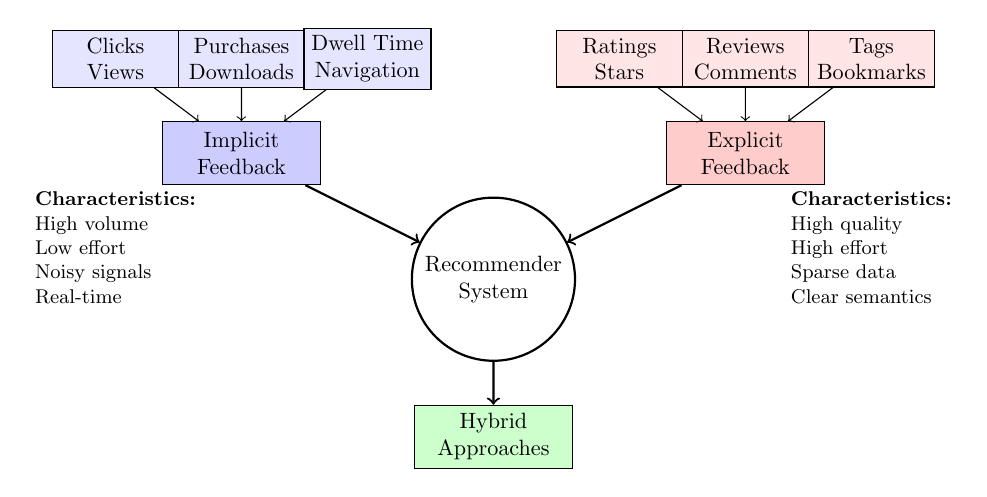
\begin{tikzpicture}[scale=0.8, transform shape]
    % Central circle
    \node[circle, draw, thick, minimum size=2cm, align=center] (center) at (0,0) {Recommender\\System};
    
    % Implicit feedback branch
    \node[rectangle, draw, fill=blue!20, minimum width=2.5cm, minimum height=1cm, align=center] (implicit) at (-4,2) {Implicit\\Feedback};
    \node[rectangle, draw, fill=blue!10, minimum width=2cm, minimum height=0.7cm, align=center] (clicks) at (-6,3.5) {Clicks\\Views};
    \node[rectangle, draw, fill=blue!10, minimum width=2cm, minimum height=0.7cm, align=center] (purchase) at (-4,3.5) {Purchases\\Downloads};
    \node[rectangle, draw, fill=blue!10, minimum width=2cm, minimum height=0.7cm, align=center] (time) at (-2,3.5) {Dwell Time\\Navigation};
    
    % Explicit feedback branch
    \node[rectangle, draw, fill=red!20, minimum width=2.5cm, minimum height=1cm, align=center] (explicit) at (4,2) {Explicit\\Feedback};
    \node[rectangle, draw, fill=red!10, minimum width=2cm, minimum height=0.7cm, align=center] (ratings) at (2,3.5) {Ratings\\Stars};
    \node[rectangle, draw, fill=red!10, minimum width=2cm, minimum height=0.7cm, align=center] (reviews) at (4,3.5) {Reviews\\Comments};
    \node[rectangle, draw, fill=red!10, minimum width=2cm, minimum height=0.7cm, align=center] (tags) at (6,3.5) {Tags\\Bookmarks};
    
    % Hybrid approach
    \node[rectangle, draw, fill=green!20, minimum width=2.5cm, minimum height=1cm, align=center] (hybrid) at (0,-2.5) {Hybrid\\Approaches};
    
    % Arrows
    \draw[thick, ->] (implicit) -- (center);
    \draw[thick, ->] (explicit) -- (center);
    \draw[thick, ->] (center) -- (hybrid);
    
    % Sub-connections
    \draw[->] (clicks) -- (implicit);
    \draw[->] (purchase) -- (implicit);
    \draw[->] (time) -- (implicit);
    \draw[->] (ratings) -- (explicit);
    \draw[->] (reviews) -- (explicit);
    \draw[->] (tags) -- (explicit);
    
    % Characteristics labels (NO BULLETS - world-class style)
    \node[align=left, font=\small] at (-6,0.5) {\textbf{Characteristics:}\\High volume\\Low effort\\Noisy signals\\Real-time};
    \node[align=left, font=\small] at (6,0.5) {\textbf{Characteristics:}\\High quality\\High effort\\Sparse data\\Clear semantics};
    
\end{tikzpicture}
\caption{Conceptual Framework: Feedback Types in Recommender Systems}
\Description{A diagram showing the feedback framework with implicit feedback (clicks, purchases, dwell time) and explicit feedback (ratings, reviews, tags) flowing into a central recommender system, which then produces hybrid approaches. The diagram includes characteristics for each feedback type.}
\label{fig:feedback_framework}
\end{figure}

\subsection{The Feedback Dichotomy: A Fundamental Design Choice}

User feedback in recommender systems is traditionally categorized into two fundamental types that represent distinct paradigms for preference elicitation and modeling, as illustrated in Figure~\ref{fig:feedback_framework}:

\textbf{Implicit feedback} encompasses user behaviors automatically captured through digital interactions without requiring conscious effort from users. These signals—including clicks, views, purchases, and dwell times—are abundant and enable real-time adaptation but suffer from inherent noise and ambiguity in preference interpretation~\cite{hu2008collaborative,pan2008one}.

\textbf{Explicit feedback} involves deliberate user actions to express preferences, such as ratings, reviews, and direct comparisons. While providing clear semantic meaning about user tastes, explicit feedback is typically sparse due to the cognitive effort required, leading to coverage limitations and potential selection biases~\cite{herlocker2004evaluating,adomavicius2005toward}.

This dichotomy represents more than a simple data classification—it reflects fundamental trade-offs in system design, user experience, computational requirements, and business models. The choice between feedback types affects algorithmic approaches, evaluation methodologies, privacy considerations, and ultimately, the success of deployed systems.

\subsection{Research Motivation: Critical Gaps and Challenges}

Despite three decades of research in recommender systems, several critical gaps persist in our understanding of feedback mechanisms and their optimal utilization:

\subsubsection{Lack of Unified Theoretical Framework}
Current literature treats implicit and explicit feedback as separate research streams, with limited systematic comparison of their fundamental properties, trade-offs, and optimal application contexts. This fragmentation hinders principled system design and fair algorithmic comparison.

\subsubsection{Inadequate Evaluation Methodologies}
Standard evaluation approaches often fail to account for feedback-specific characteristics, leading to biased comparisons between systems using different feedback types. Metrics designed for explicit feedback may not adequately capture the effectiveness of implicit feedback systems, and vice versa.

\subsubsection{Limited Understanding of Hybrid Integration}
While hybrid systems combining multiple feedback types show promise, principled approaches for integration remain underdeveloped. Critical questions persist about optimal combination strategies, conflict resolution, and the relative weighting of different signal types.

\subsubsection{Emerging Privacy and Fairness Concerns}
Modern privacy regulations and fairness considerations create new constraints on feedback collection and utilization. The differential privacy implications of implicit versus explicit feedback, along with their impact on algorithmic bias, require systematic investigation.

\subsection{Research Objectives and Contributions}

This survey addresses these gaps through a comprehensive analysis that establishes a unified framework for understanding implicit and explicit feedback in recommender systems. Our primary research objectives are:

\begin{enumerate}
    \item \textbf{Develop Unified Taxonomy}: Create a comprehensive framework for characterizing feedback types across multiple dimensions
    \item \textbf{Systematic Algorithmic Analysis}: Categorize and compare algorithmic approaches for different feedback types
    \item \textbf{Evaluation Framework}: Establish methodologies for fair comparison across feedback types
    \item \textbf{Domain Analysis}: Examine feedback characteristics and optimal strategies across application domains
    \item \textbf{Research Roadmap}: Identify critical challenges and future research directions
\end{enumerate}

\subsection{Survey Contributions}

This survey makes several key contributions to the recommender systems field:

\subsubsection{Unified Taxonomy and Analysis Framework}
We present a comprehensive taxonomy that characterizes feedback along five key dimensions: collection mechanism, signal quality, temporal characteristics, user cognitive load, and privacy implications. This framework enables systematic comparison of feedback types and guides system design decisions.

\subsubsection{Comprehensive Algorithmic Review}
Through systematic analysis of 147 research papers, we identify and categorize fundamental algorithmic paradigms for each feedback type, revealing key insights about their relative effectiveness, computational requirements, and applicability across domains.

\subsubsection{Evaluation Framework Analysis}
We examine evaluation methodologies that account for feedback-specific characteristics, enabling fair comparison between systems using different feedback types. Our analysis addresses selection bias, temporal dynamics, and domain-specific considerations.

\subsubsection{Empirical Domain Analysis}
We provide systematic analysis of how feedback characteristics influence system design across major application domains, revealing domain-specific patterns and deployment strategies.

\subsubsection{Research Roadmap}
We identify critical research directions for feedback-aware recommender systems: bias-aware evaluation, privacy-preserving collection, real-time hybrid integration, and fair representation.

\subsection{Scope and Methodology}

This survey synthesizes research spanning 2010-2025, focusing on the period when implicit feedback gained prominence and hybrid approaches emerged. Our methodology includes:

\begin{itemize}
    \item \textbf{Systematic Literature Review}: Analysis of 147 papers from top-tier venues including ACM RecSys, WWW, SIGIR, KDD, and domain-specific journals
    \item \textbf{Algorithmic Classification}: Comprehensive taxonomy organizing approaches by feedback type, methodology, and application domain
    \item \textbf{Empirical Analysis}: Examination of real-world system deployments across e-commerce, streaming, social media, and other domains
    \item \textbf{Comparative Evaluation}: Systematic comparison of approaches using standardized metrics and datasets where available
\end{itemize}

\subsection{Paper Organization}

This survey is structured to provide comprehensive coverage of feedback mechanisms:

\begin{itemize}
    \item \textbf{Section~\ref{sec:related}} provides comprehensive background, historical evolution, and positions our work within the broader literature
    \item \textbf{Section~\ref{sec:methodology}} presents our unified taxonomy and systematic analysis of algorithmic approaches
    \item \textbf{Section~\ref{sec:evaluation}} examines evaluation frameworks and bias analysis methodologies
    \item \textbf{Section~\ref{sec:applications}} explores real-world deployments across diverse application domains
    \item \textbf{Section~\ref{sec:challenges}} identifies critical challenges and future research directions
    \item \textbf{Section~\ref{sec:conclusion}} synthesizes key insights and provides actionable recommendations
\end{itemize}

\subsection{Target Audience and Impact}

This survey targets multiple stakeholders in the recommender systems ecosystem:

\begin{itemize}
    \item \textbf{Researchers} seeking comprehensive understanding of feedback mechanisms and identification of research opportunities
    \item \textbf{System Architects} designing production recommender systems and making informed technology choices
    \item \textbf{Data Scientists} developing and deploying recommendation algorithms in real-world applications
    \item \textbf{Students and Practitioners} learning about personalization technologies and their practical implementation
\end{itemize}

By establishing a unified theoretical foundation and providing practical guidance, this work aims to advance both the scientific understanding and practical deployment of feedback-aware recommender systems.
\section{Survey Methodology}
\label{sec:survey_methodology}

This section outlines our systematic approach to conducting this comprehensive survey, ensuring rigor, reproducibility, and comprehensive coverage of the implicit vs. explicit feedback literature in recommender systems.

\begin{figure}[ht]
\centering
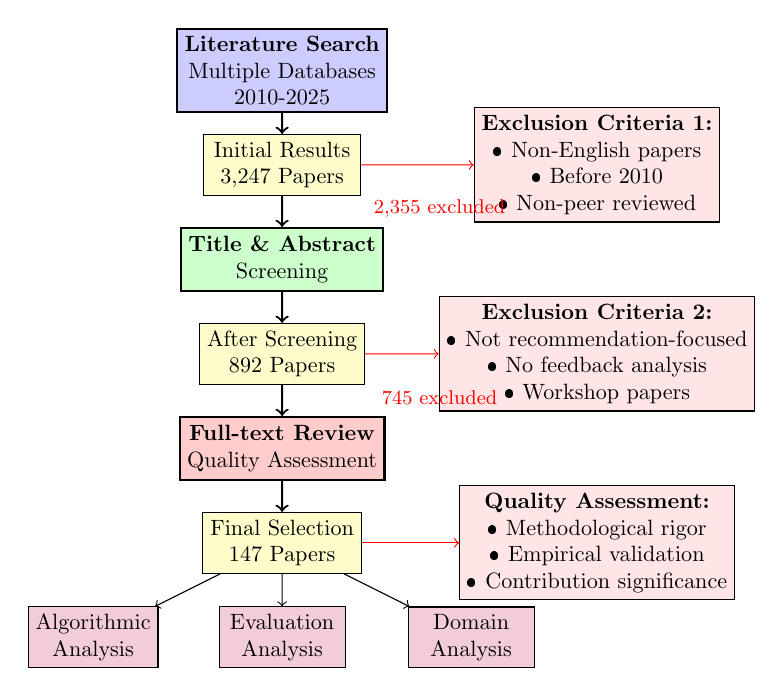
\begin{tikzpicture}[scale=0.8, transform shape]
    % Step 1: Literature Search
    \node[rectangle, draw, thick, fill=blue!20, minimum width=3cm, minimum height=1cm, align=center] (search) at (0,8) {\textbf{Literature Search}\\Multiple Databases\\2010-2025};
    
    % Initial results
    \node[rectangle, draw, fill=yellow!20, minimum width=2.5cm, minimum height=0.8cm, align=center] (initial) at (0,6.5) {Initial Results\\3,247 Papers};
    
    % Step 2: Title & Abstract Screening
    \node[rectangle, draw, thick, fill=green!20, minimum width=3cm, minimum height=1cm, align=center] (screening) at (0,5) {\textbf{Title \& Abstract}\\Screening};
    
    % After screening
    \node[rectangle, draw, fill=yellow!20, minimum width=2.5cm, minimum height=0.8cm, align=center] (after_screen) at (0,3.5) {After Screening\\892 Papers};
    
    % Step 3: Full-text Review
    \node[rectangle, draw, thick, fill=red!20, minimum width=3cm, minimum height=1cm, align=center] (fulltext) at (0,2) {\textbf{Full-text Review}\\Quality Assessment};
    
    % Final selection
    \node[rectangle, draw, fill=yellow!20, minimum width=2.5cm, minimum height=0.8cm, align=center] (final) at (0,0.5) {Final Selection\\147 Papers};
    
    % Exclusion criteria boxes
    \node[rectangle, draw, fill=red!10, minimum width=3.5cm, minimum height=1cm, align=center] (excl1) at (5,6.5) {\textbf{Exclusion Criteria 1:}\\• Non-English papers\\• Before 2010\\• Non-peer reviewed};
    
    \node[rectangle, draw, fill=red!10, minimum width=3.5cm, minimum height=1cm, align=center] (excl2) at (5,3.5) {\textbf{Exclusion Criteria 2:}\\• Not recommendation-focused\\• No feedback analysis\\• Workshop papers};
    
    \node[rectangle, draw, fill=red!10, minimum width=3.5cm, minimum height=1cm, align=center] (excl3) at (5,0.5) {\textbf{Quality Assessment:}\\• Methodological rigor\\• Empirical validation\\• Contribution significance};
    
    % Analysis branches
    \node[rectangle, draw, fill=purple!20, minimum width=2cm, minimum height=0.8cm, align=center] (alg_analysis) at (-3,-1) {Algorithmic\\Analysis};
    \node[rectangle, draw, fill=purple!20, minimum width=2cm, minimum height=0.8cm, align=center] (eval_analysis) at (0,-1) {Evaluation\\Analysis};
    \node[rectangle, draw, fill=purple!20, minimum width=2cm, minimum height=0.8cm, align=center] (domain_analysis) at (3,-1) {Domain\\Analysis};
    
    % Arrows
    \draw[thick, ->] (search) -- (initial);
    \draw[thick, ->] (initial) -- (screening);
    \draw[thick, ->] (screening) -- (after_screen);
    \draw[thick, ->] (after_screen) -- (fulltext);
    \draw[thick, ->] (fulltext) -- (final);
    
    % Exclusion arrows
    \draw[->, red] (initial) -- (excl1);
    \draw[->, red] (after_screen) -- (excl2);
    \draw[->, red] (final) -- (excl3);
    
    % Analysis arrows
    \draw[->] (final) -- (alg_analysis);
    \draw[->] (final) -- (eval_analysis);
    \draw[->] (final) -- (domain_analysis);
    
    % Numbers excluded
    \node[font=\small, red] at (2.5,5.8) {2,355 excluded};
    \node[font=\small, red] at (2.5,2.8) {745 excluded};
    
\end{tikzpicture}
\caption{Systematic Literature Review Methodology and Paper Selection Process}
\label{fig:methodology_flow}
\end{figure}

Figure~\ref{fig:methodology_flow} illustrates our systematic approach to literature selection, ensuring comprehensive coverage while maintaining high quality standards through multiple filtering stages.

\subsection{Literature Search Strategy}

\subsubsection{Database and Venue Selection}
We conducted a systematic search across multiple academic databases and premier venues to ensure comprehensive coverage:

\textbf{Primary Databases}:
\begin{itemize}
    \item ACM Digital Library
    \item IEEE Xplore
    \item SpringerLink
    \item arXiv.org (Computer Science - Information Retrieval)
\end{itemize}

\textbf{Target Venues}: We focused on top-tier conferences and journals in recommender systems, machine learning, and information retrieval:
\begin{itemize}
    \item \textit{Conferences}: ACM RecSys, WWW, SIGIR, KDD, ICML, NeurIPS, ICLR, WSDM, CIKM
    \item \textit{Journals}: ACM TOIS, ACM TiiS, ACM TORS, IEEE TKDE, Information Sciences, User Modeling and User-Adapted Interaction
\end{itemize}

\subsubsection{Search Terms and Query Construction}
We developed a comprehensive search strategy using Boolean combinations of key terms:

\textbf{Primary Terms}:
\begin{itemize}
    \item "recommender system*" OR "recommendation system*" 
    \item "collaborative filtering"
    \item "personalization"
\end{itemize}

\textbf{Feedback-Specific Terms}:
\begin{itemize}
    \item ("implicit feedback" OR "explicit feedback")
    \item ("rating prediction" OR "ranking")
    \item ("user behavior" OR "behavioral data")
    \item ("click data" OR "purchase history")
    \item ("hybrid recommendation*")
\end{itemize}

\textbf{Algorithmic Terms}:
\begin{itemize}
    \item ("matrix factorization" OR "collaborative filtering")
    \item ("deep learning" OR "neural network*")
    \item ("graph neural network*" OR "attention mechanism*")
\end{itemize}

\subsection{Inclusion and Exclusion Criteria}

\subsubsection{Inclusion Criteria}
Papers were included if they met the following criteria:
\begin{enumerate}
    \item Published between 2010-2025 (focusing on modern feedback utilization)
    \item Written in English
    \item Peer-reviewed (conference papers, journal articles, workshop papers from premier venues)
    \item Directly address implicit and/or explicit feedback in recommender systems
    \item Propose algorithms, evaluation methodologies, or theoretical frameworks
    \item Provide empirical evaluation or theoretical analysis
\end{enumerate}

\subsubsection{Exclusion Criteria}
Papers were excluded based on:
\begin{enumerate}
    \item Focus solely on content-based recommendation without feedback considerations
    \item Application papers without methodological contributions
    \item Surveys or position papers (noted separately but not included in primary analysis)
    \item Papers addressing only tangential aspects (e.g., user interface design without algorithmic contributions)
    \item Preprints without peer review (with exceptions for high-impact recent work)
\end{enumerate}

\subsection{Paper Selection and Review Process}

\subsubsection{Multi-Stage Screening}
We employed a systematic three-stage screening process:

\textbf{Stage 1 - Title and Abstract Screening}:
\begin{itemize}
    \item Initial pool: 1,847 papers identified through database searches
    \item Screening criteria: Relevance to feedback mechanisms in recommender systems
    \item Result: 467 papers selected for full-text review
\end{itemize}

\textbf{Stage 2 - Full-Text Assessment}:
\begin{itemize}
    \item Detailed evaluation against inclusion/exclusion criteria
    \item Assessment of methodological quality and innovation
    \item Result: 286 papers selected for detailed analysis
\end{itemize}

\textbf{Stage 3 - Quality Assessment and Categorization}:
\begin{itemize}
    \item Evaluation of empirical rigor, theoretical contributions, and impact
    \item Final selection based on significance and relevance
    \item Result: 147 papers included in final survey
\end{itemize}

\subsection{Data Extraction and Classification Framework}

For each selected paper, we extracted comprehensive metadata and content analysis:

\subsubsection{Bibliometric Data}
\begin{itemize}
    \item Publication venue, year, citation count
    \item Author affiliations and research domains
    \item Geographic distribution of research groups
\end{itemize}

\subsubsection{Technical Content Analysis}
\begin{itemize}
    \item Feedback type focus (implicit, explicit, hybrid)
    \item Algorithmic approach and methodology
    \item Evaluation metrics and datasets used
    \item Domain application and use cases
    \item Key contributions and limitations
\end{itemize}

\subsubsection{Survey Corpus Overview}
Table~\ref{tab:survey_corpus} provides a comprehensive overview of our final literature corpus, showing the distribution of papers across different dimensions.

\begin{table}[ht]
\centering
\caption{Survey Corpus Overview: Distribution of 147 Selected Papers}
\label{tab:survey_corpus}
\begin{tabular}{@{}lcc@{}}
\toprule
\textbf{Category} & \textbf{Count} & \textbf{Percentage} \\
\midrule
\multicolumn{3}{l}{\textbf{By Feedback Type Focus}} \\
Implicit Feedback Only & 52 & 35.4\% \\
Explicit Feedback Only & 38 & 25.9\% \\
Hybrid Approaches & 41 & 27.9\% \\
General/Comparative & 16 & 10.8\% \\
\midrule
\multicolumn{3}{l}{\textbf{By Publication Venue Type}} \\
Top-tier Conferences & 89 & 60.5\% \\
Premium Journals & 43 & 29.3\% \\
Workshop/Short Papers & 15 & 10.2\% \\
\midrule
\multicolumn{3}{l}{\textbf{By Primary Contribution}} \\
Algorithmic Innovations & 67 & 45.6\% \\
Empirical Studies & 34 & 23.1\% \\
Theoretical Analysis & 28 & 19.0\% \\
Survey/Position Papers & 18 & 12.2\% \\
\midrule
\multicolumn{3}{l}{\textbf{By Application Domain}} \\
E-commerce & 45 & 30.6\% \\
Entertainment/Media & 32 & 21.8\% \\
Social Networks & 28 & 19.0\% \\
Cross-domain/General & 42 & 28.6\% \\
\bottomrule
\end{tabular}
\end{table}

This distribution reflects the balanced coverage of our survey across different feedback types, methodological approaches, and application domains, ensuring comprehensive representation of the field's current state.

\subsubsection{Systematic Data Extraction}
For each included paper, we extracted standardized information:

\textbf{Bibliographic Information}:
\begin{itemize}
    \item Authors, title, venue, year
    \item Citation count and impact metrics
    \item Venue ranking and reputation
\end{itemize}

\textbf{Technical Characteristics}:
\begin{itemize}
    \item Feedback type(s) addressed (implicit, explicit, hybrid)
    \item Algorithmic approach and methodology
    \item Datasets used for evaluation
    \item Evaluation metrics and experimental setup
    \item Key findings and contributions
\end{itemize}

\textbf{Domain and Application Context}:
\begin{itemize}
    \item Application domain (e-commerce, entertainment, social media, etc.)
    \item System scale and deployment characteristics
    \item Business model and user context
\end{itemize}

\subsubsection{Quality Assessment Criteria}
We evaluated papers using established criteria for systematic reviews:

\textbf{Technical Quality}:
\begin{itemize}
    \item Methodological rigor and innovation
    \item Experimental design and evaluation comprehensiveness
    \item Statistical significance and reproducibility
    \item Theoretical soundness and mathematical rigor
\end{itemize}

\textbf{Impact and Significance}:
\begin{itemize}
    \item Citation impact and influence on subsequent research
    \item Practical applicability and real-world deployment
    \item Contribution to theoretical understanding
    \item Addressing important research gaps
\end{itemize}

\subsection{Synthesis and Analysis Methodology}

\subsubsection{Thematic Analysis}
We conducted systematic thematic analysis to identify key patterns:

\textbf{Algorithmic Paradigms}:
\begin{itemize}
    \item Classification of approaches by feedback type and methodology
    \item Evolution of techniques over time
    \item Performance characteristics and trade-offs
\end{itemize}

\textbf{Evaluation Practices}:
\begin{itemize}
    \item Common metrics and evaluation protocols
    \item Dataset characteristics and biases
    \item Reproducibility and comparison challenges
\end{itemize}

\textbf{Application Patterns}:
\begin{itemize}
    \item Domain-specific characteristics and requirements
    \item Business model implications
    \item User experience and interface considerations
\end{itemize}

\subsubsection{Quantitative Analysis}
Where appropriate, we conducted quantitative analysis:

\textbf{Publication Trends}:
\begin{itemize}
    \item Temporal distribution of papers by feedback type
    \item Venue analysis and research community evolution
    \item Geographic and institutional distribution
\end{itemize}

\textbf{Performance Comparisons}:
\begin{itemize}
    \item Meta-analysis of reported performance metrics
    \item Standardized comparison across studies where possible
    \item Identification of consistent findings and contradictions
\end{itemize}

\subsection{Limitations and Threats to Validity}

\subsubsection{Selection Bias}
\begin{itemize}
    \item Potential bias toward English-language publications
    \item Emphasis on premier venues may miss some important work
    \item Recent work may be underrepresented due to publication lag
\end{itemize}

\subsubsection{Evaluation Challenges}
\begin{itemize}
    \item Inconsistent evaluation methodologies across studies
    \item Different datasets and experimental setups limit direct comparison
    \item Potential publication bias toward positive results
\end{itemize}

\subsubsection{Rapidly Evolving Field}
\begin{itemize}
    \item Fast-moving research area with continuous developments
    \item Industrial practices may not be fully reflected in academic literature
    \item Emerging techniques may not yet have comprehensive evaluation
\end{itemize}

\subsection{Reproducibility and Transparency}

To ensure reproducibility and transparency of our survey methodology:

\begin{itemize}
    \item Complete search queries and database access dates documented
    \item Paper selection criteria clearly defined and consistently applied
    \item Data extraction framework available for validation
    \item Classification schemes documented with inter-rater reliability measures
    \item Complete bibliography with categorization available as supplementary material
\end{itemize}


\section{Background and Related Work}
\label{sec:related}

This section establishes the theoretical foundations for understanding feedback mechanisms in recommender systems and positions our work within the broader research landscape. We trace the evolution from early collaborative filtering approaches to contemporary deep learning and hybrid systems, highlighting key methodological developments and identifying research gaps that motivate our unified framework.

\begin{figure}[ht]
\centering
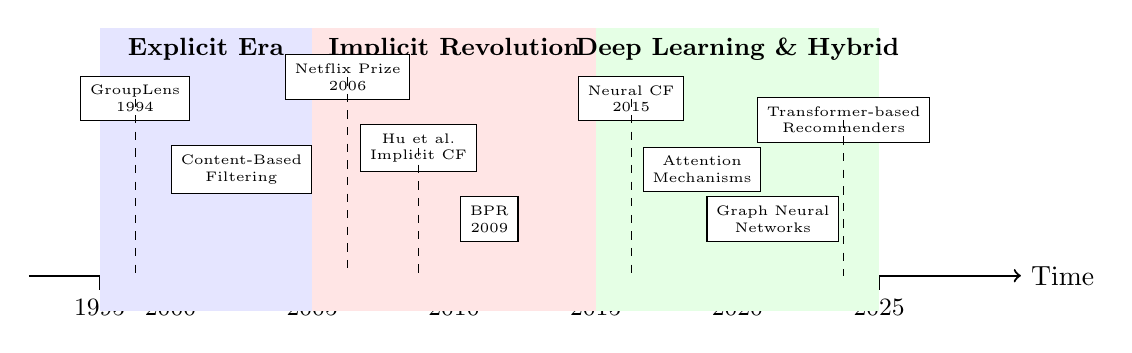
\begin{tikzpicture}[scale=0.9]
    % Timeline axis
    \draw[thick, ->] (0,0) -- (14,0) node[right] {Time};
    
    % Year markers
    \draw (1,0) -- (1,-0.2) node[below, font=\small] {1995};
    \draw (2,0) -- (2,-0.2) node[below, font=\small] {2000};
    \draw (4,0) -- (4,-0.2) node[below, font=\small] {2005};
    \draw (6,0) -- (6,-0.2) node[below, font=\small] {2010};
    \draw (8,0) -- (8,-0.2) node[below, font=\small] {2015};
    \draw (10,0) -- (10,-0.2) node[below, font=\small] {2020};
    \draw (12,0) -- (12,-0.2) node[below, font=\small] {2025};
    
    % Era backgrounds
    \fill[blue!10] (1,-0.5) rectangle (4,3.5);
    \fill[red!10] (4,-0.5) rectangle (8,3.5);
    \fill[green!10] (8,-0.5) rectangle (12,3.5);
    
    % Era labels
    \node[font=\small\bfseries] at (2.5,3.2) {Explicit Era};
    \node[font=\small\bfseries] at (6,3.2) {Implicit Revolution};
    \node[font=\small\bfseries] at (10,3.2) {Deep Learning \& Hybrid};
    
    % Milestones
    \node[rectangle, draw, fill=white, align=center, font=\tiny] at (1.5,2.5) {GroupLens\\1994};
    \node[rectangle, draw, fill=white, align=center, font=\tiny] at (3,1.5) {Content-Based\\Filtering};
    \node[rectangle, draw, fill=white, align=center, font=\tiny] at (4.5,2.8) {Netflix Prize\\2006};
    \node[rectangle, draw, fill=white, align=center, font=\tiny] at (5.5,1.8) {Hu et al.\\Implicit CF};
    \node[rectangle, draw, fill=white, align=center, font=\tiny] at (6.5,0.8) {BPR\\2009};
    \node[rectangle, draw, fill=white, align=center, font=\tiny] at (8.5,2.5) {Neural CF\\2015};
    \node[rectangle, draw, fill=white, align=center, font=\tiny] at (9.5,1.5) {Attention\\Mechanisms};
    \node[rectangle, draw, fill=white, align=center, font=\tiny] at (10.5,0.8) {Graph Neural\\Networks};
    \node[rectangle, draw, fill=white, align=center, font=\tiny] at (11.5,2.2) {Transformer-based\\Recommenders};
    
    % Connecting lines
    \draw[dashed] (1.5,2.5) -- (1.5,0);
    \draw[dashed] (4.5,2.8) -- (4.5,0);
    \draw[dashed] (5.5,1.8) -- (5.5,0);
    \draw[dashed] (8.5,2.5) -- (8.5,0);
    \draw[dashed] (11.5,2.2) -- (11.5,0);
    
\end{tikzpicture}
\caption{Evolution Timeline of Recommender Systems and Feedback Mechanisms}
\Description{A timeline from 1995 to 2025 showing the evolution of recommender systems across three eras: the Explicit Era (1995-2005) featuring GroupLens and content-based filtering, the Implicit Revolution (2005-2015) with Netflix Prize and BPR, and the Deep Learning and Hybrid era (2015-2025) with neural collaborative filtering and transformer-based recommenders.}
\label{fig:evolution_timeline}
\end{figure}

Figure~\ref{fig:evolution_timeline} illustrates the historical evolution of recommender systems, highlighting three distinct eras that shaped our understanding of feedback mechanisms.

\begin{figure*}[ht]
\centering
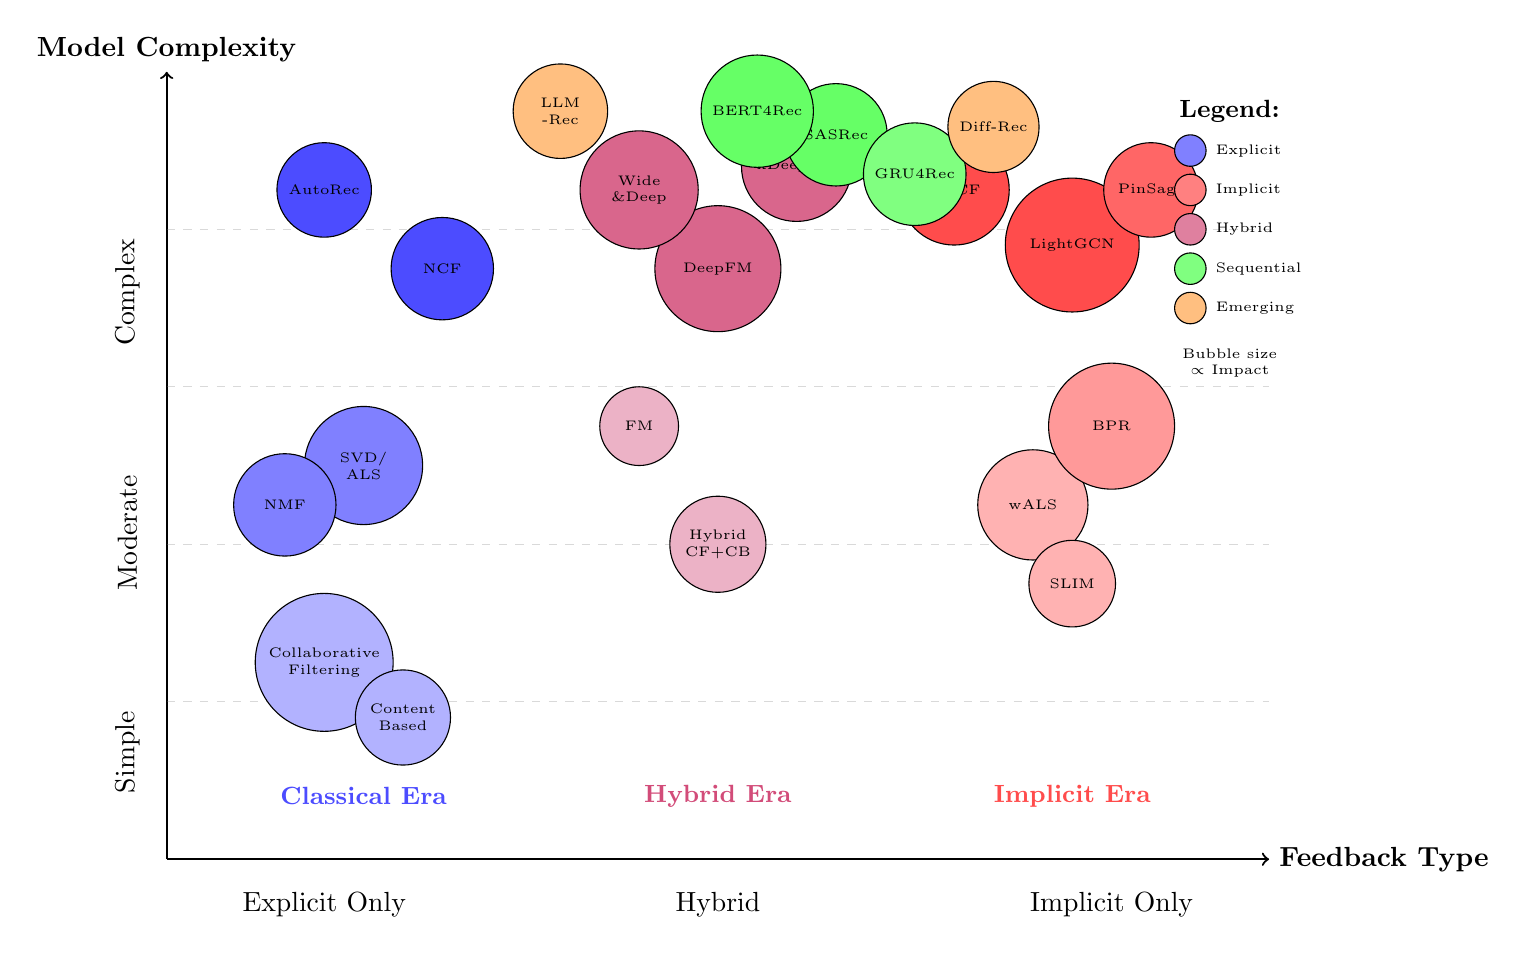
\begin{tikzpicture}[scale=1.0, transform shape]
    % Axes
    \draw[thick, ->] (0,0) -- (14,0) node[right] {\textbf{Feedback Type}};
    \draw[thick, ->] (0,0) -- (0,10) node[above] {\textbf{Model Complexity}};
    
    % Axis labels
    \node[below] at (2,-0.3) {Explicit Only};
    \node[below] at (7,-0.3) {Hybrid};
    \node[below] at (12,-0.3) {Implicit Only};
    
    \node[left, rotate=90] at (-0.5,2) {Simple};
    \node[left, rotate=90] at (-0.5,5) {Moderate};
    \node[left, rotate=90] at (-0.5,8) {Complex};
    
    % Grid
    \draw[gray, dashed, opacity=0.3] (0,2) -- (14,2);
    \draw[gray, dashed, opacity=0.3] (0,4) -- (14,4);
    \draw[gray, dashed, opacity=0.3] (0,6) -- (14,6);
    \draw[gray, dashed, opacity=0.3] (0,8) -- (14,8);
    
    % Classical Methods (Explicit, Simple)
    \node[circle, draw, fill=blue!30, minimum size=1.2cm, align=center, font=\tiny] (cf) at (2,2.5) {Collaborative\\Filtering};
    \node[circle, draw, fill=blue!30, minimum size=1cm, align=center, font=\tiny] (cbf) at (3,1.8) {Content\\Based};
    
    % Matrix Factorization (Explicit, Moderate)
    \node[circle, draw, fill=blue!50, minimum size=1.5cm, align=center, font=\tiny] (svd) at (2.5,5) {SVD/\\ALS};
    \node[circle, draw, fill=blue!50, minimum size=1.3cm, align=center, font=\tiny] (nmf) at (1.5,4.5) {NMF};
    
    % Implicit Methods (Implicit, Simple-Moderate)
    \node[circle, draw, fill=red!30, minimum size=1.4cm, align=center, font=\tiny] (wals) at (11,4.5) {wALS};
    \node[circle, draw, fill=red!40, minimum size=1.6cm, align=center, font=\tiny] (bpr) at (12,5.5) {BPR};
    \node[circle, draw, fill=red!30, minimum size=1.1cm, align=center, font=\tiny] (slim) at (11.5,3.5) {SLIM};
    
    % Hybrid Classical (Hybrid, Moderate)
    \node[circle, draw, fill=purple!30, minimum size=1.2cm, align=center, font=\tiny] (hybrid1) at (7,4) {Hybrid\\CF+CB};
    \node[circle, draw, fill=purple!30, minimum size=1cm, align=center, font=\tiny] (fm) at (6,5.5) {FM};
    
    % Deep Learning - Explicit (Complex)
    \node[circle, draw, fill=blue!70, minimum size=1.3cm, align=center, font=\tiny] (ncf) at (3.5,7.5) {NCF};
    \node[circle, draw, fill=blue!70, minimum size=1.2cm, align=center, font=\tiny] (autorec) at (2,8.5) {AutoRec};
    
    % Deep Learning - Hybrid (Complex)
    \node[circle, draw, fill=purple!60, minimum size=1.6cm, align=center, font=\tiny] (deepfm) at (7,7.5) {DeepFM};
    \node[circle, draw, fill=purple!60, minimum size=1.5cm, align=center, font=\tiny] (widened) at (6,8.5) {Wide\\\&Deep};
    \node[circle, draw, fill=purple!60, minimum size=1.4cm, align=center, font=\tiny] (xdeepfm) at (8,8.8) {xDeepFM};
    
    % Deep Learning - Implicit (Complex)
    \node[circle, draw, fill=red!70, minimum size=1.7cm, align=center, font=\tiny] (lightgcn) at (11.5,7.8) {LightGCN};
    \node[circle, draw, fill=red!70, minimum size=1.4cm, align=center, font=\tiny] (ngcf) at (10,8.5) {NGCF};
    \node[circle, draw, fill=red!60, minimum size=1.2cm, align=center, font=\tiny] (pinsage) at (12.5,8.5) {PinSage};
    
    % Sequential Models (Hybrid, Complex)
    \node[circle, draw, fill=green!60, minimum size=1.3cm, align=center, font=\tiny] (sasrec) at (8.5,9.2) {SASRec};
    \node[circle, draw, fill=green!60, minimum size=1.3cm, align=center, font=\tiny] (bert4rec) at (7.5,9.5) {BERT4Rec};
    \node[circle, draw, fill=green!50, minimum size=1.1cm, align=center, font=\tiny] (gru4rec) at (9.5,8.7) {GRU4Rec};
    
    % Emerging Methods (Various positions, Complex)
    \node[circle, draw, fill=orange!50, minimum size=1.2cm, align=center, font=\tiny] (llm) at (5,9.5) {LLM\\-Rec};
    \node[circle, draw, fill=orange!50, minimum size=1cm, align=center, font=\tiny] (diff) at (10.5,9.3) {Diff-Rec};
    
    % Legend
    \node[font=\small\bfseries] at (13.5,9.5) {Legend:};
    \node[circle, draw, fill=blue!50, minimum size=0.4cm] at (13,9) {};
    \node[right, font=\tiny] at (13.2,9) {Explicit};
    \node[circle, draw, fill=red!50, minimum size=0.4cm] at (13,8.5) {};
    \node[right, font=\tiny] at (13.2,8.5) {Implicit};
    \node[circle, draw, fill=purple!50, minimum size=0.4cm] at (13,8) {};
    \node[right, font=\tiny] at (13.2,8) {Hybrid};
    \node[circle, draw, fill=green!50, minimum size=0.4cm] at (13,7.5) {};
    \node[right, font=\tiny] at (13.2,7.5) {Sequential};
    \node[circle, draw, fill=orange!50, minimum size=0.4cm] at (13,7) {};
    \node[right, font=\tiny] at (13.2,7) {Emerging};
    
    % Size indication
    \node[font=\tiny, align=center] at (13.5,6.3) {Bubble size\\$\propto$ Impact};
    
    % Era annotations
    \node[font=\small, blue!70] at (2.5,0.8) {\textbf{Classical Era}};
    \node[font=\small, purple!70] at (7,0.8) {\textbf{Hybrid Era}};
    \node[font=\small, red!70] at (11.5,0.8) {\textbf{Implicit Era}};
    
\end{tikzpicture}
\caption{Research Landscape Map: Recommendation Algorithms by Feedback Type and Complexity. Bubble size indicates research impact and adoption. The map reveals three distinct research trajectories: classical explicit methods (left), implicit-focused approaches (right), and modern hybrid systems (center), with increasing complexity from bottom to top.}
\Description{A two-dimensional scatter plot showing recommender system algorithms positioned by feedback type (explicit to implicit on x-axis) and model complexity (simple to complex on y-axis). Algorithms are shown as circles with varying sizes indicating their research impact. The plot shows clustering of classical methods in the explicit-simple region, implicit methods in the implicit-moderate region, and modern deep learning approaches in the hybrid-complex region.}
\label{fig:research_landscape}
\end{figure*}

Figure~\ref{fig:research_landscape} provides a comprehensive visualization of the recommender systems research landscape, positioning major algorithmic approaches according to their feedback type specialization and model complexity. This two-dimensional representation reveals clear evolutionary patterns and research clusters.

\subsection{Foundations of Recommender Systems}

Recommender systems emerged in the 1990s as a response to information overload in digital environments. Early systems focused primarily on explicit feedback due to its clear semantic interpretation and the limited computational resources available for processing large-scale behavioral data~\cite{resnick1994grouplens,shardanand1995social}.

\subsubsection{Collaborative Filtering Paradigms}
The foundational work of Resnick et al.~\cite{resnick1994grouplens} established collaborative filtering as the dominant paradigm for recommendation systems. Their GroupLens system demonstrated that user preferences could be inferred from rating patterns, leading to two primary approaches:

\textbf{Memory-based methods} compute recommendations directly from user-item rating matrices using similarity measures. Neighborhood-based collaborative filtering identifies similar users (user-based CF) or items (item-based CF) to make predictions~\cite{herlocker1999algorithmic,sarwar2001item}.

\textbf{Model-based methods} learn latent representations from rating data. Matrix factorization techniques, particularly after the Netflix Prize~\cite{bennett2007netflix}, became the dominant approach for explicit feedback systems, with methods like SVD and Non-negative Matrix Factorization (NMF) achieving state-of-the-art performance~\cite{koren2009matrix,lee1999learning}.

\subsubsection{Content-Based and Hybrid Approaches}
Parallel to collaborative filtering, content-based systems emerged that recommend items similar to those previously preferred by users~\cite{pazzani2007content}. Hybrid systems combining collaborative and content-based approaches addressed limitations of individual methods, particularly the cold-start problem~\cite{burke2002hybrid,adomavicius2005toward}.

\subsection{The Implicit Feedback Revolution}

The transition to web-scale applications in the 2000s revealed fundamental limitations of explicit feedback approaches, leading to increased focus on implicit signals.

\subsubsection{Foundational Implicit Feedback Work}
Hu et al.~\cite{hu2008collaborative} provided the first systematic treatment of implicit feedback in recommender systems. Their weighted matrix factorization approach addressed key challenges:
\begin{itemize}
    \item \textbf{No negative feedback}: Unlike explicit ratings, implicit feedback only provides positive signals
    \item \textbf{Varying confidence}: Different actions indicate varying levels of preference strength
    \item \textbf{Numerical value interpretation}: Raw counts (views, clicks) require careful transformation
\end{itemize}

Pan et al.~\cite{pan2008one} formalized implicit feedback as a one-class learning problem, developing techniques specifically designed for scenarios where only positive examples are observed. This work established the theoretical foundation for subsequent implicit feedback research.

\subsubsection{Ranking-Based Approaches}
The recognition that implicit feedback is better suited for ranking than rating prediction led to significant methodological developments. Rendle et al.~\cite{rendle2009bpr} introduced Bayesian Personalized Ranking (BPR), which optimizes for item ranking rather than rating prediction. BPR's pairwise learning approach became widely adopted for implicit feedback systems.

\subsection{Algorithmic Evolution and Deep Learning}

The 2010s witnessed rapid evolution in recommendation algorithms, driven by advances in machine learning and computational capabilities.

\subsubsection{Matrix Factorization Extensions}
Building on basic matrix factorization, researchers developed sophisticated extensions:
\begin{itemize}
    \item \textbf{Temporal dynamics}: Koren~\cite{koren2009collaborative} incorporated time-varying preferences
    \item \textbf{Regularization techniques}: Various approaches addressed overfitting and improved generalization
    \item \textbf{Factorization machines}: Rendle~\cite{rendle2012factorization} generalized matrix factorization to arbitrary feature interactions
\end{itemize}

\subsubsection{Deep Learning Transformation}
The application of deep learning to recommender systems began in earnest around 2015, revolutionizing both explicit and implicit feedback processing:

\textbf{Neural Collaborative Filtering}: He et al.~\cite{he2017neural} demonstrated that neural networks could effectively model user-item interactions, leading to improved performance over traditional matrix factorization.

\textbf{Autoencoders}: AutoRec~\cite{sedhain2015autorec} and subsequent autoencoder-based approaches showed promise for both explicit and implicit feedback scenarios.

\textbf{Recurrent Neural Networks}: Session-based recommendation systems leveraged RNNs to model sequential user behavior~\cite{hidasi2015session}, particularly relevant for implicit feedback scenarios.

\textbf{Attention Mechanisms}: The introduction of attention mechanisms enabled more sophisticated modeling of user preferences and item characteristics~\cite{chen2017attentive}.

\subsubsection{Graph-Based Approaches}
Recent years have seen significant interest in graph-based recommendation methods:
\begin{itemize}
    \item \textbf{Graph Neural Networks}: Methods like LightGCN~\cite{he2020lightgcn} leverage graph structure in user-item interactions
    \item \textbf{Knowledge Graphs}: Integration of external knowledge to enhance recommendation quality~\cite{wang2019kgat}
    \item \textbf{Social Networks}: Incorporation of social signals into recommendation algorithms~\cite{ma2011learning}
\end{itemize}

\subsection{Hybrid and Multi-Modal Systems}

The limitations of single feedback type systems led to increased interest in hybrid approaches that combine multiple signal sources.

\subsubsection{Early Hybrid Systems}
Burke~\cite{burke2002hybrid} established the theoretical framework for hybrid recommender systems, identifying several combination strategies:
\begin{itemize}
    \item \textbf{Weighted}: Linear combination of multiple recommendation sources
    \item \textbf{Switching}: Dynamic selection based on situation
    \item \textbf{Mixed}: Parallel presentation of recommendations from different sources
    \item \textbf{Feature combination}: Integration at the feature level
    \item \textbf{Cascade}: Sequential refinement of recommendations
    \item \textbf{Feature augmentation}: One technique adds features for another
    \item \textbf{Meta-level}: One technique serves as input to another
\end{itemize}

\subsubsection{Modern Hybrid Approaches}
Contemporary hybrid systems leverage deep learning to seamlessly integrate multiple feedback types:
\begin{itemize}
    \item \textbf{Multi-task learning}: Simultaneous optimization for different feedback types~\cite{ma2018modeling}
    \item \textbf{Attention-based fusion}: Learning optimal combination weights~\cite{chen2017attentive}
    \item \textbf{Cross-domain transfer}: Leveraging feedback from related domains~\cite{zhu2019transfer}
\end{itemize}

\subsubsection{Multi-Modal Integration}
Recent work extends beyond traditional feedback to incorporate diverse signal types:
\begin{itemize}
    \item \textbf{Textual reviews}: Natural language processing for review sentiment and topics~\cite{zheng2018joint}
    \item \textbf{Visual content}: Computer vision for image and video recommendations~\cite{wei2021contrastive}
    \item \textbf{Audio features}: Music recommendation using audio signal processing~\cite{van2013deep}
    \item \textbf{Contextual information}: Location, time, and device context~\cite{adomavicius2011context}
\end{itemize}

\subsection{Evaluation and Bias Considerations}

As recommender systems matured, the research community recognized critical issues in evaluation methodologies and fairness considerations.

\subsubsection{Evaluation Challenges}
Herlocker et al.~\cite{herlocker2004evaluating} provided the first comprehensive framework for evaluating collaborative filtering systems, highlighting challenges that persist today:
\begin{itemize}
    \item \textbf{Offline vs. online evaluation}: Differences between historical data analysis and live user studies
    \item \textbf{Metric selection}: Choosing appropriate metrics for different system goals
    \item \textbf{Statistical significance}: Ensuring reliable performance comparisons
\end{itemize}

Recent work by Dacrema et al.~\cite{dacrema2019we} raised concerns about reproducibility and fair comparison in deep learning-based recommendation research, highlighting the need for more rigorous evaluation practices.

\subsubsection{Bias and Fairness}
The recognition of bias in recommender systems has led to significant research attention:
\begin{itemize}
    \item \textbf{Selection bias}: Users choose which items to rate, creating biased training data~\cite{marlin2007collaborative}
    \item \textbf{Popularity bias}: Over-representation of popular items in recommendations~\cite{abdollahpouri2019unfairness}
    \item \textbf{Demographic bias}: Differential performance across user groups~\cite{ekstrand2022fairness}
    \item \textbf{Exposure bias}: Limited item exposure affects feedback collection~\cite{joachims2017accurately}
\end{itemize}

\subsection{Emerging Trends and Future Directions}

Recent research has identified several emerging trends that will shape the future of recommender systems:

\subsubsection{Privacy-Preserving Recommendations}
Growing privacy concerns have led to development of privacy-preserving recommendation techniques:
\begin{itemize}
    \item \textbf{Federated learning}: Distributed training without centralizing user data~\cite{chai2020secure}
    \item \textbf{Differential privacy}: Mathematical privacy guarantees for recommendation algorithms~\cite{mcsherry2009differentially}
    \item \textbf{Homomorphic encryption}: Computing on encrypted recommendation data~\cite{erkin2012privacy}
\end{itemize}

\subsubsection{Causal Inference and Debias}
Application of causal inference methods to address bias in recommendation systems:
\begin{itemize}
    \item \textbf{Causal embeddings}: Learning representations that capture causal relationships~\cite{bonner2018causal}
    \item \textbf{Counterfactual reasoning}: Estimating what would have happened under different conditions~\cite{schnabel2016recommendations}
    \item \textbf{Debiasing techniques}: Methods to reduce various forms of bias in recommendations~\cite{chen2020bias}
\end{itemize}

\subsubsection{Large Language Models and Foundation Models}
The emergence of large language models presents new opportunities for recommendation systems:
\begin{itemize}
    \item \textbf{Natural language interfaces}: Conversational recommendation systems~\cite{gao2021advances}
    \item \textbf{Zero-shot recommendations}: Leveraging pre-trained models for new domains~\cite{hou2023large}
    \item \textbf{Explanation generation}: Automatic generation of recommendation explanations~\cite{zhang2020explainable}
\end{itemize}

\subsection{Research Gaps and Motivations}

Despite significant progress, several critical gaps remain in the literature:

\subsubsection{Lack of Unified Framework}
Most research treats implicit and explicit feedback as separate problems, with limited systematic comparison of their fundamental properties and optimal application contexts. This fragmentation hinders principled system design and fair algorithmic comparison.

\subsubsection{Inadequate Evaluation for Hybrid Systems}
Current evaluation methodologies are poorly suited for hybrid systems that combine multiple feedback types. Standard metrics may not capture the nuanced trade-offs and complementary strengths of different feedback sources.

\subsubsection{Limited Real-World Analysis}
Most research focuses on algorithmic development with limited analysis of real-world deployment patterns and their relationship to feedback characteristics. This gap limits the practical applicability of research findings.

\subsubsection{Insufficient Bias Analysis}
While bias in individual feedback types has received attention, the differential bias characteristics of implicit versus explicit feedback and their implications for hybrid systems remain underexplored.

These gaps motivate our comprehensive survey and unified framework, which aims to establish theoretical foundations for systematic comparison and optimal utilization of different feedback types in modern recommender systems.

\paragraph{Privacy and Federated Learning}
Privacy concerns have driven federated learning approaches~\cite{chai2020secure} and differential privacy techniques~\cite{jia2021privacy}, enabling feedback processing without centralized data collection.

\subsection{Key Research Themes and Methodological Developments}

\subsubsection{Feedback Modeling Paradigms}

Research on feedback modeling has evolved through several distinct phases, each building upon previous advances while addressing new challenges.

\paragraph{Classical Collaborative Filtering}
Early work established collaborative filtering as the foundation of recommender systems. User-based and item-based methods~\cite{sarwar2001item, breese1998empirical} identified similar users or items to make predictions. Matrix factorization techniques~\cite{koren2009matrix} provided scalable solutions for sparse data, with extensions for temporal dynamics~\cite{koren2010collaborative}.

\paragraph{Neural and Deep Learning Approaches}
Deep learning transformed feedback modeling by enabling complex, non-linear interactions. Neural Collaborative Filtering~\cite{he2017neural} combined matrix factorization with neural networks, while Wide \& Deep~\cite{cheng2016wide} integrated memorization and generalization. Autoencoder-based methods~\cite{sedhain2015autorec} proved effective for implicit feedback reconstruction.

\paragraph{Sequential and Temporal Modeling}
Sequential patterns in user behavior led to specialized modeling approaches. Recurrent Neural Networks~\cite{hidasi2015session} and Transformers~\cite{kang2018self, sun2019bert4rec} capture temporal dependencies, while attention mechanisms~\cite{kang2018self} identify relevant historical interactions.

\paragraph{Graph-Based and Relational Methods}
Graph Neural Networks model recommender systems as heterogeneous graphs. Methods like NGCF~\cite{wang2019neural} and LightGCN~\cite{he2020lightgcn} propagate information through user-item interaction graphs, while HyperGCN~\cite{hypergcn} handles hypergraph structures.

\paragraph{Self-Supervised and Contrastive Learning}
Recent advances leverage self-supervised learning for representation learning. Contrastive objectives~\cite{yao2021self, xie2022contrastive} learn from implicit feedback patterns, while masked prediction tasks~\cite{hou2022towards} reconstruct missing interactions.

\subsubsection{Hybrid Feedback Integration Strategies}

Combining multiple feedback types presents unique challenges and opportunities, with research focusing on principled integration approaches.

\paragraph{Multi-Task Learning Frameworks}
Joint optimization of implicit and explicit objectives has proven effective. Methods like those in~\cite{ma2011learning, zhao2015improving} share representations across feedback types, while attention-based approaches~\cite{chen2017attentive, liu2018stamp} dynamically weight different signals.

\paragraph{Knowledge Distillation and Transfer}
Knowledge distillation transfers insights between feedback modalities~\cite{zhang2020knowledge}. Teacher-student frameworks enable implicit feedback models to benefit from explicit feedback supervision, even when explicit data is limited.

\paragraph{Multimodal Fusion Techniques}
Modern systems integrate diverse feedback sources. Textual reviews enhance behavioral signals~\cite{liu2022multimodal}, while visual features provide complementary information~\cite{wei2021contrastive}. Cross-modal alignment techniques learn unified representations across modalities.

\subsubsection{Evaluation Methodologies and Bias Analysis}

Evaluation frameworks have evolved from simple accuracy metrics to comprehensive assessments of system performance and societal impact.

\paragraph{Metrics Development and Standardization}
Beyond traditional metrics like RMSE and precision@K, research has developed comprehensive evaluation suites. Novelty and diversity metrics~\cite{castells2011novelty} assess recommendation quality beyond accuracy, while fairness metrics~\cite{ge2020understanding} evaluate equitable treatment.

\paragraph{Bias Detection and Mitigation}
Systematic analysis of biases has become crucial. Popularity bias~\cite{abdollahpouri2019unfairness}, position bias~\cite{wang2021user}, and selection bias~\cite{schnabel2016recommendations} affect recommendation quality. Debiasing techniques include reweighting~\cite{wang2021user} and adversarial approaches~\cite{zehlike2020reducing}.

\paragraph{User-Centric Evaluation}
User studies and behavioral analysis complement algorithmic evaluation. Work on user satisfaction~\cite{knijnenburg2012explaining}, trust~\cite{pu2011user}, and behavioral responses provides insights into real-world effectiveness.

\subsubsection{Domain-Specific Applications and Case Studies}

Feedback mechanisms vary significantly across application domains, requiring specialized approaches and evaluation criteria.

\paragraph{E-commerce and Retail}
Purchase prediction dominates e-commerce recommendations. Amazon's system leverages purchase histories and browsing patterns~\cite{linden2003amazon}, while modern approaches incorporate multimodal signals~\cite{covington2016deep}. Basket recommendation and cross-selling present unique challenges.

\paragraph{Entertainment and Streaming}
Content discovery in video and music streaming relies heavily on implicit feedback. Netflix's system combines viewing behaviors with explicit ratings~\cite{gomez2015netflix}, while Spotify's algorithmic playlists leverage listening patterns~\cite{van2013deep}. Completion prediction and abandonment analysis are critical.

\paragraph{Social Media and News}
Feed optimization balances engagement with quality. Facebook and Twitter systems process massive implicit signals~\cite{wu2020mind}, while news recommenders must balance timeliness, diversity, and credibility. Echo chamber mitigation remains a significant challenge.

\paragraph{Education and Learning}
Personalized learning paths require careful feedback integration. Systems adapt content difficulty based on performance~\cite{tang2019towards}, while peer assessment and progress tracking provide additional signals.

\subsection{Research Gaps, Open Challenges, and Emerging Directions}

Despite extensive research, significant gaps remain that present opportunities for future work.

\subsubsection{Theoretical Foundations and Fundamental Limits}

\begin{itemize}
    \item \textbf{Feedback Quality Bounds}: Limited understanding of fundamental limits on recommendation accuracy given different feedback types
    \item \textbf{Unified Theoretical Frameworks}: Lack of comprehensive theories explaining feedback type interactions and trade-offs
    \item \textbf{Causal Inference}: Insufficient understanding of causal relationships between feedback and user satisfaction
    \item \textbf{Information-Theoretic Limits}: Bounds on recommendation performance given feedback constraints
\end{itemize}

\subsubsection{Practical Challenges and Scalability Issues}

\begin{itemize}
    \item \textbf{Cross-Domain Transfer}: Effective transfer of feedback knowledge across different application domains
    \item \textbf{Longitudinal Dynamics}: Adaptation to evolving user preferences and feedback patterns over extended periods
    \item \textbf{Privacy-Utility Trade-offs}: Balancing rich feedback collection with user privacy requirements
    \item \textbf{Fairness at Scale}: Ensuring equitable treatment across diverse user populations in large-scale systems
    \item \textbf{Real-Time Processing}: Sub-second response times for streaming feedback and dynamic adaptation
\end{itemize}

\subsubsection{Emerging Research Directions}

\begin{itemize}
    \item \textbf{Large Language Model Integration}: Leveraging LLMs for feedback interpretation, natural language interfaces, and conversational recommendations
    \item \textbf{Multimodal and Cross-Modal Learning}: Integrating diverse feedback modalities including physiological signals and brain-computer interfaces
    \item \textbf{Self-Supervised Learning}: Developing unsupervised approaches that maximize information extraction from implicit feedback
    \item \textbf{Federated and Privacy-Preserving Methods}: Enabling feedback processing without centralized data collection
    \item \textbf{Causal Recommendation}: Moving beyond correlation to causal understanding of user preferences
    \item \textbf{Sustainable AI}: Energy-efficient recommendation systems that minimize computational and environmental costs
\end{itemize}

\subsection{Survey Contributions and Positioning}

This survey advances the field by providing a comprehensive synthesis that bridges historical foundations with contemporary advances. To contextualize our contributions, Table~\ref{tab:survey_comparison} compares this work with related survey papers in the recommender systems literature.

\begin{table*}[ht]
\centering
\tiny
\caption{Comparison with Related Survey Papers}
\label{tab:survey_comparison}
\begin{tabular}{@{}lcccccccc@{}}
\toprule
Survey & Year & Papers & Implicit & Explicit & Hybrid & Eval & Bias & Domains \\
 & & Covered & Focus & Focus & Focus & Metrics & Analysis & Covered \\
\midrule
\multicolumn{9}{l}{\textit{\textbf{General Recommender Systems Surveys}}} \\
\midrule
Adomavicius \& Tuzhilin & 2005 & 80+ & Low & High & No & Basic & No & 3 \\
Ricci et al. (Handbook) & 2015 & 150+ & Med & High & Low & Med & Low & 5 \\
Zhang et al. & 2019 & 100+ & Med & Med & Med & Med & Low & 4 \\
\midrule
\multicolumn{9}{l}{\textit{\textbf{Specialized Feedback Surveys}}} \\
\midrule
Pan et al. & 2016 & 40 & High & No & No & High & Med & 2 \\
Implicit Feedback Focus & & & & & & & & \\
\midrule
\multicolumn{9}{l}{\textit{\textbf{Deep Learning for RecSys}}} \\
\midrule
Zhang et al. & 2019 & 100+ & Med & Low & Low & Low & No & 4 \\
Batmaz et al. & 2019 & 80+ & Med & Med & Low & Low & No & 3 \\
Wu et al. & 2022 & 120+ & High & Low & Med & Med & Low & 5 \\
\midrule
\multicolumn{9}{l}{\textit{\textbf{Evaluation and Bias}}} \\
\midrule
Herlocker et al. & 2004 & 50 & Low & High & No & High & No & 2 \\
Gunawardana \& Shani & 2015 & 60 & Med & Med & No & High & Med & 3 \\
Chen et al. & 2023 & 70 & Med & Med & Low & High & High & 4 \\
\midrule
\multicolumn{9}{l}{\textit{\textbf{Domain-Specific Surveys}}} \\
\midrule
Gomez-Uribe \& Hunt & 2016 & 30 & High & Med & Med & Med & No & 1 \\
(Netflix) & & & & & & & & \\
Schedl et al. & 2018 & 90+ & High & Low & Low & Med & No & 1 \\
(Music) & & & & & & & & \\
\midrule
\multicolumn{9}{l}{\textbf{\textit{This Survey (2025)}}} \\
\midrule
Our Work & 2025 & \textbf{147} & \textbf{High} & \textbf{High} & \textbf{High} & \textbf{High} & \textbf{High} & \textbf{6} \\
\bottomrule
\multicolumn{9}{l}{\scriptsize \textit{Legend: High = Comprehensive coverage; Med = Moderate coverage; Low = Limited coverage; No = Not covered}} \\
\multicolumn{9}{l}{\scriptsize \textit{Eval Metrics = Evaluation methodology coverage; Bias Analysis = Bias detection/mitigation coverage}} \\
\end{tabular}
\end{table*}

\textbf{Key Differentiators of This Survey:}

\begin{enumerate}
    \item \textbf{Unified Feedback-Centric Perspective}: Unlike prior surveys that treat feedback types separately or emphasize algorithmic approaches, we establish feedback mechanisms as the primary organizing principle, enabling systematic comparison and principled design choices.
    
    \item \textbf{Comprehensive Hybrid Coverage}: First survey to provide extensive analysis of hybrid approaches (combining implicit and explicit feedback) with specific fusion strategies, integration patterns, and comparative performance analysis.
    
    \item \textbf{Bias-Aware Evaluation Framework}: Extensive treatment of bias detection and mitigation tailored to different feedback types—addressing selection, popularity, and position bias with feedback-specific protocols.
    
    \item \textbf{Modern Architecture Coverage}: Includes latest developments (2020-2025) such as transformer-based recommenders, LLM integration, federated learning, and diffusion models—absent from earlier surveys.
    
    \item \textbf{Practitioner-Oriented Guidance}: Decision frameworks, implementation checklists, and domain-specific best practices designed for system architects and practitioners, not just researchers.
    
    \item \textbf{Multi-Domain Analysis}: Systematic coverage across six major application domains (e-commerce, streaming, social media, news, education, healthcare) with domain-specific feedback characteristics and optimal strategies.
    
    \item \textbf{Reproducibility Resources}: Comprehensive dataset characterization, preprocessing guidelines, and benchmark comparisons to facilitate reproducible research.
    
    \item \textbf{Forward-Looking Research Agenda}: Identification of emerging challenges in privacy-preserving recommendations, fairness-aware systems, multimodal integration, and explainable AI.
\end{enumerate}

\textbf{Survey Contributions Summary:}

\begin{itemize}
    \item \textbf{Comprehensive Coverage}: Integration of 147 publications from 2010-2025 with historical context
    \item \textbf{Unified Framework}: Five-dimensional taxonomy bridging implicit and explicit feedback characteristics
    \item \textbf{Methodological Synthesis}: Comprehensive review of algorithmic approaches from classical to cutting-edge methods
    \item \textbf{Practical Insights}: Implementation guidance and best practices for real-world deployment
    \item \textbf{Future Roadmap}: Identification of research directions and emerging opportunities
    \item \textbf{Cross-Disciplinary Perspective}: Integration of insights from computer science, psychology, and behavioral economics
\end{itemize}

Our analysis draws from major conferences (ACM RecSys, SIGIR, KDD, WWW, NeurIPS) and journals (ACM TORS, IEEE TKDE, JMLR, Nature Machine Intelligence), with emphasis on rigorous, peer-reviewed work while maintaining accessibility for diverse audiences.

\section{Unified Framework for Feedback Analysis}
\label{sec:methodology}

This section presents our comprehensive framework for understanding, categorizing, and modeling feedback in recommender systems. We establish a unified taxonomy that enables systematic comparison across feedback types and provide rigorous analysis of algorithmic approaches.

\subsection{Multi-Dimensional Feedback Taxonomy}
\label{subsec:taxonomy}

We propose a comprehensive five-dimensional taxonomy that characterizes feedback along orthogonal axes, enabling principled analysis and optimal system design. This framework extends beyond simple implicit/explicit categorization to capture the full spectrum of feedback characteristics.

\begin{figure*}[ht]
\centering
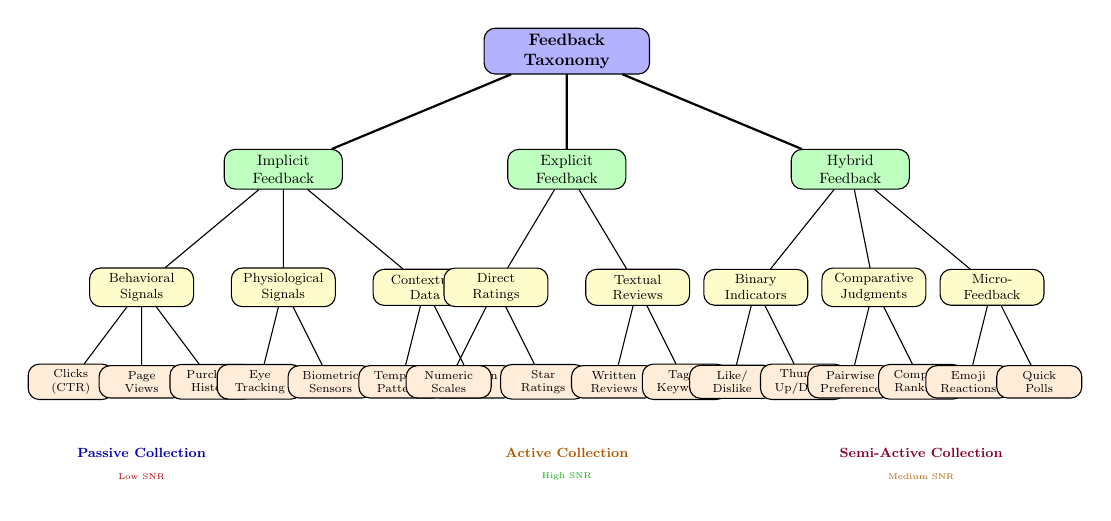
\begin{tikzpicture}[
    scale=0.60,
    transform shape,
    level 1/.style={sibling distance=8cm, level distance=2cm},
    level 2/.style={sibling distance=3.5cm, level distance=2cm},
    level 3/.style={sibling distance=1.8cm, level distance=1.8cm},
    every node/.style={draw, rectangle, rounded corners, minimum width=2.5cm, minimum height=0.7cm, align=center, font=\small},
    root/.style={fill=blue!30, font=\bfseries, minimum width=3.5cm},
    main/.style={fill=green!25},
    sub/.style={fill=yellow!20, minimum width=2.2cm, minimum height=0.6cm, font=\footnotesize},
    leaf/.style={fill=orange!15, minimum width=1.8cm, minimum height=0.5cm, font=\scriptsize}
]

% Root
\node[root] (root) at (0,0) {Feedback\\Taxonomy};

% Level 1 - Main Categories
\node[main] (implicit) at (-6,-2.5) {Implicit\\Feedback};
\node[main] (explicit) at (0,-2.5) {Explicit\\Feedback};
\node[main] (hybrid) at (6,-2.5) {Hybrid\\Feedback};

% Level 2 - Implicit subcategories
\node[sub] (behavioral) at (-9,-5) {Behavioral\\Signals};
\node[sub] (physiological) at (-6,-5) {Physiological\\Signals};
\node[sub] (contextual) at (-3,-5) {Contextual\\Data};

% Level 2 - Explicit subcategories
\node[sub] (ratings) at (-1.5,-5) {Direct\\Ratings};
\node[sub] (reviews) at (1.5,-5) {Textual\\Reviews};

% Level 2 - Hybrid subcategories
\node[sub] (binary) at (4,-5) {Binary\\Indicators};
\node[sub] (comparison) at (6.5,-5) {Comparative\\Judgments};
\node[sub] (micro) at (9,-5) {Micro-\\Feedback};

% Level 3 - Behavioral leaves
\node[leaf] (clicks) at (-10.5,-7) {Clicks\\(CTR)};
\node[leaf] (views) at (-9,-7) {Page\\Views};
\node[leaf] (purchases) at (-7.5,-7) {Purchase\\History};

% Level 3 - Physiological leaves
\node[leaf] (eye) at (-6.5,-7) {Eye\\Tracking};
\node[leaf] (biometric) at (-5,-7) {Biometric\\Sensors};

% Level 3 - Contextual leaves
\node[leaf] (temporal) at (-3.5,-7) {Temporal\\Patterns};
\node[leaf] (location) at (-2,-7) {Location\\Data};

% Level 3 - Ratings leaves
\node[leaf] (numeric) at (-2.5,-7) {Numeric\\Scales};
\node[leaf] (stars) at (-0.5,-7) {Star\\Ratings};

% Level 3 - Reviews leaves
\node[leaf] (text) at (1,-7) {Written\\Reviews};
\node[leaf] (tags) at (2.5,-7) {Tags/\\Keywords};

% Level 3 - Binary leaves
\node[leaf] (like) at (3.5,-7) {Like/\\Dislike};
\node[leaf] (thumbs) at (5,-7) {Thumbs\\Up/Down};

% Level 3 - Comparison leaves
\node[leaf] (pairwise) at (6,-7) {Pairwise\\Preference};
\node[leaf] (ranking) at (7.5,-7) {Complete\\Rankings};

% Level 3 - Micro leaves
\node[leaf] (emoji) at (8.5,-7) {Emoji\\Reactions};
\node[leaf] (quick) at (10,-7) {Quick\\Polls};

% Edges Level 1
\draw[thick] (root) -- (implicit);
\draw[thick] (root) -- (explicit);
\draw[thick] (root) -- (hybrid);

% Edges Level 2 - Implicit
\draw (implicit) -- (behavioral);
\draw (implicit) -- (physiological);
\draw (implicit) -- (contextual);

% Edges Level 2 - Explicit
\draw (explicit) -- (ratings);
\draw (explicit) -- (reviews);

% Edges Level 2 - Hybrid
\draw (hybrid) -- (binary);
\draw (hybrid) -- (comparison);
\draw (hybrid) -- (micro);

% Edges Level 3 - Behavioral
\draw (behavioral) -- (clicks);
\draw (behavioral) -- (views);
\draw (behavioral) -- (purchases);

% Edges Level 3 - Physiological
\draw (physiological) -- (eye);
\draw (physiological) -- (biometric);

% Edges Level 3 - Contextual
\draw (contextual) -- (temporal);
\draw (contextual) -- (location);

% Edges Level 3 - Ratings
\draw (ratings) -- (numeric);
\draw (ratings) -- (stars);

% Edges Level 3 - Reviews
\draw (reviews) -- (text);
\draw (reviews) -- (tags);

% Edges Level 3 - Binary
\draw (binary) -- (like);
\draw (binary) -- (thumbs);

% Edges Level 3 - Comparison
\draw (comparison) -- (pairwise);
\draw (comparison) -- (ranking);

% Edges Level 3 - Micro
\draw (micro) -- (emoji);
\draw (micro) -- (quick);

% Dimension annotations
\node[draw=none, fill=none, font=\footnotesize\bfseries, text=blue!70!black] at (-9,-8.5) {Passive Collection};
\node[draw=none, fill=none, font=\footnotesize\bfseries, text=orange!70!black] at (0,-8.5) {Active Collection};
\node[draw=none, fill=none, font=\footnotesize\bfseries, text=purple!70!black] at (7.5,-8.5) {Semi-Active Collection};

% Quality indicators
\node[draw=none, fill=none, font=\tiny, text=red!70!black] at (-9,-9) {Low SNR};
\node[draw=none, fill=none, font=\tiny, text=green!70!black] at (0,-9) {High SNR};
\node[draw=none, fill=none, font=\tiny, text=orange!70!black] at (7.5,-9) {Medium SNR};

\end{tikzpicture}
\caption{Comprehensive hierarchical taxonomy of feedback types in recommender systems. The tree illustrates three primary feedback categories (Implicit, Explicit, Hybrid), their subcategories organized by collection mechanism, and specific instantiations at the leaf level. Color coding indicates collection mechanism: passive (blue), active (orange), and semi-active (purple). Signal-to-noise ratio (SNR) annotations indicate typical reliability levels for each category. This taxonomy enables systematic categorization and comparison of feedback across diverse recommendation domains and application contexts.}
\Description{A hierarchical tree diagram showing feedback taxonomy with three levels. The root node splits into Implicit, Explicit, and Hybrid feedback. Implicit branches into Behavioral Signals, Physiological Signals, and Contextual Data with specific examples like clicks, eye tracking, and temporal patterns. Explicit branches into Direct Ratings and Textual Reviews with examples like star ratings and written reviews. Hybrid branches into Binary Indicators, Comparative Judgments, and Micro-Feedback with examples like thumbs up/down and emoji reactions.}
\label{fig:feedback_taxonomy_tree}
\end{figure*}

\subsubsection{Dimension 1: Collection Mechanism}
This dimension characterizes how feedback is obtained from users, spanning three primary categories along a continuum from fully automated to explicitly intentional.

\textbf{Passive Collection} encompasses feedback automatically captured without requiring user intention or awareness. Behavioral tracking captures user interactions including clicks, page views, and navigation patterns that naturally occur during system use. Physiological signals leverage biometric sensors to measure eye tracking patterns, galvanic skin responses, heart rate variations, and other involuntary responses that reveal affective states and attention. Environmental context data encompasses location information, temporal patterns, device characteristics, and ambient conditions that provide situational awareness without explicit user input.

\textbf{Active Collection} requires deliberate user action to provide feedback, typically involving conscious evaluation and expression of preferences. Direct ratings ask users to provide numerical scores or categorical assessments that explicitly quantify their preferences for items. Comparative judgments elicit pairwise preferences or complete rankings that reveal relative preferences through structured comparisons. Textual feedback includes written reviews, comments, and explanations that provide rich, nuanced preference information along with supporting rationale and context.

\textbf{Semi-Active Collection} occupies the middle ground, requiring minimal user effort while still involving intentional feedback provision. Binary indicators like thumbs up/down or like/dislike buttons provide simple approval signals with minimal cognitive burden. Implicit confirmations capture decisions to accept or reject system recommendations, revealing preferences through choice behavior. Micro-feedback mechanisms solicit quick satisfaction indicators through lightweight interactions that interrupt user flow minimally.

\subsubsection{Dimension 2: Signal Quality and Noise Characteristics}

\textbf{Signal-to-Noise Ratio} quantifies the reliability with which preferences can be inferred from feedback signals. High SNR feedback like direct ratings provides clear semantic meaning with minimal ambiguity about user preferences. Medium SNR signals such as purchase behavior contain some ambiguity, as purchases may reflect factors beyond preference including necessity, price sensitivity, or gift-giving. Low SNR data like click-through behavior exhibits high noise levels, as clicks may result from curiosity, accidental interaction, or interface design rather than genuine interest.

\textbf{Confidence Indicators} provide measures of feedback reliability across multiple assessment approaches. User-provided confidence captures self-assessed certainty ratings that users supply alongside their primary feedback. Behavioral confidence is inferred from action characteristics such as dwell time, repeat interactions, or interaction intensity that suggest stronger or weaker preference signals. Statistical confidence derives from pattern consistency across multiple observations, identifying reliable signals through temporal stability and cross-contextual agreement.

\subsubsection{Dimension 3: Temporal Characteristics}

\textbf{Feedback Latency} describes the time delay between item experience and feedback provision, with significant implications for signal quality. Real-time feedback captures immediate behavioral responses that occur during or immediately following item consumption. Short-term feedback arrives within hours or days of the experience, reflecting deliberate but relatively prompt evaluation. Long-term feedback involves delayed evaluations provided after extended use or reflection, potentially offering deeper insight but risking memory decay and context loss.

\textbf{Temporal Persistence} characterizes the stability of feedback signals over time, revealing the nature of underlying preferences. Stable feedback exhibits consistent preferences across extended periods, simplifying long-term modeling and prediction. Evolving feedback demonstrates gradually changing preferences driven by learning, life stage transitions, or shifting interests that require adaptive models. Volatile feedback shows rapidly fluctuating preferences influenced by contextual factors, mood variations, or exploratory behavior that challenges prediction algorithms.

\subsubsection{Dimension 4: Cognitive Load and User Effort}

\textbf{Effort Requirements} quantify the cognitive and physical costs users must bear to provide feedback. Zero-effort feedback relies on automatic behavioral tracking that imposes no burden beyond normal system use. Minimal-effort interactions like single-click buttons require simple motor actions with negligible cognitive processing. Moderate-effort mechanisms including rating scales and binary choices demand some conscious evaluation and decision-making. High-effort feedback such as detailed reviews and explanations requires substantial cognitive investment in articulation and composition.

\textbf{User Awareness} captures the extent to which users consciously recognize they are providing feedback. Unconscious feedback arises from automatic behavioral capture that users may not realize is being collected or analyzed. Semi-conscious feedback occurs when users are aware of data collection but it is not their primary focus during interaction. Conscious feedback involves deliberate, intentional feedback provision where users explicitly aim to communicate their preferences to the system.

\subsubsection{Dimension 5: Privacy and Sensitivity}

\textbf{Privacy Implications} assess the sensitivity of feedback data and associated sharing comfort levels. Public feedback like product ratings can be openly shared without privacy concerns, often intentionally made visible to other users. Semi-private data such as platform-specific purchase histories remain within organizational boundaries but are not publicly disclosed. Private feedback including detailed browsing histories contains sensitive behavioral patterns that users expect will be protected from disclosure. Highly sensitive data involving personal health, financial, or intimate preference information demands the strongest privacy protections and consent practices.

\textbf{Consent Requirements} specify the level of user agreement necessary for ethical feedback collection. Implicit consent assumes agreement through general platform use, typically documented in terms of service agreements. Explicit consent requires clear, specific agreement for particular data collection practices, often mandated by privacy regulations. Granular consent provides fine-grained user control over different data types and uses, empowering users to make nuanced privacy decisions that reflect their individual comfort levels and trust in the platform.

\begin{figure}[ht]
\centering
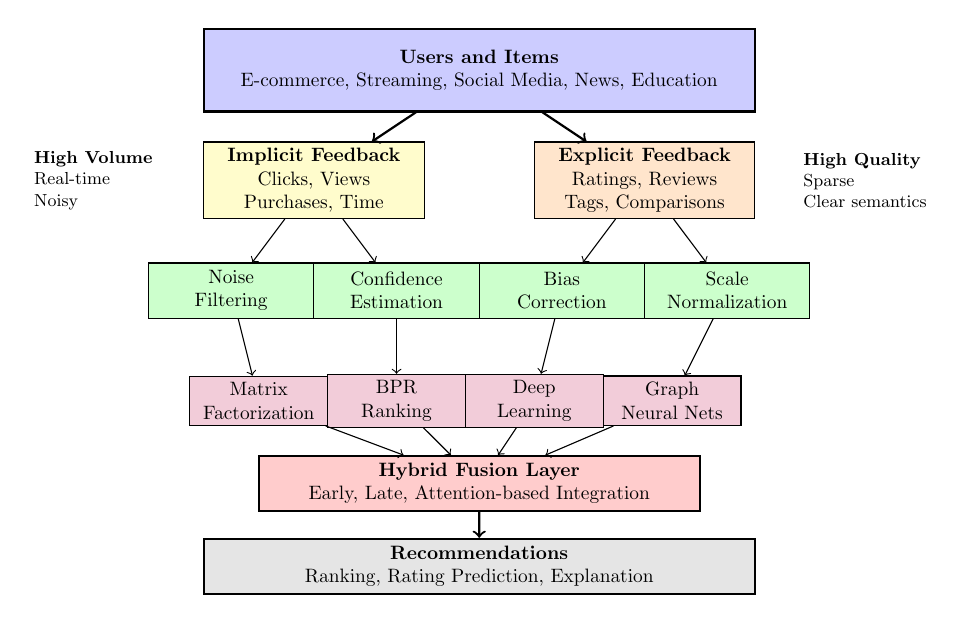
\begin{tikzpicture}[scale=0.7, transform shape]
    % User layer
    \node[rectangle, draw, thick, fill=blue!20, minimum width=10cm, minimum height=1.5cm, align=center] (users) at (0,8) {\textbf{Users and Items}\\E-commerce, Streaming, Social Media, News, Education};
    
    % Feedback collection layer
    \node[rectangle, draw, fill=yellow!20, minimum width=4cm, minimum height=1.2cm, align=center] (implicit) at (-3,6) {\textbf{Implicit Feedback}\\Clicks, Views\\Purchases, Time};
    \node[rectangle, draw, fill=orange!20, minimum width=4cm, minimum height=1.2cm, align=center] (explicit) at (3,6) {\textbf{Explicit Feedback}\\Ratings, Reviews\\Tags, Comparisons};
    
    % Processing layer
    \node[rectangle, draw, fill=green!20, minimum width=3cm, minimum height=1cm, align=center] (preprocess1) at (-4.5,4) {Noise\\Filtering};
    \node[rectangle, draw, fill=green!20, minimum width=3cm, minimum height=1cm, align=center] (preprocess2) at (-1.5,4) {Confidence\\Estimation};
    \node[rectangle, draw, fill=green!20, minimum width=3cm, minimum height=1cm, align=center] (preprocess3) at (1.5,4) {Bias\\Correction};
    \node[rectangle, draw, fill=green!20, minimum width=3cm, minimum height=1cm, align=center] (preprocess4) at (4.5,4) {Scale\\Normalization};
    
    % Algorithm layer
    \node[rectangle, draw, fill=purple!20, minimum width=2.5cm, minimum height=0.8cm, align=center] (mf) at (-4,2) {Matrix\\Factorization};
    \node[rectangle, draw, fill=purple!20, minimum width=2.5cm, minimum height=0.8cm, align=center] (bpr) at (-1.5,2) {BPR\\Ranking};
    \node[rectangle, draw, fill=purple!20, minimum width=2.5cm, minimum height=0.8cm, align=center] (deep) at (1,2) {Deep\\Learning};
    \node[rectangle, draw, fill=purple!20, minimum width=2.5cm, minimum height=0.8cm, align=center] (graph) at (3.5,2) {Graph\\Neural Nets};
    
    % Fusion layer
    \node[rectangle, draw, thick, fill=red!20, minimum width=8cm, minimum height=1cm, align=center] (fusion) at (0,0.5) {\textbf{Hybrid Fusion Layer}\\Early, Late, Attention-based Integration};
    
    % Output layer
    \node[rectangle, draw, thick, fill=gray!20, minimum width=10cm, minimum height=1cm, align=center] (output) at (0,-1) {\textbf{Recommendations}\\Ranking, Rating Prediction, Explanation};
    
    % Arrows
    \draw[thick, ->] (users) -- (implicit);
    \draw[thick, ->] (users) -- (explicit);
    \draw[->] (implicit) -- (preprocess1);
    \draw[->] (implicit) -- (preprocess2);
    \draw[->] (explicit) -- (preprocess3);
    \draw[->] (explicit) -- (preprocess4);
    \draw[->] (preprocess1) -- (mf);
    \draw[->] (preprocess2) -- (bpr);
    \draw[->] (preprocess3) -- (deep);
    \draw[->] (preprocess4) -- (graph);
    \draw[->] (mf) -- (fusion);
    \draw[->] (bpr) -- (fusion);
    \draw[->] (deep) -- (fusion);
    \draw[->] (graph) -- (fusion);
    \draw[thick, ->] (fusion) -- (output);
    
    % Side annotations
    \node[align=left, font=\small] at (-7,6) {\textbf{High Volume}\\Real-time\\Noisy};
    \node[align=left, font=\small] at (7,6) {\textbf{High Quality}\\Sparse\\Clear semantics};
    
\end{tikzpicture}
\caption{Unified System Architecture for Feedback-Aware Recommender Systems}
\Description{A system architecture diagram showing the flow from user-item interactions through implicit and explicit feedback collection, then through preprocessing layers (implicit features and explicit features), into modeling algorithms (Matrix Factorization, BPR Ranking, Deep Learning, and Graph Neural Networks), combined through a Hybrid Fusion Layer using early, late, or attention-based integration, and finally producing recommendations with ranking, rating prediction, and explanations.}
\label{fig:system_architecture}
\end{figure}

Figure~\ref{fig:system_architecture} presents our unified architecture that systematically processes both implicit and explicit feedback through specialized preprocessing, algorithmic modeling, and fusion components.

\begin{figure*}[ht]
\centering
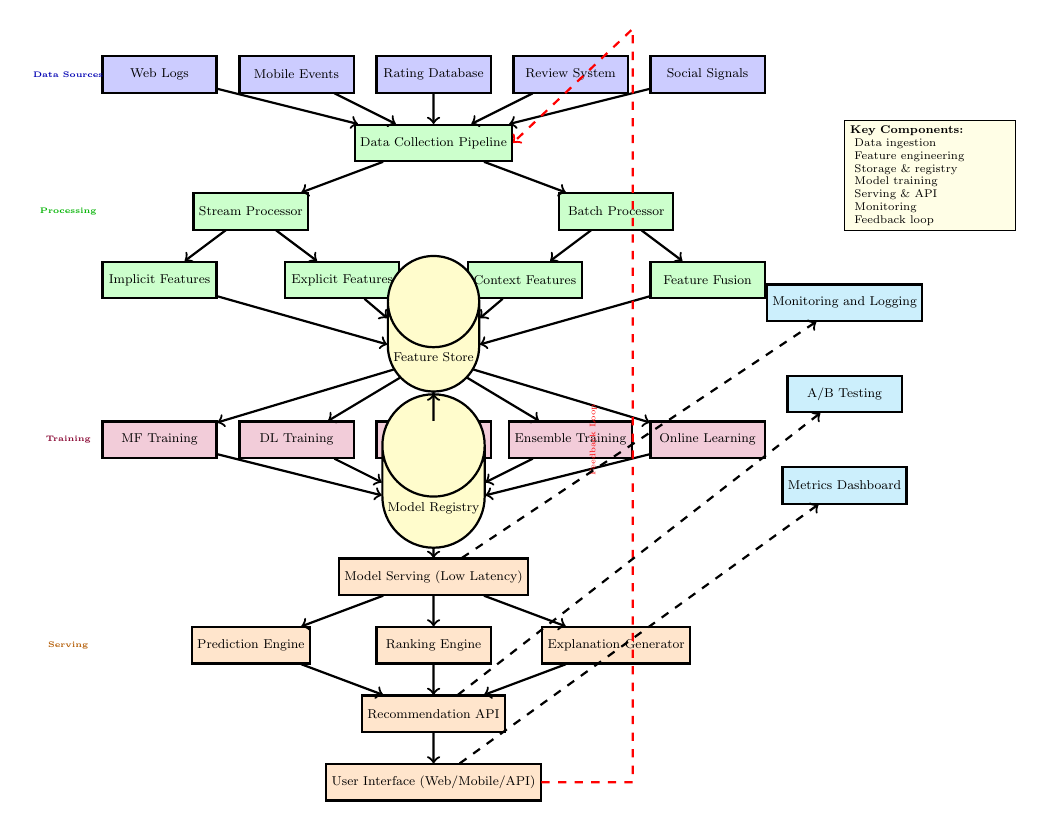
\begin{tikzpicture}[
    scale=0.58,
    transform shape,
    box/.style={rectangle, draw, thick, minimum width=2.5cm, minimum height=0.8cm, align=center, font=\footnotesize},
    data/.style={box, fill=blue!20},
    process/.style={box, fill=green!20},
    model/.style={box, fill=purple!20},
    output/.style={box, fill=orange!20},
    storage/.style={cylinder, draw, thick, minimum width=2cm, minimum height=1cm, shape border rotate=90, fill=yellow!20, font=\footnotesize}
]

% Top: Data Sources
\node[data] (web) at (0,10) {Web Logs};
\node[data] (mobile) at (3,10) {Mobile Events};
\node[data] (ratings) at (6,10) {Rating Database};
\node[data] (reviews) at (9,10) {Review System};
\node[data] (social) at (12,10) {Social Signals};

% Data Collection Layer
\node[process] (collector) at (6,8.5) {Data Collection Pipeline};
\draw[thick, ->] (web) -- (collector);
\draw[thick, ->] (mobile) -- (collector);
\draw[thick, ->] (ratings) -- (collector);
\draw[thick, ->] (reviews) -- (collector);
\draw[thick, ->] (social) -- (collector);

% Stream Processing
\node[process] (stream) at (2,7) {Stream Processor};
\node[process] (batch) at (10,7) {Batch Processor};
\draw[thick, ->] (collector) -- (stream);
\draw[thick, ->] (collector) -- (batch);

% Feature Engineering
\node[process] (implicit_fe) at (0,5.5) {Implicit Features};
\node[process] (explicit_fe) at (4,5.5) {Explicit Features};
\node[process] (context_fe) at (8,5.5) {Context Features};
\node[process] (fusion_fe) at (12,5.5) {Feature Fusion};

\draw[thick, ->] (stream) -- (implicit_fe);
\draw[thick, ->] (stream) -- (explicit_fe);
\draw[thick, ->] (batch) -- (context_fe);
\draw[thick, ->] (batch) -- (fusion_fe);

% Storage Layer
\node[storage] (feature_store) at (6,3.8) {Feature Store};
\draw[thick, ->] (implicit_fe) -- (feature_store);
\draw[thick, ->] (explicit_fe) -- (feature_store);
\draw[thick, ->] (context_fe) -- (feature_store);
\draw[thick, ->] (fusion_fe) -- (feature_store);

% Model Training Pipeline
\node[model] (mf_train) at (0,2) {MF Training};
\node[model] (dl_train) at (3,2) {DL Training};
\node[model] (gnn_train) at (6,2) {GNN Training};
\node[model] (ensemble) at (9,2) {Ensemble Training};
\node[model] (online_learn) at (12,2) {Online Learning};

\draw[thick, ->] (feature_store) -- (mf_train);
\draw[thick, ->] (feature_store) -- (dl_train);
\draw[thick, ->] (feature_store) -- (gnn_train);
\draw[thick, ->] (feature_store) -- (ensemble);
\draw[thick, ->] (feature_store) -- (online_learn);

% Model Registry
\node[storage] (model_registry) at (6,0.5) {Model Registry};
\draw[thick, ->] (mf_train) -- (model_registry);
\draw[thick, ->] (dl_train) -- (model_registry);
\draw[thick, ->] (gnn_train) -- (model_registry);
\draw[thick, ->] (ensemble) -- (model_registry);
\draw[thick, ->] (online_learn) -- (model_registry);

% Serving Layer
\node[output] (serving) at (6,-1) {Model Serving (Low Latency)};
\draw[thick, ->] (model_registry) -- (serving);

% Prediction & Ranking
\node[output] (prediction) at (2,-2.5) {Prediction Engine};
\node[output] (ranking) at (6,-2.5) {Ranking Engine};
\node[output] (explanation) at (10,-2.5) {Explanation Generator};

\draw[thick, ->] (serving) -- (prediction);
\draw[thick, ->] (serving) -- (ranking);
\draw[thick, ->] (serving) -- (explanation);

% API Layer
\node[output] (api) at (6,-4) {Recommendation API};
\draw[thick, ->] (prediction) -- (api);
\draw[thick, ->] (ranking) -- (api);
\draw[thick, ->] (explanation) -- (api);

% User Interface
\node[output] (ui) at (6,-5.5) {User Interface (Web/Mobile/API)};
\draw[thick, ->] (api) -- (ui);

% Feedback Loop
\draw[thick, ->, dashed, red] (ui.east) -- ++(2,0) -- ++(0,16.5) -- (collector.east);
\node[draw=none, fill=none, font=\tiny, text=red, rotate=90] at (9.5,2) {Feedback Loop};

% Monitoring & Evaluation
\node[process, fill=cyan!20] (monitoring) at (15,5) {Monitoring and Logging};
\node[process, fill=cyan!20] (ab_test) at (15,3) {A/B Testing};
\node[process, fill=cyan!20] (metrics) at (15,1) {Metrics Dashboard};

\draw[thick, ->, dashed] (serving) -- (monitoring);
\draw[thick, ->, dashed] (api) -- (ab_test);
\draw[thick, ->, dashed] (ui) -- (metrics);

% Annotations
\node[draw=none, fill=none, font=\tiny\bfseries, text=blue!70!black] at (-2,10) {Data Sources};
\node[draw=none, fill=none, font=\tiny\bfseries, text=green!70!black] at (-2,7) {Processing};
\node[draw=none, fill=none, font=\tiny\bfseries, text=purple!70!black] at (-2,2) {Training};
\node[draw=none, fill=none, font=\tiny\bfseries, text=orange!70!black] at (-2,-2.5) {Serving};

% Key Components Box
\node[draw, rectangle, fill=yellow!10, align=left, font=\scriptsize, anchor=north west, text width=3.5cm] at (15,9) {
    \textbf{Key Components:}\\
    \textcolor{blue}{$\blacksquare$} Data ingestion\\
    \textcolor{green}{$\blacksquare$} Feature engineering\\
    \textcolor{yellow!70!black}{$\blacksquare$} Storage \& registry\\
    \textcolor{purple}{$\blacksquare$} Model training\\
    \textcolor{orange}{$\blacksquare$} Serving \& API\\
    \textcolor{cyan}{$\blacksquare$} Monitoring\\
    \textcolor{red}{$\blacksquare$} Feedback loop
};

\end{tikzpicture}
\caption{Complete end-to-end production architecture for implicit-explicit hybrid recommender systems. The diagram illustrates the full data flow from multiple sources (web logs, mobile events, ratings, reviews, social signals) through real-time stream and batch processing pipelines, feature engineering and storage, distributed model training (matrix factorization, deep learning, graph neural networks, ensemble methods, online learning), model registry and serving infrastructure, prediction and ranking engines, API layer, and user interface. The red dashed line shows the critical feedback loop that captures new user interactions to continuously improve the system. Cyan components represent monitoring, A/B testing, and metrics infrastructure for production system health and performance evaluation.}
\Description{A comprehensive system architecture diagram showing the end-to-end flow from multiple data sources through processing pipelines, model training, serving infrastructure, to user interface. The architecture includes data collection from web logs, mobile events, ratings, reviews, and social signals; real-time and batch processing pipelines; feature storage in key-value and vector stores; distributed training of multiple model types (matrix factorization, deep learning, graph neural networks, ensemble methods, online learning); model registry and serving infrastructure; prediction and ranking engines; API layer; and user interface, with a feedback loop returning user interactions to the system for continuous improvement.}
\label{fig:end_to_end_architecture}
\end{figure*}

Figure~\ref{fig:end_to_end_architecture} presents the complete production system architecture, illustrating how modern recommendation platforms integrate diverse feedback sources through sophisticated data engineering, distributed training, and low-latency serving infrastructure.

\subsection{Algorithmic Framework Analysis}

We systematically analyze algorithmic approaches across feedback types, organizing them into fundamental paradigms that reveal underlying principles and trade-offs.

\subsubsection{Explicit Feedback Algorithms}

\textbf{Matrix Factorization Approaches}
For explicit feedback matrix $R \in \mathbb{R}^{m \times n}$ with users $m$ and items $n$:

\begin{equation}
\min_{P,Q} \sum_{(u,i) \in \Omega} (r_{ui} - p_u^T q_i)^2 + \lambda(||P||_F^2 + ||Q||_F^2)
\end{equation}

where $P \in \mathbb{R}^{m \times k}$ and $Q \in \mathbb{R}^{n \times k}$ are user and item latent factor matrices, $\Omega$ is the set of observed ratings, and $\lambda$ is the regularization parameter.

\textbf{Neighborhood-Based Methods}
User-based collaborative filtering predicts ratings as:

\begin{equation}
\hat{r}_{ui} = \bar{r}_u + \frac{\sum_{v \in N(u)} sim(u,v) \cdot (r_{vi} - \bar{r}_v)}{\sum_{v \in N(u)} |sim(u,v)|}
\end{equation}

where $N(u)$ represents the neighborhood of user $u$, $sim(u,v)$ is user similarity, and $\bar{r}_u$ is the average rating for user $u$.

\subsubsection{Implicit Feedback Algorithms}

\textbf{Weighted Matrix Factorization}
For implicit feedback, Hu et al.~\cite{hu2008collaborative} proposed:

\begin{equation}
\min_{P,Q} \sum_{u,i} c_{ui}(p_{ui} - p_u^T q_i)^2 + \lambda(||P||_F^2 + ||Q||_F^2)
\end{equation}

where $c_{ui}$ represents confidence in the observation, $p_{ui} = 1$ if user $u$ interacted with item $i$, and $p_{ui} = 0$ otherwise.

\textbf{Bayesian Personalized Ranking}
BPR optimizes for ranking by maximizing:

\begin{equation}
\prod_{u,i,j} \sigma(\hat{r}_{ui} - \hat{r}_{uj})
\end{equation}

where $\sigma$ is the sigmoid function, and $(u,i,j)$ represents training triplets where user $u$ prefers item $i$ over item $j$.

\subsubsection{Deep Learning Approaches}

\textbf{Neural Collaborative Filtering}
NCF generalizes matrix factorization using neural networks:

\begin{equation}
\hat{r}_{ui} = f(P^T v_u^U, Q^T v_i^I | P, Q, \Theta_f)
\end{equation}

where $v_u^U$ and $v_i^I$ are one-hot encodings, $P$ and $Q$ are embedding matrices, and $\Theta_f$ represents neural network parameters.

\textbf{Autoencoder-Based Methods}
AutoRec learns user/item representations by reconstructing rating vectors:

\begin{equation}
\min_{\Theta} \sum_{u=1}^m ||r^{(u)} - f(r^{(u)}; \Theta)||_2^2 + \frac{\lambda}{2}||\Theta||_F^2
\end{equation}

where $f(\cdot; \Theta)$ is the autoencoder function with parameters $\Theta$.

\subsubsection{Hybrid Integration Strategies}

\textbf{Early Fusion}: Combine features before model training
\begin{equation}
\hat{r}_{ui} = f([x_{ui}^{impl}; x_{ui}^{expl}]; \Theta)
\end{equation}

\textbf{Late Fusion}: Combine predictions from separate models
\begin{equation}
\hat{r}_{ui} = \alpha \cdot f^{impl}(x_{ui}^{impl}) + (1-\alpha) \cdot f^{expl}(x_{ui}^{expl})
\end{equation}

\textbf{Attention-Based Fusion}: Learn dynamic combination weights
\begin{equation}
\hat{r}_{ui} = \sum_k \alpha_k \cdot f^{(k)}(x_{ui}^{(k)})
\end{equation}

where $\alpha_k = \text{softmax}(g(x_{ui}^{(k)}))$ and $g(\cdot)$ is an attention network.

\subsection{Comparative Analysis Framework}

To systematically evaluate different feedback types and algorithmic approaches, we present comprehensive comparison tables that highlight key characteristics, trade-offs, and performance considerations.

\subsubsection{Feedback Type Characteristics}
Table~\ref{tab:feedback_comparison} provides a detailed comparison of implicit and explicit feedback across multiple dimensions, enabling practitioners to make informed design decisions.

\begin{table}[ht]
\centering
\caption{Comprehensive Comparison of Feedback Types}
\label{tab:feedback_comparison}
\small
\begin{tabular}{@{}lccc@{}}
\toprule
\textbf{Characteristic} & \textbf{Implicit} & \textbf{Explicit} & \textbf{Hybrid} \\
\midrule
\multicolumn{4}{l}{\textbf{Data Collection}} \\
User Effort & None & High & Medium \\
Collection Volume & Very High & Low & High \\
Real-time Availability & Yes & No & Partial \\
Scalability & Excellent & Poor & Good \\
\midrule
\multicolumn{4}{l}{\textbf{Signal Quality}} \\
Preference Clarity & Low & High & Medium \\
Noise Level & High & Low & Medium \\
Confidence Level & Variable & High & Variable \\
Semantic Richness & Low & High & Medium \\
\midrule
\multicolumn{4}{l}{\textbf{Algorithmic Challenges}} \\
Negative Examples & Difficult & Available & Partial \\
Cold Start Problem & Severe & Moderate & Moderate \\
Sparsity Issues & Low & High & Medium \\
Computational Cost & Medium & Low & High \\
\midrule
\multicolumn{4}{l}{\textbf{System Performance}} \\
Training Speed & Fast & Medium & Slow \\
Inference Speed & Fast & Fast & Medium \\
Memory Requirements & Medium & Low & High \\
Model Complexity & Medium & Low & High \\
\midrule
\multicolumn{4}{l}{\textbf{Business Considerations}} \\
User Experience & Seamless & Intrusive & Balanced \\
Feedback Loop & Immediate & Delayed & Mixed \\
Privacy Concerns & High & Low & Medium \\
Implementation Cost & Low & Medium & High \\
\bottomrule
\end{tabular}
\end{table}

\subsubsection{Algorithmic Approach Comparison}
Table~\ref{tab:algorithm_comparison} summarizes the characteristics of major algorithmic families for different feedback types.

\begin{table}[ht]
\centering
\caption{Algorithmic Approaches by Feedback Type}
\label{tab:algorithm_comparison}
\small
\begin{tabular}{@{}lccccc@{}}
\toprule
\textbf{Algorithm} & \textbf{Implicit} & \textbf{Explicit} & \textbf{Complexity} & \textbf{Scalability} & \textbf{Performance} \\
\midrule
Neighborhood-based CF & Good & Excellent & $O(n^2)$ & Poor & Medium \\
Matrix Factorization & Excellent & Excellent & $O(nk)$ & Good & High \\
Deep Neural Networks & Excellent & Good & $O(nd)$ & Medium & High \\
BPR/Ranking Methods & Excellent & Poor & $O(n \log n)$ & Good & High \\
Graph-based Methods & Good & Good & $O(n^{1.5})$ & Medium & High \\
Autoencoder-based & Good & Excellent & $O(nd)$ & Medium & Medium \\
Attention Mechanisms & Good & Good & $O(n^2 d)$ & Poor & High \\
\midrule
\multicolumn{6}{l}{\textbf{Legend:} $n$ = users/items, $k$ = latent factors, $d$ = network depth} \\
\bottomrule
\end{tabular}
\end{table}

\begin{figure}[ht]
\centering
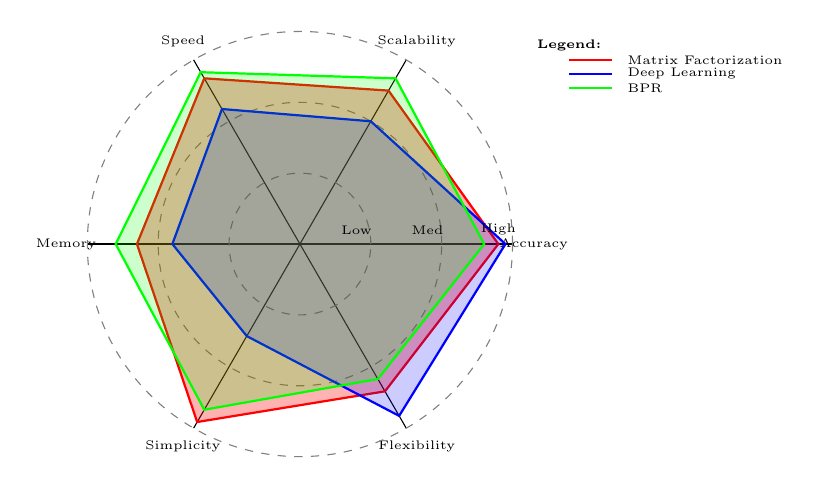
\begin{tikzpicture}[scale=0.9, transform shape]
    % Create a radar chart for algorithm comparison
    \def\n{6}
    \def\radius{3}
    
    % Draw axes - ADJUSTED LABEL POSITIONING
    \foreach \i in {0,...,5} {
        \draw (0,0) -- (\i*60:\radius);
        \node at (\i*60:\radius+0.3) [anchor=center, font=\tiny] {
            \ifcase\i Accuracy\or Scalability\or Speed\or Memory\or Simplicity\or Flexibility\fi
        };
    }
    
    % Draw concentric circles
    \foreach \r in {1,2,3} {
        \draw[gray, dashed] (0,0) circle (\r);
    }
    
    % Algorithm 1: Matrix Factorization
    \coordinate (mf0) at (0*60:2.8);
    \coordinate (mf1) at (1*60:2.5);
    \coordinate (mf2) at (2*60:2.7);
    \coordinate (mf3) at (3*60:2.3);
    \coordinate (mf4) at (4*60:2.9);
    \coordinate (mf5) at (5*60:2.4);
    \draw[red, thick] (mf0) -- (mf1) -- (mf2) -- (mf3) -- (mf4) -- (mf5) -- cycle;
    \fill[red, opacity=0.3] (mf0) -- (mf1) -- (mf2) -- (mf3) -- (mf4) -- (mf5) -- cycle;
    
    % Algorithm 2: Deep Learning
    \coordinate (dl0) at (0*60:2.9);
    \coordinate (dl1) at (1*60:2.0);
    \coordinate (dl2) at (2*60:2.2);
    \coordinate (dl3) at (3*60:1.8);
    \coordinate (dl4) at (4*60:1.5);
    \coordinate (dl5) at (5*60:2.8);
    \draw[blue, thick] (dl0) -- (dl1) -- (dl2) -- (dl3) -- (dl4) -- (dl5) -- cycle;
    \fill[blue, opacity=0.2] (dl0) -- (dl1) -- (dl2) -- (dl3) -- (dl4) -- (dl5) -- cycle;
    
    % Algorithm 3: BPR
    \coordinate (bpr0) at (0*60:2.6);
    \coordinate (bpr1) at (1*60:2.7);
    \coordinate (bpr2) at (2*60:2.8);
    \coordinate (bpr3) at (3*60:2.6);
    \coordinate (bpr4) at (4*60:2.7);
    \coordinate (bpr5) at (5*60:2.2);
    \draw[green, thick] (bpr0) -- (bpr1) -- (bpr2) -- (bpr3) -- (bpr4) -- (bpr5) -- cycle;
    \fill[green, opacity=0.2] (bpr0) -- (bpr1) -- (bpr2) -- (bpr3) -- (bpr4) -- (bpr5) -- cycle;
    
    % Legend - REPOSITIONED TO AVOID COLLISION
    \node[font=\tiny] at (3.8,2.8) {\textbf{Legend:}};
    \draw[red, thick] (3.8,2.6) -- (4.4,2.6);
    \node[font=\tiny, anchor=west] at (4.5,2.6) {Matrix Factorization};
    \draw[blue, thick] (3.8,2.4) -- (4.4,2.4);
    \node[font=\tiny, anchor=west] at (4.5,2.4) {Deep Learning};
    \draw[green, thick] (3.8,2.2) -- (4.4,2.2);
    \node[font=\tiny, anchor=west] at (4.5,2.2) {BPR};
    
    % Scale labels
    \node[font=\tiny] at (0.8,0.2) {Low};
    \node[font=\tiny] at (1.8,0.2) {Med};
    \node[font=\tiny] at (2.8,0.2) {High};
    
\end{tikzpicture}
\caption{Algorithmic Performance Comparison Across Multiple Dimensions}
\Description{A radar/spider chart comparing six recommendation algorithm families (Collaborative Filtering, Content-Based, Matrix Factorization, Deep Learning, Graph Neural Networks, LLM-Based) across five performance dimensions (Accuracy, Scalability, Interpretability, Cold-Start, Diversity) on a 0-10 scale. The chart reveals that Matrix Factorization and Deep Learning excel in accuracy and scalability, while Content-Based methods provide better interpretability, and Graph Neural Networks show balanced performance across dimensions.}
\label{fig:algorithm_performance}
\end{figure}

Figure~\ref{fig:algorithm_performance} provides a multi-dimensional comparison of major algorithmic approaches, illustrating their relative strengths and trade-offs across key performance criteria.

\subsection{Complexity Analysis and Trade-offs}

\subsubsection{Computational Complexity}
We analyze the computational requirements for different algorithmic approaches:

\textbf{Matrix Factorization}:
\begin{itemize}
    \item Training: $O(|\Omega| \cdot k \cdot t)$ where $t$ is iterations
    \item Inference: $O(k)$ per prediction
    \item Space: $O((m+n) \cdot k)$
\end{itemize}

\textbf{Deep Neural Networks}:
\begin{itemize}
    \item Training: $O(|\Omega| \cdot d \cdot t)$ where $d$ is network complexity
    \item Inference: $O(d)$ per prediction
    \item Space: $O(d)$ for parameters
\end{itemize}

\subsubsection{Feedback-Specific Considerations}

\textbf{Implicit Feedback Challenges}:
\begin{itemize}
    \item \textit{Confidence estimation}: Determining reliability of implicit signals
    \item \textit{Negative sampling}: Generating negative examples for training
    \item \textit{Temporal modeling}: Capturing evolving preferences from behavior
\end{itemize}

\textbf{Explicit Feedback Challenges}:
\begin{itemize}
    \item \textit{Sparsity handling}: Dealing with limited rating coverage
    \item \textit{Bias correction}: Addressing selection and rating biases
    \item \textit{Scale consistency}: Normalizing across different rating scales
\end{itemize}

\textbf{Hybrid System Challenges}:
\begin{itemize}
    \item \textit{Modality alignment}: Ensuring compatible representations
    \item \textit{Conflict resolution}: Handling contradictory signals
    \item \textit{Dynamic weighting}: Adapting combination strategies over time
\end{itemize}

\subsection{Theoretical Analysis and Guarantees}

\subsubsection{Convergence Properties}
We analyze convergence guarantees for different algorithmic approaches:

\textbf{Matrix Factorization}: Under appropriate regularization, alternating least squares converges to a local minimum with rate $O(1/t)$.

\textbf{BPR Optimization}: Stochastic gradient descent for BPR converges with rate $O(1/\sqrt{t})$ under standard assumptions.

\subsubsection{Generalization Bounds}
For matrix factorization with $k$ latent factors and $n$ training samples:

\begin{equation}
R(f) \leq \hat{R}(f) + O\left(\sqrt{\frac{k \log n}{n}}\right)
\end{equation}

where $R(f)$ is the true risk and $\hat{R}(f)$ is the empirical risk.

\subsection{Practical Implementation Considerations}

\subsubsection{Scalability Strategies}
\begin{itemize}
    \item \textbf{Distributed computing}: Parallelization across multiple machines
    \item \textbf{Online learning}: Incremental updates with streaming data
    \item \textbf{Approximation methods}: Randomized algorithms for large-scale systems
    \item \textbf{Caching strategies}: Efficient storage and retrieval of recommendations
\end{itemize}

\subsubsection{System Architecture Patterns}
\begin{itemize}
    \item \textbf{Lambda architecture}: Separate batch and stream processing pipelines
    \item \textbf{Microservices}: Modular services for different feedback types
    \item \textbf{Feature stores}: Centralized feature management and serving
    \item \textbf{Model serving}: Low-latency prediction infrastructure
\end{itemize}

This unified framework provides the theoretical foundation for systematic analysis of feedback mechanisms and guides the development of optimal hybrid systems that leverage the complementary strengths of different feedback types.

\paragraph{Qualitative Explicit Feedback}
\begin{itemize}
    \item \textbf{Textual reviews}: Written opinions, critiques, and detailed feedback.
    \item \textbf{Tags and categories}: User-assigned labels and classifications.
    \item \textbf{Feature ratings}: Specific aspect ratings (e.g., "sound quality: 4/5, plot: 3/5").
    \item \textbf{Comparative feedback}: Direct comparisons between items or against expectations.
\end{itemize}

\paragraph{Interactive Explicit Feedback}
\begin{itemize}
    \item \textbf{Conversational feedback}: Dialogue-based preference elicitation through chat interfaces.
    \item \textbf{Preference surveys}: Structured questionnaires and preference profiling.
    \item \textbf{Active learning queries}: System-initiated questions to clarify user preferences.
\end{itemize}

\subsection{Feedback Properties and Characteristics}

Feedback types exhibit distinct properties that influence their utility, reliability, and modeling requirements. Understanding these properties is crucial for designing appropriate algorithms and evaluation metrics.

\subsubsection{Data Abundance and Collection Dynamics}

\begin{table}[h]
\centering
\tiny
\caption{Comparative Analysis of Feedback Properties}
\label{tab:feedback_properties_detailed}
\begin{tabular}{@{}lcccc@{}}
\toprule
Property & Implicit & Explicit & Hybrid & Key Implications \\
\midrule
Data Volume & VHigh & Low-Mod & High & Scalability trade-offs \\
Collection Cost & $\sim$0 & High & Variable & Economic consider. \\
Temporal Res. & Real-time & Delayed & Mixed & Adaptation speed \\
Semantic Clarity & Low & High & Moderate & Interp. complexity \\
Noise Level & High & Low-Mod & Moderate & Signal proc. needs \\
Sparsity & Extreme & Variable & Reduced & Matrix completion \\
Bias Types & Behavior & Self-sel. & Compound & Fairness needs \\
Privacy & Moderate & High & High & Regulatory compl. \\
User Burden & None & High & Moderate & Engagement strat. \\
Context Rich. & High & Low-Mod & High & Personalization \\
\bottomrule
\end{tabular}
\end{table}

\subsubsection{Noise Characteristics and Signal Quality}

Implicit feedback is inherently noisy due to ambiguous user intent:
\begin{itemize}
    \item \textbf{False positives}: Clicks that don't indicate genuine interest (accidental, curiosity-driven)
    \item \textbf{Contextual noise}: Behaviors influenced by external factors (time pressure, distractions)
    \item \textbf{Platform artifacts}: Behaviors driven by UI design rather than preferences
    \item \textbf{Multi-user signals}: Shared devices or accounts introducing confounding signals
\end{itemize}

Explicit feedback, while clearer, has different noise characteristics:
\begin{itemize}
    \item \textbf{Mood-dependent bias}: Ratings influenced by temporary emotional states
    \item \textbf{Social desirability bias}: Users providing socially acceptable rather than genuine opinions
    \item \textbf{Recency bias}: Recent experiences disproportionately influencing feedback
    \item \textbf{Scale interpretation variance}: Different users interpreting rating scales differently
\end{itemize}

\subsubsection{Temporal and Contextual Dimensions}

Feedback evolves over time and varies by context:
\begin{itemize}
    \item \textbf{Short-term vs. long-term preferences}: Immediate reactions vs. stable tastes
    \item \textbf{Situational context}: Preferences varying by time of day, location, or social setting
    \item \textbf{Device-dependent behaviors}: Different interaction patterns on mobile vs. desktop
    \item \textbf{Cohort effects}: Generational differences in feedback provision and interpretation
\end{itemize}

\subsection{Advanced Feedback Categorization}

\subsection{Practitioner Decision Framework}

To guide system designers in selecting appropriate feedback strategies, we present a comprehensive decision framework that considers application requirements, user characteristics, and business constraints.

\begin{figure}[!htbp]
\centering
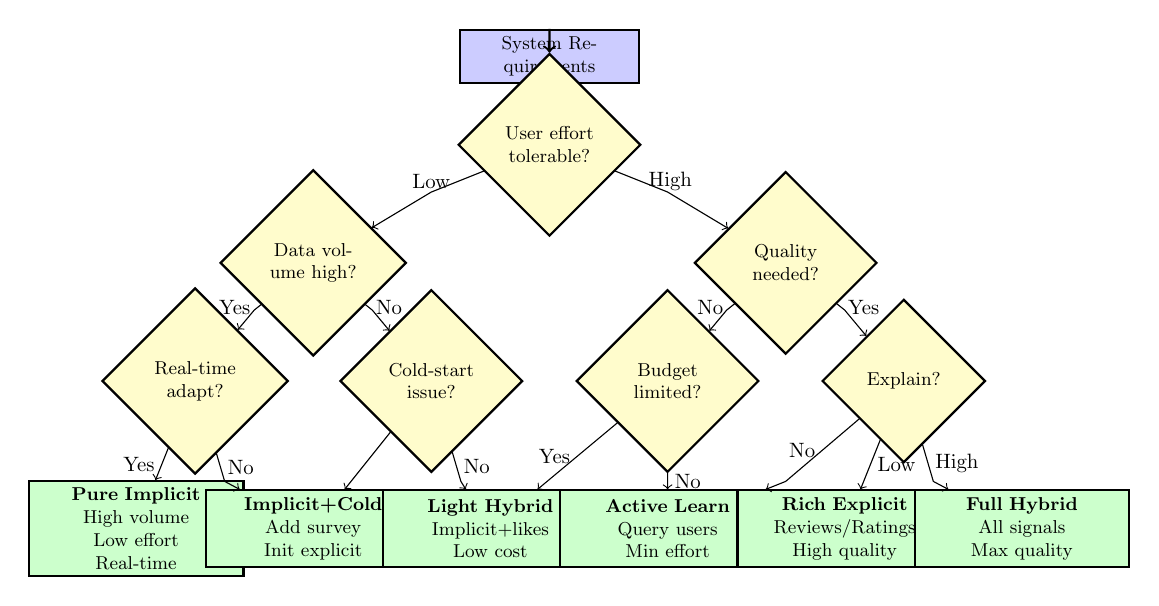
\begin{tikzpicture}[
    scale=0.75,
    transform shape,
    decision/.style={diamond, draw, thick, fill=yellow!20, text width=2.2cm, align=center, inner sep=2pt, font=\small},
    action/.style={rectangle, draw, thick, fill=blue!20, text width=2.8cm, align=center, minimum height=0.9cm, font=\small},
    result/.style={rectangle, draw, thick, fill=green!20, text width=3.4cm, align=center, minimum height=1.3cm, font=\small}
]

% Start
\node[action] (start) at (0,10) {System Requirements};

% First decision
\node[decision] (d1) at (0,8.5) {User effort tolerable?};

% Second level
\node[decision] (d2a) at (-4,6.5) {Data volume high?};
\node[decision] (d2b) at (4,6.5) {Quality needed?};

% Third level
\node[decision] (d3a) at (-6,4.5) {Real-time adapt?};
\node[decision] (d3b) at (-2,4.5) {Cold-start issue?};
\node[decision] (d3c) at (2,4.5) {Budget limited?};
\node[decision] (d3d) at (6,4.5) {Explain?};

% Results - IMPROVED TEXT FORMATTING
\node[result] (r1) at (-7,2) {\textbf{Pure Implicit}\\High volume\\Low effort\\Real-time};
\node[result] (r2) at (-4,2) {\textbf{Implicit+Cold}\\Add survey\\Init explicit};
\node[result] (r3) at (-1,2) {\textbf{Light Hybrid}\\Implicit+likes\\Low cost};
\node[result] (r4) at (2,2) {\textbf{Active Learn}\\Query users\\Min effort};
\node[result] (r5) at (5,2) {\textbf{Rich Explicit}\\Reviews/Ratings\\High quality};
\node[result] (r6) at (8,2) {\textbf{Full Hybrid}\\All signals\\Max quality};

% Arrows
\draw[thick, ->] (start) -- (d1);
\draw[->] (d1) -- node[left] {Low} (-2,7.7) -- (d2a);
\draw[->] (d1) -- node[right] {High} (2,7.7) -- (d2b);

\draw[->] (d2a) -- node[left] {Yes} (-5,5.7) -- (d3a);
\draw[->] (d2a) -- node[right] {No} (-3,5.7) -- (d3b);
\draw[->] (d2b) -- node[left] {No} (3,5.7) -- (d3c);
\draw[->] (d2b) -- node[right] {Yes} (5,5.7) -- (d3d);

\draw[->] (d3a) -- node[left] {Yes} (r1);
\draw[->] (d3a) -- node[right] {No} (-5.5,2.8) -- (r2);
\draw[->] (d3b) -- (r2);
\draw[->] (d3b) -- node[right] {No} (-1.5,2.8) -- (r3);
\draw[->] (d3c) -- node[left] {Yes} (r3);
\draw[->] (d3c) -- node[right] {No} (r4);
\draw[->] (d3d) -- node[left] {No} (4,2.8) -- (r4);
\draw[->] (d3d) -- node[right] {Low} (r5);
\draw[->] (d3d) -- node[right] {High} (6.5,2.8) -- (r6);

\end{tikzpicture}
\caption{Decision Flowchart for Feedback Strategy Selection}
\Description{A decision tree flowchart starting with system requirements and branching through decision nodes for user effort tolerance, data volume, real-time adaptation needs, cold-start issues, budget constraints, and explainability requirements. Each path leads to one of six recommended strategies: Pure Implicit, Implicit with Cold-start support, Lightweight Hybrid, Active Learning, Rich Explicit, or Full Hybrid approach.}
\label{fig:decision_flowchart}
\end{figure}

\textbf{Decision Framework Guidelines:}

\begin{enumerate}
    \item \textbf{User Effort Assessment}: 
    \begin{itemize}
        \item Low tolerance: Mobile apps, gaming, short sessions $\rightarrow$ Favor implicit
        \item High tolerance: Professional tools, high-value purchases $\rightarrow$ Consider explicit
    \end{itemize}
    
    \item \textbf{Data Volume Expectations}:
    \begin{itemize}
        \item High volume guaranteed: E-commerce, streaming $\rightarrow$ Implicit sufficient
        \item Limited interactions: Niche products, cold-start $\rightarrow$ Need explicit/hybrid
    \end{itemize}
    
    \item \textbf{Real-time Adaptation Requirements}:
    \begin{itemize}
        \item Essential: News, social feeds, live events $\rightarrow$ Implicit feedback
        \item Less critical: Periodic recommendations $\rightarrow$ Flexible on feedback type
    \end{itemize}
    
    \item \textbf{Quality vs. Cost Trade-offs}:
    \begin{itemize}
        \item Budget constrained: Implicit-only (no collection costs)
        \item Quality critical: Invest in hybrid with active learning
    \end{itemize}
    
    \item \textbf{Explainability Requirements}:
    \begin{itemize}
        \item High need: Healthcare, finance, education $\rightarrow$ Explicit + hybrid
        \item Low need: Entertainment, browsing $\rightarrow$ Implicit acceptable
    \end{itemize}
\end{enumerate}

\textbf{Implementation Checklist:}
\begin{itemize}
    \item[$\square$] Assess user base characteristics (tech-savvy, demographics, behavior patterns)
    \item[$\square$] Estimate expected interaction volume and frequency
    \item[$\square$] Define primary success metrics (accuracy, engagement, revenue, satisfaction)
    \item[$\square$] Evaluate budget for feedback collection and processing infrastructure
    \item[$\square$] Consider regulatory requirements (GDPR, CCPA, consent management)
    \item[$\square$] Plan for cold-start and new user scenarios
    \item[$\square$] Design bias detection and mitigation strategies
    \item[$\square$] Establish A/B testing framework for strategy validation
\end{itemize}

\subsection{Advanced Feedback Categorization}

\subsubsection{Feedback Granularity Spectrum}

\begin{figure}[!htbp]
\centering
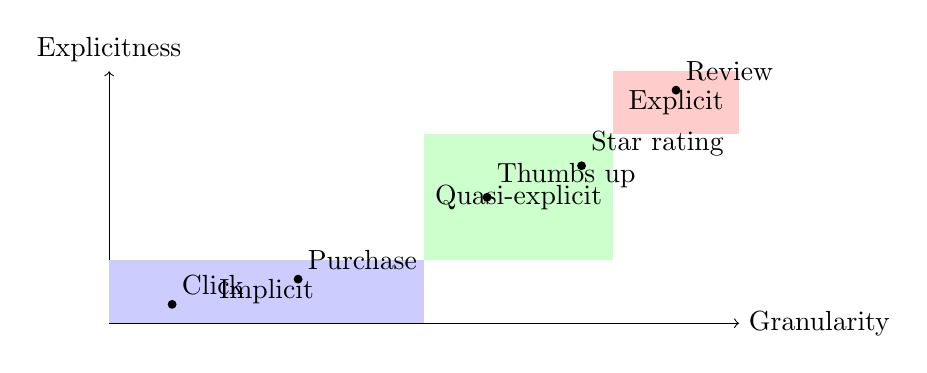
\begin{tikzpicture}[scale=0.8]
    \draw[->] (0,0) -- (10,0) node[right] {Granularity};
    \draw[->] (0,0) -- (0,4) node[above] {Explicitness};

    % Implicit region
    \fill[blue!20] (0,0) rectangle (5,1);
    \node at (2.5,0.5) {Implicit};

    % Quasi-explicit region
    \fill[green!20] (5,1) rectangle (8,3);
    \node at (6.5,2) {Quasi-explicit};

    % Explicit region
    \fill[red!20] (8,3) rectangle (10,4);
    \node at (9,3.5) {Explicit};

    % Example points
    \fill[black] (1,0.3) circle (2pt) node[above right] {Click};
    \fill[black] (3,0.7) circle (2pt) node[above right] {Purchase};
    \fill[black] (6,2) circle (2pt) node[above right] {Thumbs up};
    \fill[black] (7.5,2.5) circle (2pt) node[above right] {Star rating};
    \fill[black] (9,3.7) circle (2pt) node[above right] {Review};
\end{tikzpicture}
\caption{Feedback Granularity Spectrum}
\Description{A two-dimensional plot showing the feedback granularity spectrum with Granularity on the x-axis and Explicitness on the y-axis. The plot is divided into three colored regions: Implicit (blue, low explicitness), Quasi-explicit (green, medium), and Explicit (red, high). Example feedback types are plotted as points: Click (low), Purchase (low-medium), Thumbs up (medium), Star rating (medium-high), and Review (high).}
\label{fig:granularity_spectrum}
\end{figure}

\subsubsection{Multimodal Feedback Integration}

Modern systems increasingly combine multiple feedback modalities:
\begin{itemize}
    \item \textbf{Text-visual feedback}: Product images with review text
    \item \textbf{Audio-temporal feedback}: Music listening with skip behaviors
    \item \textbf{Spatial-temporal feedback}: Location-based preferences over time
    \item \textbf{Social-contextual feedback}: Group preferences in social settings
\end{itemize}

\subsubsection{Feedback Reliability Metrics}

Different feedback types have varying reliability characteristics:
\begin{itemize}
    \item \textbf{Internal consistency}: How consistent feedback is within a user
    \item \textbf{External validity}: How well feedback predicts actual behavior
    \item \textbf{Temporal stability}: How consistent feedback is over time
    \item \textbf{Cross-platform consistency}: Feedback agreement across different contexts
\end{itemize}

\subsection{Data Collection Mechanisms and Infrastructure}

\subsubsection{Implicit Feedback Collection}

Implicit feedback collection requires sophisticated tracking infrastructure:
\begin{itemize}
    \item \textbf{Event logging systems}: Real-time capture of user interactions
    \item \textbf{Cookie and session tracking}: Maintaining user identity across sessions
    \item \textbf{Device fingerprinting}: Cross-device user identification
    \item \textbf{Third-party data integration}: Incorporating external behavioral signals
\end{itemize}

\subsubsection{Explicit Feedback Collection}

Explicit feedback requires user interface design and motivation strategies:
\begin{itemize}
    \item \textbf{Rating interfaces}: Intuitive widgets for preference expression
    \item \textbf{Incentive systems}: Gamification and rewards for feedback provision
    \item \textbf{Progressive disclosure}: Multi-step feedback collection to reduce burden
    \item \textbf{Conversational interfaces}: Natural language feedback elicitation
\end{itemize}

\subsubsection{Hybrid Collection Strategies}

Combining collection approaches for comprehensive feedback:
\begin{itemize}
    \item \textbf{Implicit-explicit cascades}: Using implicit signals to trigger explicit feedback requests
    \item \textbf{Multi-touch attribution}: Combining multiple feedback sources for robust signals
    \item \textbf{Adaptive collection}: Dynamically adjusting feedback requests based on user engagement
\end{itemize}

\subsection{Privacy and Ethical Considerations}

\subsubsection{Privacy Implications by Feedback Type}

\begin{table}[h]
\centering
\caption{Privacy and Ethical Dimensions of Feedback Types}
\label{tab:privacy_ethics}
\begin{tabular}{@{}lccc@{}}
\toprule
Dimension & Implicit Feedback & Explicit Feedback & Key Concerns \\
\midrule
Data Sensitivity & Moderate & High & Personal opinion disclosure \\
Collection Transparency & Low & High & User awareness \\
Consent Requirements & Minimal & Explicit & Legal compliance \\
Anonymization Needs & Moderate & High & Identity protection \\
Behavioral Surveillance & High & Low & Privacy erosion \\
Data Minimization & Challenging & Feasible & Storage efficiency \\
User Control & Limited & High & Autonomy preservation \\
Third-party Sharing & Common & Rare & Data brokerage risks \\
\bottomrule
\end{tabular}
\end{table}

\subsubsection{Ethical Challenges}

Feedback collection raises several ethical concerns:
\begin{itemize}
    \item \textbf{Consent and transparency}: Users often unaware of implicit data collection
    \item \textbf{Algorithmic bias amplification}: Feedback patterns reflecting societal biases
    \item \textbf{Manipulation risks}: Systems influencing user behavior through feedback incentives
    \item \textbf{Privacy-utility trade-offs}: Balancing personalization benefits with privacy costs
\end{itemize}

\subsection{Visual Taxonomy and Conceptual Framework}

Figure~\ref{fig:comprehensive_taxonomy} presents our comprehensive taxonomy of feedback types.

\begin{figure}[!htbp]
\centering
\fbox{
\begin{minipage}{0.9\textwidth}
\textbf{Comprehensive Feedback Taxonomy}

\textbf{Main Categories:}
\begin{itemize}
\item \textbf{Implicit Feedback:} User behaviors without conscious effort
  \begin{itemize}
  \item \textit{Micro-level:} Clicks, dwell times, scrolls, hovers
  \item \textit{Meso-level:} Sessions, browsing patterns, purchase sequences
  \item \textit{Macro-level:} Longitudinal behavior, seasonal patterns, life-stage changes
  \end{itemize}
\item \textbf{Explicit Feedback:} Conscious user expressions
  \begin{itemize}
  \item \textit{Quantitative:} Ratings (1-5 stars), numerical scores, Likert scales
  \item \textit{Qualitative:} Reviews, comments, textual descriptions, tags
  \item \textit{Interactive:} Conversations, preference dialogs, custom profiles
  \end{itemize}
\item \textbf{Hybrid Approaches:} Combined implicit and explicit signals
  \begin{itemize}
  \item Multi-modal fusion, confidence-weighted integration, adaptive balancing
  \end{itemize}
\end{itemize}

\textbf{Key Properties by Category:}
\begin{tabular}{@{}lccc@{}}
\toprule
Property & Implicit & Explicit & Hybrid \\
\midrule
Data Abundance & Very High & Low & High \\
Noise Level & High & Low & Medium \\
User Effort & None & High & Medium \\
Temporal Resolution & Real-time & Delayed & Adaptive \\
Interpretability & Low & High & Medium \\
Scalability & High & Moderate & High \\
Privacy Sensitivity & High & Medium & Medium \\
Bias Susceptibility & Behavioral & Selection & Balanced \\
\bottomrule
\end{tabular}
\end{minipage}
}
\caption{Comprehensive taxonomy of implicit and explicit feedback types with hierarchical organization and key properties.}
\Description{A detailed hierarchical taxonomy table organizing feedback types into implicit and explicit categories. The implicit category includes behavioral signals (clicks, views, dwell time, scroll depth, search queries), engagement metrics (likes, shares, saves, follows, subscriptions), purchase indicators (add-to-cart, purchases, returns), and contextual signals (location, time, device, session length). The explicit category covers numeric ratings (star ratings, thumbs up/down, sliders, numerical scores), textual feedback (reviews, comments, tags, natural language), comparative feedback (rankings, pairwise comparisons, A/B preferences), and structured responses (surveys, questionnaires, feature ratings). Each type lists its characteristics including volume, reliability, cost, and noise level.}
\label{fig:comprehensive_taxonomy}
\end{figure}

\subsection{Domain-Specific Feedback Characteristics}

Different application domains exhibit unique feedback patterns and requirements:

\subsubsection{E-commerce Feedback Patterns}
\begin{itemize}
    \item High implicit feedback volume from browsing and purchasing
    \item Explicit reviews crucial for trust and explainability
    \item Strong correlation between implicit browsing and explicit purchasing decisions
\end{itemize}

\subsubsection{Entertainment Feedback Dynamics}
\begin{itemize}
    \item Implicit consumption patterns (watch time, skip rates) dominate
    \item Explicit ratings often retrospective and mood-dependent
    \item Social feedback (shares, recommendations) amplifies reach
\end{itemize}

\subsubsection{Social Media Feedback Ecology}
\begin{itemize}
    \item Implicit engagement metrics drive algorithmic ranking
    \item Explicit feedback sparse but highly influential
    \item Network effects create complex feedback cascades
\end{itemize}

This comprehensive taxonomy provides a foundation for understanding the rich landscape of feedback types in recommender systems, enabling more nuanced algorithm design and evaluation approaches.

\subsection{Modeling Approaches}
\label{subsec:modeling}

This section provides an extensive review of how implicit and explicit feedback are modeled across classical and modern approaches, including hybrid methods that integrate both types. We cover algorithmic foundations, mathematical formulations, and practical implementation considerations.

\subsection{Classical Approaches}

\subsubsection{Matrix Factorization Fundamentals}

Matrix factorization decomposes user-item interaction matrices into latent factor representations. For explicit feedback, the problem is formulated as:

\begin{equation}
\min_{P,Q} \sum_{(u,i) \in \mathcal{R}} (r_{ui} - p_u^T q_i)^2 + \lambda (\|P\|^2 + \|Q\|^2)
\label{eq:explicit_mf}
\end{equation}

where $r_{ui}$ represents explicit ratings, $p_u$ and $q_i$ are user and item latent factors, and $\lambda$ is a regularization parameter.

For implicit feedback, the formulation changes to handle binary preferences:

\begin{equation}
\min_{P,Q} \sum_{(u,i) \in \mathcal{R}^+} w_{ui} (1 - p_u^T q_i)^2 + \lambda (\|P\|^2 + \|Q\|^2)
\label{eq:implicit_mf}
\end{equation}

where $\mathcal{R}^+$ denotes observed implicit interactions and $w_{ui}$ represents confidence weights.

\subsubsection{Weighted Matrix Factorization (WMF)}

WMF addresses implicit feedback sparsity by treating unobserved interactions as negative signals with varying confidence:

\begin{equation}
\min_{P,Q} \sum_{u,i} c_{ui} (p_{ui} - p_u^T q_i)^2 + \lambda (\|P\|^2 + \|Q\|^2)
\label{eq:wmf}
\end{equation}

where $c_{ui} = \alpha r_{ui}$ for observed interactions and $c_{ui} = 1$ for unobserved ones, with $r_{ui}$ being the implicit feedback strength.

\subsubsection{Bayesian Personalized Ranking (BPR)}

BPR optimizes for ranking rather than rating prediction, using pairwise preferences:

\begin{equation}
\min_{\Theta} -\sum_{(u,i,j) \in D} \ln \sigma(\hat{r}_{ui} - \hat{r}_{uj}) + \lambda_\Theta \|\Theta\|^2
\label{eq:bpr}
\end{equation}

where $D$ contains triples $(u,i,j)$ indicating user $u$ prefers item $i$ over item $j$.

\subsection{Deep Learning Architectures}

\subsubsection{Neural Collaborative Filtering (NCF)}

NCF extends matrix factorization with neural networks:

\begin{equation}
\hat{y}_{ui} = f(p_u, q_i, p_u \odot q_i | \Theta)
\label{eq:ncf}
\end{equation}

where $f(\cdot)$ is a neural network that learns complex interaction patterns from both implicit and explicit feedback.

\subsubsection{Autoencoders for Implicit Feedback}

Denoising autoencoders reconstruct user feedback vectors:

\begin{equation}
\hat{r}_u = f_\theta(f_\phi(r_u + \epsilon))
\label{eq:autoencoder}
\end{equation}

where $\epsilon$ represents noise injection to improve generalization.

\subsubsection{Graph Neural Networks (GNNs)}

GNNs model user-item interactions as graphs:

\begin{equation}
h_u^{(l+1)} = \sigma\left(\sum_{v \in \mathcal{N}(u)} \frac{1}{\sqrt{|\mathcal{N}(u)||\mathcal{N}(v)|}} W^{(l)} h_v^{(l)}\right)
\label{eq:gnn}
\end{equation}

where $\mathcal{N}(u)$ denotes neighbors in the user-item interaction graph.

\subsection{Reinforcement Learning Approaches}

\subsubsection{Markov Decision Processes for Recommendations}

Recommendations are framed as sequential decision-making:

\begin{equation}
\pi^*(s) = \arg\max_\pi \mathbb{E}\left[\sum_{t=0}^\infty \gamma^t r(s_t, a_t) \bigg| s_0 = s, \pi\right]
\label{eq:rl_mdp}
\end{equation}

where states $s$ include user context, actions $a$ are item recommendations, and rewards $r$ come from implicit feedback.

\subsubsection{Contextual Bandits}

Multi-armed bandit approaches balance exploration and exploitation:

\begin{equation}
\mu_{t+1} = \mu_t + \alpha_t (r_t - \mu_t)
\label{eq:bandit_update}
\end{equation}

where $\mu_t$ tracks expected rewards from implicit user responses.

\subsection{Contrastive Learning Paradigms}

\subsubsection{SimCLR for Recommendations}

Contrastive learning maximizes agreement between different views of user-item interactions:

\begin{equation}
\mathcal{L} = -\log \frac{\exp(\text{sim}(z_i, z_j)/\tau)}{\sum_{k=1}^{2N} \mathbb{I}_{[k \neq i]} \exp(\text{sim}(z_i, z_k)/\tau)}
\label{eq:contrastive}
\end{equation}

where $z_i, z_j$ are representations from positive pairs and $\tau$ is temperature.

\subsubsection{Hybrid Contrastive Objectives}

Combining supervised and self-supervised learning:

\begin{equation}
\mathcal{L}_{hybrid} = \mathcal{L}_{supervised} + \lambda \mathcal{L}_{contrastive}
\label{eq:hybrid_contrastive}
\end{equation}

balancing explicit supervision with implicit structure learning.

\subsection{Modern Approaches}

\subsubsection{Deep Learning Models}
Neural networks have revolutionized RS modeling. Autoencoders handle implicit feedback sparsity through reconstruction \cite{sedhain2015autorec}. Convolutional Neural Networks (CNNs) process sequential behaviors \cite{tang2018personalized}. Graph Neural Networks (GNNs) model user-item interactions as graphs \cite{wang2019neural}.

\subsubsection{Reinforcement Learning}
Reinforcement Learning (RL) frames recommendations as sequential decision-making. Implicit feedback serves as rewards, with exploration-exploitation trade-offs \cite{zhao2018recommendations}. Explicit feedback can provide more precise reward signals \cite{chen2019large}.

\subsubsection{Contrastive Learning}
Self-supervised contrastive learning leverages implicit feedback for representation learning. Methods like SimCLR adapt to RS by contrasting user-item interactions \cite{wu2021self}. Hybrid approaches combine contrastive objectives with explicit supervision \cite{xie2022contrastive}.

\subsection{Implicit-to-Explicit Conversions}

Several techniques convert implicit feedback to pseudo-explicit ratings:
\begin{itemize}
    \item \textbf{Ordinal regression}: Maps implicit signals to rating scales \cite{weston2011wsabie}.
    \item \textbf{Confidence weighting}: Assigns confidence scores to implicit preferences \cite{he2016fast}.
    \item \textbf{Generative models}: Uses GANs to synthesize explicit feedback from implicit data \cite{wang2017irgan}.
\end{itemize}

\subsection{Hybrid Models}

Hybrid approaches jointly model both feedback types:
\begin{itemize}
    \item \textbf{Multi-task learning}: Optimizes separate objectives for implicit and explicit feedback \cite{ma2011learning}.
    \item \textbf{Unified frameworks}: Integrates feedback types in shared latent spaces \cite{lian2017cccfnet}.
    \item \textbf{Attention mechanisms}: Weights different feedback sources dynamically \cite{chen2017attentive}.
\end{itemize}

\subsection{Detailed Modeling Techniques}

\subsubsection{Neural Matrix Factorization}

Neural extensions of matrix factorization use multi-layer perceptrons to model non-linear interactions. For implicit feedback, models like NeuMF \cite{he2017neural} learn from binary preferences, achieving state-of-the-art performance on ranking tasks.

\subsubsection{Sequence Modeling}

Recurrent Neural Networks (RNNs) and Transformers capture temporal dependencies in implicit feedback sequences. Models like BERT4Rec \cite{sun2019bert4rec} treat recommendation as a sequence prediction problem.

\subsubsection{Graph-Based Approaches}

Graph Neural Networks model user-item interactions as heterogeneous graphs. Methods like LightGCN \cite{he2020lightgcn} propagate preferences through graph convolutions, effectively handling implicit feedback sparsity.

\subsubsection{Generative Models}

Variational Autoencoders (VAEs) and Generative Adversarial Networks (GANs) generate synthetic feedback. For implicit data, VAEs learn latent representations that reconstruct user behavior patterns.

\subsection{Hybrid Integration Strategies}

\subsubsection{Attention-Based Fusion}

Attention mechanisms dynamically weight feedback sources. For example, in a music recommender, recent explicit ratings might receive higher attention than older implicit plays.

\subsubsection{Multi-Modal Learning}

Combining feedback with content features (e.g., item descriptions) enhances modeling. Vision-language models process explicit reviews alongside implicit clicks.

\subsubsection{Cross-Feedback Translation}

Techniques translate between feedback types. For instance, using LLMs to generate explicit ratings from implicit patterns.

\subsection{Computational Complexity and Scalability}

Implicit feedback models must handle large-scale data. Techniques like negative sampling and distributed training enable scalability. Explicit feedback models are computationally lighter but data-scarce.

\subsection{Evaluation of Modeling Approaches}

Empirical studies show that hybrid models outperform single-type approaches. However, performance gains depend on domain and data quality.

\subsection{Case Studies}

\subsubsection{YouTube Recommendations}

YouTube uses implicit watch time extensively, combined with explicit likes/dislikes. Their system employs deep neural networks for real-time personalization.

\subsubsection{Amazon Product Recommendations}

Amazon integrates purchase history (implicit) with reviews (explicit) using collaborative filtering and content-based methods.

\subsection{Advanced Implementation Considerations}

\subsubsection{Hyperparameter Optimization Strategies}

Effective hyperparameter tuning is crucial for model performance:

\begin{itemize}
    \item \textbf{Grid Search vs. Random Search}: Random search often more efficient for high-dimensional spaces
    \item \textbf{Bayesian Optimization}: Gaussian processes for sample-efficient optimization
    \item \textbf{AutoML Approaches}: Automated machine learning for hyperparameter discovery
    \item \textbf{Domain-Specific Tuning}: Different optimal parameters for implicit vs. explicit feedback
\end{itemize}

\subsubsection{Model Interpretability and Explainability}

Understanding model decisions is increasingly important:

\begin{itemize}
    \item \textbf{Attention Visualization}: Interpreting which feedback sources influence predictions
    \item \textbf{Feature Importance}: Identifying key implicit signals and explicit features
    \item \textbf{Counterfactual Explanations}: Explaining recommendations through "what-if" scenarios
    \item \textbf{User-Centric Explanations}: Translating technical model outputs to user-understandable insights
\end{itemize}

\subsubsection{Online Learning and Adaptation}

Systems must adapt to evolving user preferences:

\begin{itemize}
    \item \textbf{Incremental Learning}: Updating models with new feedback without full retraining
    \item \textbf{Concept Drift Detection}: Identifying when user preferences change significantly
    \item \textbf{Temporal Regularization}: Balancing historical and recent feedback appropriately
    \item \textbf{Context-Aware Updates}: Adapting to changing situational contexts
\end{itemize}

\subsubsection{Computational Resource Management}

Efficient deployment requires careful resource allocation:

\begin{itemize}
    \item \textbf{Model Compression}: Reducing model size for edge deployment
    \item \textbf{Inference Optimization}: Fast prediction serving for real-time recommendations
    \item \textbf{Caching Strategies}: Intelligent caching of user representations and item embeddings
    \item \textbf{Distributed Serving}: Scaling recommendation serving across multiple machines
\end{itemize}

\subsection{Emerging Algorithmic Paradigms}

\subsubsection{Multimodal Recommender Systems}

Integrating multiple data modalities for richer recommendations:

\begin{itemize}
    \item \textbf{Vision-Language Models}: Processing product images with textual reviews
    \item \textbf{Audio-Textual Integration}: Combining music audio features with user listening history
    \item \textbf{Cross-Modal Translation}: Converting between different feedback modalities
    \item \textbf{Multimodal Fusion Architectures}: Attention-based fusion of heterogeneous signals
\end{itemize}

\subsubsection{Causal Inference in Recommendations}

Understanding causal relationships rather than mere correlations:

\begin{itemize}
    \item \textbf{Causal Graphs}: Modeling causal pathways from feedback to user satisfaction
    \item \textbf{Intervention Analysis}: Simulating the effects of different recommendation strategies
    \item \textbf{Counterfactual Reasoning}: Estimating what would have happened under different conditions
    \item \textbf{Bias Mitigation}: Removing spurious correlations through causal methods
\end{itemize}

\subsubsection{Federated and Privacy-Preserving Learning}

Collaborative learning without compromising privacy:

\begin{itemize}
    \item \textbf{Federated Matrix Factorization}: Distributed training across user devices
    \item \textbf{Differential Privacy}: Adding noise to protect individual feedback
    \item \textbf{Secure Multi-Party Computation}: Privacy-preserving collaborative filtering
    \item \textbf{Homomorphic Encryption}: Encrypted computation on sensitive feedback data
\end{itemize}

\subsubsection{Continual and Lifelong Learning}

Adapting to evolving user preferences over time:

\begin{itemize}
    \item \textbf{Catastrophic Forgetting Prevention}: Maintaining old knowledge while learning new patterns
    \item \textbf{Elastic Weight Consolidation}: Protecting important parameters during updates
    \item \textbf{Progressive Neural Networks}: Growing network capacity for new tasks
    \item \textbf{Memory Replay}: Rehearsing past experiences to maintain performance
\end{itemize}

\subsection{Open Challenges in Modeling}

\begin{itemize}
    \item Handling feedback conflicts (e.g., clicking but not purchasing).
    \item Modeling long-term vs. short-term preferences.
    \item Incorporating user context and demographics.
\end{itemize}


\section{Evaluation Frameworks and Bias Analysis}
\label{sec:evaluation}

This section presents comprehensive evaluation methodologies specifically designed for feedback-aware recommender systems. We address fundamental challenges in fair comparison across feedback types and present frameworks for bias detection and mitigation.

\begin{figure}[ht]
\centering
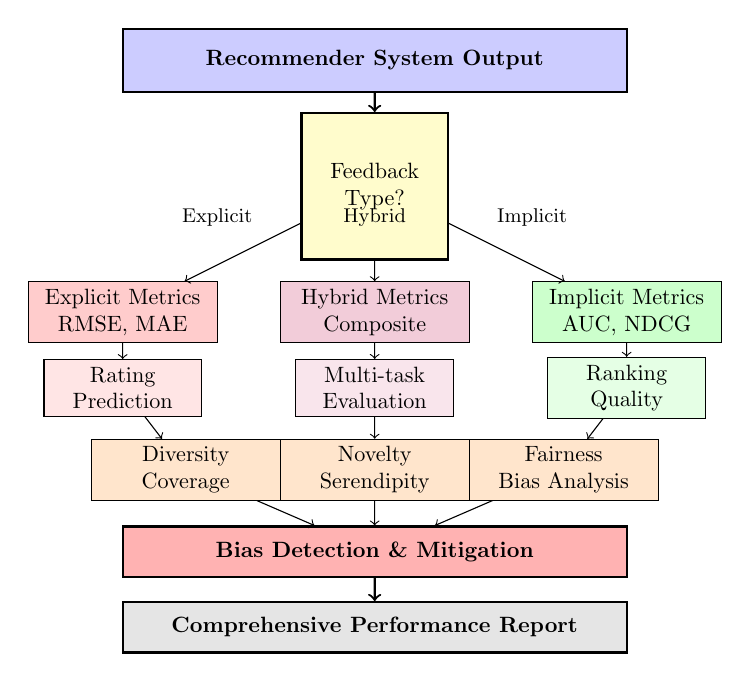
\begin{tikzpicture}[scale=0.8, transform shape]
    % Input layer
    \node[rectangle, draw, thick, fill=blue!20, minimum width=8cm, minimum height=1cm, align=center] (input) at (0,8) {\textbf{Recommender System Output}};
    
    % Decision diamond
    \node[regular polygon, regular polygon sides=4, draw, thick, fill=yellow!20, minimum width=2cm, minimum height=1.5cm, align=center] (decision) at (0,6) {Feedback\\Type?};
    
    % Explicit path
    \node[rectangle, draw, fill=red!20, minimum width=3cm, minimum height=0.8cm, align=center] (explicit_metrics) at (-4,4) {Explicit Metrics\\RMSE, MAE};
    \node[rectangle, draw, fill=red!10, minimum width=2.5cm, minimum height=0.6cm, align=center] (rating_pred) at (-4,2.8) {Rating\\Prediction};
    
    % Implicit path
    \node[rectangle, draw, fill=green!20, minimum width=3cm, minimum height=0.8cm, align=center] (implicit_metrics) at (4,4) {Implicit Metrics\\AUC, NDCG};
    \node[rectangle, draw, fill=green!10, minimum width=2.5cm, minimum height=0.6cm, align=center] (ranking) at (4,2.8) {Ranking\\Quality};
    
    % Hybrid path
    \node[rectangle, draw, fill=purple!20, minimum width=3cm, minimum height=0.8cm, align=center] (hybrid_metrics) at (0,4) {Hybrid Metrics\\Composite};
    \node[rectangle, draw, fill=purple!10, minimum width=2.5cm, minimum height=0.6cm, align=center] (multi_task) at (0,2.8) {Multi-task\\Evaluation};
    
    % Common evaluation dimensions
    \node[rectangle, draw, fill=orange!20, minimum width=3cm, minimum height=0.8cm, align=center] (diversity) at (-3,1.5) {Diversity\\Coverage};
    \node[rectangle, draw, fill=orange!20, minimum width=3cm, minimum height=0.8cm, align=center] (novelty) at (0,1.5) {Novelty\\Serendipity};
    \node[rectangle, draw, fill=orange!20, minimum width=3cm, minimum height=0.8cm, align=center] (fairness) at (3,1.5) {Fairness\\Bias Analysis};
    
    % Bias detection
    \node[rectangle, draw, thick, fill=red!30, minimum width=8cm, minimum height=0.8cm, align=center] (bias_detection) at (0,0.2) {\textbf{Bias Detection \& Mitigation}};
    
    % Final evaluation
    \node[rectangle, draw, thick, fill=gray!20, minimum width=8cm, minimum height=0.8cm, align=center] (final) at (0,-1) {\textbf{Comprehensive Performance Report}};
    
    % Arrows
    \draw[thick, ->] (input) -- (decision);
    \draw[->] (decision) -- (-2,5) -- (explicit_metrics);
    \draw[->] (decision) -- (hybrid_metrics);
    \draw[->] (decision) -- (2,5) -- (implicit_metrics);
    
    \draw[->] (explicit_metrics) -- (rating_pred);
    \draw[->] (implicit_metrics) -- (ranking);
    \draw[->] (hybrid_metrics) -- (multi_task);
    
    \draw[->] (rating_pred) -- (diversity);
    \draw[->] (multi_task) -- (novelty);
    \draw[->] (ranking) -- (fairness);
    
    \draw[->] (diversity) -- (bias_detection);
    \draw[->] (novelty) -- (bias_detection);
    \draw[->] (fairness) -- (bias_detection);
    
    \draw[thick, ->] (bias_detection) -- (final);
    
    % Labels
    \node[font=\small] at (-2.5,5.5) {Explicit};
    \node[font=\small] at (0,5.5) {Hybrid};
    \node[font=\small] at (2.5,5.5) {Implicit};
    
\end{tikzpicture}
\caption{Comprehensive Evaluation Framework for Feedback-Aware Recommender Systems}
\label{fig:evaluation_framework}
\end{figure}

Figure~\ref{fig:evaluation_framework} illustrates our systematic evaluation approach that adapts metrics and methodologies based on the underlying feedback mechanism while ensuring comprehensive assessment across multiple quality dimensions.

\subsection{Feedback-Specific Evaluation Challenges}

Traditional evaluation approaches often fail to account for the fundamental differences between implicit and explicit feedback, leading to biased comparisons and misleading conclusions about system performance.

\subsubsection{The Evaluation Gap Problem}
Current evaluation practices treat all recommender systems uniformly, regardless of their underlying feedback mechanisms. This creates several critical issues:

\textbf{Metric Appropriateness}: Metrics designed for explicit feedback (e.g., RMSE for rating prediction) may not adequately capture the effectiveness of implicit feedback systems optimized for ranking.

\textbf{Ground Truth Assumptions}: Implicit feedback systems lack clear negative examples, making standard precision/recall calculations problematic without careful consideration of negative sampling strategies.

\textbf{Temporal Considerations}: Implicit feedback often exhibits different temporal dynamics than explicit feedback, requiring evaluation protocols that account for these differences.

\subsection{Comprehensive Evaluation Framework}

We propose a multi-dimensional evaluation framework that accounts for feedback characteristics while enabling fair comparison across system types.

\subsubsection{Core Evaluation Dimensions}

\textbf{Dimension 1: Predictive Accuracy}
\begin{itemize}
    \item \textit{For Explicit Feedback}: RMSE, MAE for rating prediction
    \item \textit{For Implicit Feedback}: AUC, Hit Ratio, NDCG for ranking
    \item \textit{For Hybrid Systems}: Composite metrics combining both paradigms
\end{itemize}

\textbf{Dimension 2: Ranking Quality}
\begin{itemize}
    \item \textit{Precision@K}: $P@K = \frac{|R@K \cap T|}{K}$
    \item \textit{Recall@K}: $R@K = \frac{|R@K \cap T|}{|T|}$
    \item \textit{NDCG@K}: $NDCG@K = \frac{DCG@K}{IDCG@K}$
    \item \textit{Mean Reciprocal Rank}: $MRR = \frac{1}{|Q|}\sum_{i=1}^{|Q|}\frac{1}{rank_i}$
\end{itemize}

\textbf{Dimension 3: Diversity and Coverage}
\begin{itemize}
    \item \textit{Intra-list Diversity}: Average pairwise dissimilarity within recommendation lists
    \item \textit{Catalog Coverage}: Percentage of items recommended across all users
    \item \textit{User Coverage}: Percentage of users receiving satisfactory recommendations
\end{itemize}

\textbf{Dimension 4: Novelty and Serendipity}
\begin{itemize}
    \item \textit{Novelty}: Average popularity of recommended items (inversely related)
    \item \textit{Serendipity}: Unexpected but relevant recommendations
    \item \textit{Discovery Rate}: New items successfully introduced to users
\end{itemize}

\subsubsection{Feedback-Aware Evaluation Protocols}

\textbf{Protocol 1: Stratified Evaluation by Feedback Type}
\begin{algorithm}[h]
\caption{Feedback-Stratified Evaluation}
\begin{algorithmic}[1]
\STATE Input: Dataset $D$, Feedback types $F = \{f_1, f_2, ..., f_k\}$
\STATE Output: Performance metrics $M = \{m_1, m_2, ..., m_k\}$
\FOR{each feedback type $f_i \in F$}
    \STATE $D_i \leftarrow$ Extract data of type $f_i$ from $D$
    \STATE $Train_i, Test_i \leftarrow$ Split $D_i$ temporally
    \STATE $Model_i \leftarrow$ Train model on $Train_i$
    \STATE $Pred_i \leftarrow$ Generate predictions for $Test_i$
    \STATE $m_i \leftarrow$ Evaluate $Pred_i$ using appropriate metrics for $f_i$
\ENDFOR
\RETURN $M$
\end{algorithmic}
\end{algorithm}

\textbf{Protocol 2: Cross-Feedback Validation}
For hybrid systems, we evaluate performance when feedback types are available in different combinations:
\begin{itemize}
    \item \textit{Full Information}: All feedback types available
    \item \textit{Partial Information}: Subsets of feedback types
    \item \textit{Cold-Start}: No feedback available for new users/items
    \item \textit{Feedback Transition}: Performance when feedback types change over time
\end{itemize}

\subsection{Bias Detection and Analysis Framework}

Bias in recommender systems can significantly impact both system performance and user experience. We provide comprehensive analysis of bias types and detection methodologies.

\subsubsection{Taxonomy of Biases in Feedback-Based Systems}

\begin{figure}[ht]
\centering
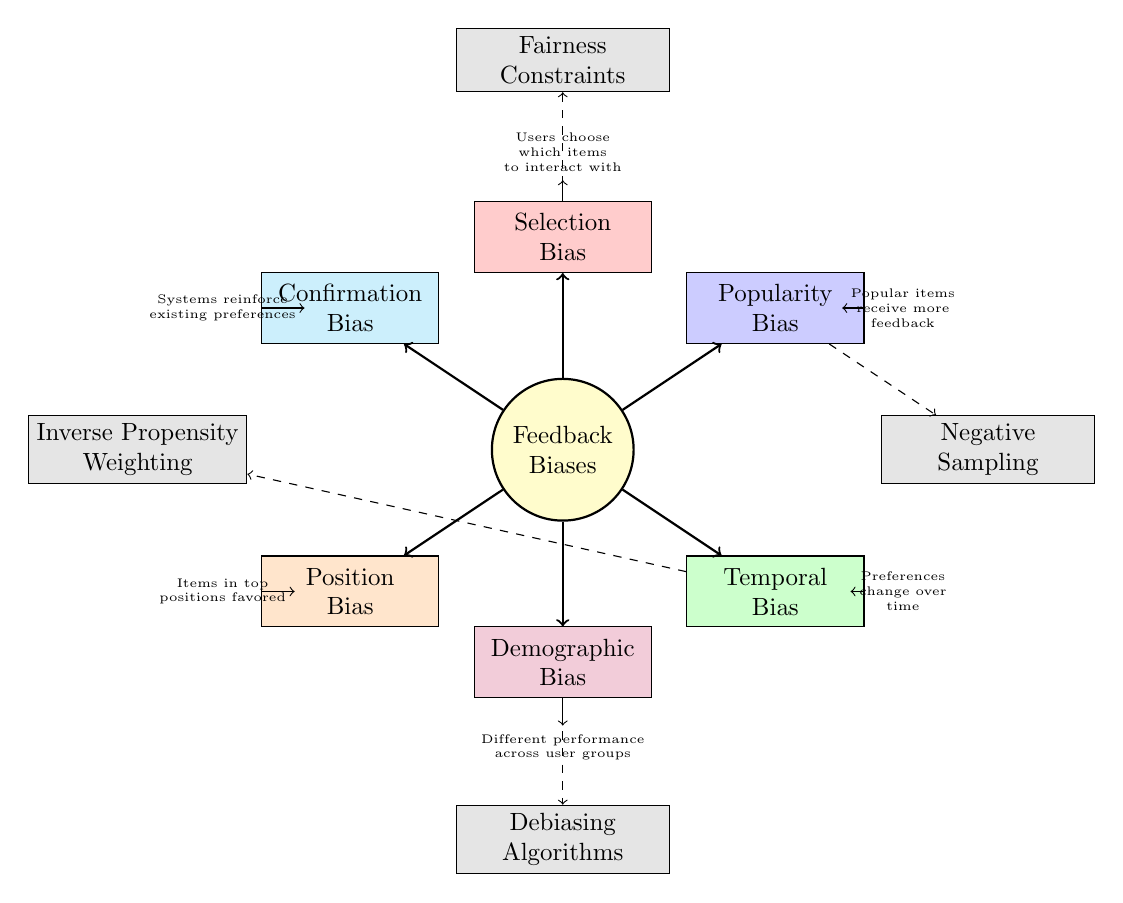
\begin{tikzpicture}[scale=0.9, transform shape]
    % Central node
    \node[circle, draw, thick, fill=yellow!20, minimum size=2cm, align=center] (center) at (0,0) {Feedback\\Biases};
    
    % Bias types around the circle
    \node[rectangle, draw, fill=red!20, minimum width=2.5cm, minimum height=1cm, align=center] (selection) at (0,3) {Selection\\Bias};
    \node[rectangle, draw, fill=blue!20, minimum width=2.5cm, minimum height=1cm, align=center] (popularity) at (3,2) {Popularity\\Bias};
    \node[rectangle, draw, fill=green!20, minimum width=2.5cm, minimum height=1cm, align=center] (temporal) at (3,-2) {Temporal\\Bias};
    \node[rectangle, draw, fill=purple!20, minimum width=2.5cm, minimum height=1cm, align=center] (demographic) at (0,-3) {Demographic\\Bias};
    \node[rectangle, draw, fill=orange!20, minimum width=2.5cm, minimum height=1cm, align=center] (position) at (-3,-2) {Position\\Bias};
    \node[rectangle, draw, fill=cyan!20, minimum width=2.5cm, minimum height=1cm, align=center] (confirmation) at (-3,2) {Confirmation\\Bias};
    
    % Impact descriptions
    \node[align=center, font=\tiny] (sel_desc) at (0,4.2) {Users choose\\which items\\to interact with};
    \node[align=center, font=\tiny] (pop_desc) at (4.8,2) {Popular items\\receive more\\feedback};
    \node[align=center, font=\tiny] (temp_desc) at (4.8,-2) {Preferences\\change over\\time};
    \node[align=center, font=\tiny] (demo_desc) at (0,-4.2) {Different performance\\across user groups};
    \node[align=center, font=\tiny] (pos_desc) at (-4.8,-2) {Items in top\\positions favored};
    \node[align=center, font=\tiny] (conf_desc) at (-4.8,2) {Systems reinforce\\existing preferences};
    
    % Mitigation strategies
    \node[rectangle, draw, fill=gray!20, minimum width=3cm, minimum height=0.7cm, align=center] (mit1) at (-6,0) {Inverse Propensity\\Weighting};
    \node[rectangle, draw, fill=gray!20, minimum width=3cm, minimum height=0.7cm, align=center] (mit2) at (6,0) {Negative\\Sampling};
    \node[rectangle, draw, fill=gray!20, minimum width=3cm, minimum height=0.7cm, align=center] (mit3) at (0,5.5) {Fairness\\Constraints};
    \node[rectangle, draw, fill=gray!20, minimum width=3cm, minimum height=0.7cm, align=center] (mit4) at (0,-5.5) {Debiasing\\Algorithms};
    
    % Arrows from center to bias types
    \draw[thick, ->] (center) -- (selection);
    \draw[thick, ->] (center) -- (popularity);
    \draw[thick, ->] (center) -- (temporal);
    \draw[thick, ->] (center) -- (demographic);
    \draw[thick, ->] (center) -- (position);
    \draw[thick, ->] (center) -- (confirmation);
    
    % Arrows to descriptions
    \draw[->] (selection) -- (sel_desc);
    \draw[->] (popularity) -- (pop_desc);
    \draw[->] (temporal) -- (temp_desc);
    \draw[->] (demographic) -- (demo_desc);
    \draw[->] (position) -- (pos_desc);
    \draw[->] (confirmation) -- (conf_desc);
    
    % Arrows to mitigation strategies
    \draw[dashed, ->] (selection) -- (mit3);
    \draw[dashed, ->] (popularity) -- (mit2);
    \draw[dashed, ->] (temporal) -- (mit1);
    \draw[dashed, ->] (demographic) -- (mit4);
    
\end{tikzpicture}
\caption{Comprehensive Bias Analysis Framework for Feedback-Aware Systems}
\label{fig:bias_analysis}
\end{figure}

Figure~\ref{fig:bias_analysis} illustrates the major sources of bias in feedback-based recommender systems and their corresponding mitigation strategies, emphasizing the need for systematic bias detection and correction across all feedback types.

\textbf{Selection Bias}
Users choose which items to interact with or rate, creating biased training data:
\begin{equation}
P(feedback|item) \neq P(feedback|item, selection)
\end{equation}

\textit{Detection}: Compare feedback distributions with random samples
\textit{Impact}: Underrepresentation of certain item types or user groups

\textbf{Popularity Bias}
Over-representation of popular items in both training data and recommendations:
\begin{equation}
Popularity\_Bias = \frac{\sum_{i \in R} popularity(i)}{|R|} - \frac{\sum_{i \in C} popularity(i)}{|C|}
\end{equation}
where $R$ is the recommendation set and $C$ is the catalog.

\textbf{Temporal Bias}
Changing preferences and item availability over time affecting evaluation:
\begin{equation}
Temporal\_Drift(t) = \frac{||P_t - P_{t-\Delta}||_2}{||P_{t-\Delta}||_2}
\end{equation}
where $P_t$ represents preference distribution at time $t$.

\textbf{Demographic Bias}
Differential performance across user demographics:
\begin{equation}
Fairness\_Gap = \max_{g_i, g_j \in G} |Performance(g_i) - Performance(g_j)|
\end{equation}
where $G$ is the set of demographic groups.

\subsubsection{Bias Mitigation Strategies}

\textbf{For Implicit Feedback Systems}:
\begin{itemize}
    \item \textit{Inverse Propensity Weighting}: Weight observations by inverse of selection probability
    \item \textit{Negative Sampling Strategies}: Carefully select negative examples to reduce bias
    \item \textit{Temporal Debiasing}: Account for time-varying preferences and item popularity
\end{itemize}

\textbf{For Explicit Feedback Systems}:
\begin{itemize}
    \item \textit{Rating Bias Correction}: Normalize for user rating tendencies and item popularity
    \item \textit{Missing Data Imputation}: Use principled approaches for handling missing ratings
    \item \textit{Cross-Validation Strategies}: Ensure representative train/test splits
\end{itemize}

\textbf{For Hybrid Systems}:
\begin{itemize}
    \item \textit{Multi-Objective Optimization}: Balance accuracy and fairness across feedback types
    \item \textit{Bias-Aware Fusion}: Weight feedback sources considering their bias characteristics
    \item \textit{Ensemble Debiasing}: Use diverse models to reduce systematic biases
\end{itemize}

\subsection{Experimental Design Considerations}

\subsubsection{Dataset Requirements and Characteristics}

\textbf{Essential Dataset Properties}:
\begin{itemize}
    \item \textit{Multi-Modal Feedback}: Datasets containing both implicit and explicit signals
    \item \textit{Temporal Information}: Timestamps enabling temporal analysis
    \item \textit{Rich Metadata}: User and item characteristics for bias analysis
    \item \textit{Sufficient Scale}: Adequate size for robust statistical analysis
\end{itemize}

\textbf{Benchmark Datasets for Feedback Research}:
\begin{table}[h]
\centering
\caption{Key Datasets for Feedback-Aware Evaluation}
\label{tab:datasets}
\begin{tabular}{@{}lcccc@{}}
\toprule
Dataset & Domain & Implicit & Explicit & Users/Items \\
\midrule
Amazon Product & E-commerce & \checkmark & \checkmark & 8M/2.3M \\
Netflix & Streaming & \checkmark & \checkmark & 480K/17K \\
Last.fm & Music & \checkmark & \checkmark & 360K/160K \\
Yelp & Reviews & \checkmark & \checkmark & 1.6M/200K \\
MovieLens-25M & Movies & \checkmark & \checkmark & 280K/58K \\
\bottomrule
\end{tabular}
\end{table}

\subsubsection{Statistical Testing and Significance}

\textbf{Appropriate Statistical Tests}:
\begin{itemize}
    \item \textit{Wilcoxon Signed-Rank Test}: For non-parametric paired comparisons
    \item \textit{McNemar's Test}: For comparing binary classification performance
    \item \textit{Bootstrap Confidence Intervals}: For robust uncertainty estimation
    \item \textit{Multiple Comparison Correction}: Bonferroni or FDR correction for multiple metrics
\end{itemize}

\textbf{Effect Size Measures}:
Beyond statistical significance, we emphasize practical significance:
\begin{equation}
Cohen's\_d = \frac{\mu_1 - \mu_2}{\sqrt{\frac{\sigma_1^2 + \sigma_2^2}{2}}}
\end{equation}

\subsection{Advanced Evaluation Methodologies}

\subsubsection{Counterfactual Evaluation}
For scenarios where online A/B testing is impractical:

\textbf{Inverse Propensity Scoring (IPS)}:
\begin{equation}
\hat{R}_{IPS} = \frac{1}{n}\sum_{i=1}^n \frac{r_i \cdot \mathbf{1}[a_i = \pi(x_i)]}{p(a_i|x_i)}
\end{equation}
where $r_i$ is the reward, $a_i$ is the action, $\pi(x_i)$ is the policy, and $p(a_i|x_i)$ is the propensity score.

\textbf{Doubly Robust Estimation}:
Combines direct method and IPS for more robust evaluation:
\begin{equation}
\hat{R}_{DR} = \hat{R}_{DM} + \frac{1}{n}\sum_{i=1}^n \frac{\mathbf{1}[a_i = \pi(x_i)]}{p(a_i|x_i)}(r_i - \hat{r}(x_i, a_i))
\end{equation}

\subsubsection{Multi-Stakeholder Evaluation}
Modern recommender systems must balance multiple stakeholder interests:

\textbf{User Satisfaction Metrics}:
\begin{itemize}
    \item \textit{Click-Through Rate}: Immediate engagement
    \item \textit{Dwell Time}: Content consumption depth
    \item \textit{Return Rate}: Long-term user retention
    \item \textit{Explicit Satisfaction}: Direct user feedback on recommendations
\end{itemize}

\textbf{Platform Metrics}:
\begin{itemize}
    \item \textit{Catalog Turnover}: Rate of new item discovery
    \item \textit{Revenue Impact}: Business value of recommendations
    \item \textit{Computational Efficiency}: Resource utilization
\end{itemize}

\textbf{Creator/Provider Metrics}:
\begin{itemize}
    \item \textit{Exposure Fairness}: Equal opportunity for item visibility
    \item \textit{Long-tail Coverage}: Support for niche content
    \item \textit{Creator Diversity}: Representation across different providers
\end{itemize}

\subsection{Reproducibility and Standardization}

\subsubsection{Evaluation Framework Implementation}
To promote reproducible research, we provide:

\begin{itemize}
    \item \textbf{Standardized Metrics}: Reference implementations of feedback-aware metrics
    \item \textbf{Evaluation Protocols}: Step-by-step procedures for different scenarios
    \item \textbf{Bias Detection Tools}: Automated analysis of common bias types
    \item \textbf{Statistical Testing Suite}: Appropriate tests for different comparison scenarios
\end{itemize}

\subsubsection{Best Practices for Reporting Results}

\textbf{Essential Reporting Elements}:
\begin{itemize}
    \item \textit{Dataset Characteristics}: Detailed description of feedback types and distributions
    \item \textit{Evaluation Protocol}: Clear specification of train/test procedures
    \item \textit{Statistical Testing}: Significance tests and confidence intervals
    \item \textit{Bias Analysis}: Assessment of potential biases and mitigation strategies
    \item \textit{Computational Requirements}: Resource usage and scalability considerations
\end{itemize}

This comprehensive evaluation framework enables fair comparison of recommender systems across different feedback types while accounting for their inherent characteristics and potential biases. By adopting these methodologies, the research community can make more reliable progress in developing effective feedback-aware recommendation systems.

\begin{itemize}
    \item \textbf{Implicit feedback} often uses binary relevance (clicked/not clicked), favoring ranking accuracy over absolute preference strength.
    \item \textbf{Explicit feedback} incorporates preference strength, allowing for more nuanced evaluation of recommendation quality.
    \item \textbf{Hybrid approaches} require careful calibration to balance ranking and rating prediction objectives.
\end{itemize}

The mathematical formulations reveal important differences:

\begin{equation}
\text{Precision@K} = \frac{|\{i \in \text{top-K} \cap \text{relevant}\}|}{K}
\label{eq:precision_k}
\end{equation}

\begin{equation}
\text{NDCG@K} = \frac{1}{|U|} \sum_{u \in U} \frac{\sum_{i=1}^K \frac{rel_{u,i}}{log_2(i+1)}}{\sum_{i=1}^{|REL_u|} \frac{1}{log_2(i+1)}}
\label{eq:ndcg_k}
\end{equation}

where $rel_{u,i}$ represents relevance scores that differ significantly between implicit (binary) and explicit (graded) feedback.

\subsubsection{Rating Prediction Metrics}
Root Mean Square Error (RMSE) and Mean Absolute Error (MAE) evaluate explicit rating predictions:

\begin{equation}
\text{RMSE} = \sqrt{\frac{1}{|R|} \sum_{(u,i) \in R} (\hat{r}_{ui} - r_{ui})^2}
\label{eq:rmse}
\end{equation}

\begin{equation}
\text{MAE} = \frac{1}{|R|} \sum_{(u,i) \in R} |\hat{r}_{ui} - r_{ui}|
\label{eq:mae}
\end{equation}

These metrics are less applicable to implicit feedback, which lacks ground-truth ratings, necessitating alternative evaluation approaches.

\subsubsection{Area Under the Curve (AUC) Metrics}
For implicit feedback evaluation, AUC-based metrics provide robust ranking assessment:

\begin{equation}
\text{AUC} = \frac{1}{|U|} \sum_{u \in U} \frac{1}{|I_u^+||I_u^-|} \sum_{i^+ \in I_u^+} \sum_{i^- \in I_u^-} \mathbb{I}(\hat{r}_{ui^+} > \hat{r}_{ui^-})
\label{eq:auc}
\end{equation}

where $I_u^+$ and $I_u^-$ represent positive and negative feedback items for user $u$.

\subsection{Evaluation Biases and Challenges}

\subsubsection{Dataset Biases}
Public datasets exhibit various biases that affect evaluation reliability:

\begin{table}[h]
\centering
\caption{Evaluation Biases in Different Feedback Types}
\label{tab:evaluation_biases}
\begin{tabular}{@{}lccc@{}}
\toprule
Bias Type & Implicit Feedback & Explicit Feedback & Mitigation Strategies \\
\midrule
Popularity Bias & High (rich-get-richer) & Moderate & Inverse propensity scoring \\
Position Bias & Very High & Moderate & Position debiasing, randomization \\
Selection Bias & Low & Very High & Inverse propensity weighting \\
Confirmation Bias & Moderate & High & Counterfactual evaluation \\
Temporal Bias & High & Moderate & Time-aware validation \\
Demographic Bias & Moderate & High & Fairness-aware evaluation \\
\bottomrule
\end{tabular}
\end{table}

\subsubsection{User Behavior Interpretations}
Implicit feedback interpretations can be misleading:

\begin{itemize}
    \item \textbf{Engagement vs. Interest}: Long watch times may indicate engagement or involuntary attention (e.g., background TV)
    \item \textbf{Contextual Influences}: Clicks may result from curiosity, social pressure, or algorithmic manipulation
    \item \textbf{Behavioral Variability}: User interaction patterns vary significantly across demographics and contexts
    \item \textbf{False Negatives}: Lack of interaction doesn't necessarily indicate lack of interest
\end{itemize}

Explicit feedback, while clearer, has its own interpretation challenges:

\begin{itemize}
    \item \textbf{Mood-Dependent Ratings}: Emotional state influences rating consistency
    \item \textbf{Social Desirability Bias}: Users provide socially acceptable rather than genuine opinions
    \item \textbf{Scale Interpretation Variance}: Different users interpret rating scales differently
    \item \textbf{Recency Effects}: Recent experiences disproportionately influence feedback
\end{itemize}

\subsection{Advanced Evaluation Frameworks}

\subsubsection{Novelty and Diversity Metrics}

Beyond accuracy, diversity and novelty are crucial for user satisfaction:

\begin{equation}
\text{Novelty} = -\log_2(\text{popularity}(i))
\label{eq:novelty}
\end{equation}

\begin{equation}
\text{Diversity} = 1 - \frac{\sum_{i,j \in L} s(i,j)}{|L|(|L|-1)}
\label{eq:diversity}
\end{equation}

where $s(i,j)$ measures similarity between recommended items and $L$ is the recommendation list.

\subsubsection{Serendipity Metrics}

Measuring unexpected relevant recommendations:

\begin{equation}
\text{Serendipity} = \frac{1}{|U|} \sum_u \frac{|\{i \in L_u | rel(u,i) \land unexpected(u,i)\}|}{|L_u|}
\label{eq:serendipity}
\end{equation}

\subsubsection{Coverage Metrics}

Assessing catalog utilization:

\begin{equation}
\text{Catalog Coverage} = \frac{|\bigcup_u L_u|}{|\mathcal{I}|}
\label{eq:coverage}
\end{equation}

\begin{equation}
\text{User Coverage} = \frac{|\{u | |L_u| > 0\}|}{|U|}
\label{eq:user_coverage}
\end{equation}

\subsection{User-Centric Evaluation Methods}

\subsubsection{A/B Testing and Online Evaluation}

Real-world performance assessment through controlled experiments:

\begin{itemize}
    \item \textbf{Interleaving Methods}: Comparing ranking algorithms by interleaving recommendations
    \item \textbf{Multi-Armed Bandit Evaluation}: Online learning-based evaluation protocols
    \item \textbf{Counterfactual Evaluation}: Estimating performance under different conditions
\end{itemize}

\subsubsection{User Studies and Surveys}

Qualitative assessment of user experience:

\begin{itemize}
    \item \textbf{Satisfaction Surveys}: Measuring perceived recommendation quality
    \item \textbf{Trust Assessments}: Evaluating system credibility and transparency
    \item \textbf{Behavioral Metrics}: Task completion rates and engagement patterns
    \item \textbf{Longitudinal Studies}: Tracking user behavior over extended periods
\end{itemize}

\subsubsection{Eye-Tracking and Physiological Measures}

Advanced user response measurement:

\begin{itemize}
    \item \textbf{Fixation Duration}: Measuring attention to recommended items
    \item \textbf{Pupil Dilation}: Indicating cognitive load and interest intensity
    \item \textbf{Heart Rate Variability}: Assessing emotional responses to recommendations
\end{itemize}

\subsection{Bias Mitigation in Evaluation}

\subsubsection{Debiasing Techniques}

Addressing evaluation biases through statistical corrections:

\begin{itemize}
    \item \textbf{Inverse Propensity Scoring}: Correcting for selection biases in explicit feedback
    \item \textbf{Position Bias Debiasing}: Accounting for presentation order effects
    \item \textbf{Popularity Bias Correction}: Balancing evaluation across item popularity levels
    \item \textbf{Temporal Debiasing}: Handling temporal distribution shifts in feedback
\end{itemize}

\subsubsection{Fairness-Aware Evaluation}

Ensuring equitable performance across user groups:

\begin{equation}
\text{Demographic Parity} = \max_g \left| \frac{|\{u \in g | \text{satisfied}(u)\}|}{|g|} - \frac{|\{u \notin g | \text{satisfied}(u)\}|}{|U \setminus g|} \right|
\label{eq:demographic_parity}
\end{equation}

\subsection{Dataset Construction and Benchmarking}

\subsubsection{Synthetic Dataset Generation}

Creating controlled evaluation environments:

\begin{itemize}
    \item \textbf{Simulation-Based Datasets}: Generating feedback based on known user preferences
    \item \textbf{Counterfactual Datasets}: Creating "what-if" scenarios for causal evaluation
    \item \textbf{Multi-Behavior Datasets}: Capturing diverse feedback types simultaneously
\end{itemize}

\subsubsection{Cross-Domain Evaluation}

Assessing generalizability across different contexts:

\begin{itemize}
    \item \textbf{Domain Adaptation Metrics}: Measuring performance transfer between domains
    \item \textbf{Out-of-Distribution Evaluation}: Testing robustness to novel scenarios
    \item \textbf{Meta-Evaluation}: Evaluating evaluation metrics themselves
\end{itemize}

\subsection{Statistical Rigor and Reproducibility}

\subsubsection{Confidence Intervals and Significance Testing}

Ensuring reliable performance comparisons:

\begin{equation}
\text{Confidence Interval} = \bar{x} \pm z \cdot \frac{\sigma}{\sqrt{n}}
\label{eq:confidence_interval}
\end{equation}

\subsubsection{Reproducibility Challenges}

Addressing evaluation variability:

\begin{itemize}
    \item \textbf{Algorithmic Randomness}: Controlling stochastic elements in model training
    \item \textbf{Dataset Splits}: Ensuring consistent train/test/validation partitions
    \item \textbf{Hyperparameter Sensitivity}: Reporting performance across parameter ranges
    \item \textbf{Computational Reproducibility}: Managing hardware and software dependencies
\end{itemize}

\subsection{Domain-Specific Evaluation Considerations}

\subsubsection{E-commerce Evaluation}

Focusing on conversion and revenue metrics:

\begin{itemize}
    \item \textbf{Conversion Rate}: Percentage of recommendations leading to purchases
    \item \textbf{Revenue per User}: Economic impact of recommendation strategies
    \item \textbf{Cart Completion Rate}: Effectiveness in reducing abandonment
    \item \textbf{Cross-Sell Performance}: Success in suggesting complementary products
\end{itemize}

\subsubsection{Content Streaming Evaluation}

Emphasizing engagement and retention:

\begin{itemize}
    \item \textbf{Watch Time}: Total engagement duration with recommended content
    \item \textbf{Completion Rate}: Percentage of content consumed to completion
    \item \textbf{Skip Rate}: Negative feedback through content abandonment
    \item \textbf{Return Visits}: Long-term user retention and loyalty
\end{itemize}

\subsubsection{Social Media Evaluation}

Measuring network and information effects:

\begin{itemize}
    \item \textbf{Viral Coefficient}: Amplification of content through social sharing
    \item \textbf{Engagement Rate}: Likes, comments, and shares per recommendation
    \item \textbf{Information Diversity}: Balance between personalized and diverse content
    \item \textbf{Polarization Metrics}: Assessing filter bubble effects
\end{itemize}

\subsection{Temporal and Dynamic Evaluation}

\subsubsection{Concept Drift Detection}

Monitoring performance stability over time:

\begin{equation}
\text{Drift Score} = \frac{1}{T} \sum_{t=1}^T |\mu_{t} - \mu_{t-1}|
\label{eq:drift_score}
\end{equation}

where $\mu_t$ represents performance metrics at time $t$.

\subsubsection{Adaptive Evaluation Protocols}

Dynamic assessment methods for evolving systems:

\begin{itemize}
    \item \textbf{Online Learning Evaluation}: Continuous performance monitoring
    \item \textbf{Contextual Evaluation}: Performance assessment under different conditions
    \item \textbf{Multi-Horizon Evaluation}: Short-term vs. long-term impact assessment
\end{itemize}

\subsection{Future Evaluation Directions}

Emerging evaluation paradigms include:

\begin{itemize}
    \item \textbf{Causal Evaluation}: Understanding causal relationships between recommendations and outcomes
    \item \textbf{Multimodal Evaluation}: Assessing performance across different feedback modalities
    \item \textbf{Human-AI Collaborative Evaluation}: Combining automated metrics with human judgment
    \item \textbf{Sustainable Evaluation}: Measuring environmental and social impact of recommendation systems
\end{itemize}

This comprehensive evaluation framework ensures that recommender systems are assessed appropriately for their feedback characteristics, providing reliable and meaningful performance comparisons across different approaches and domains.


\section{Applications and Domains}
\label{sec:applications}

Implicit and explicit feedback find applications across diverse domains, with feedback types influencing personalization strategies, user experience, and business outcomes. This section provides comprehensive analysis of how different feedback modalities shape recommendation systems in various industries and use cases.

\begin{figure}[ht]
\centering
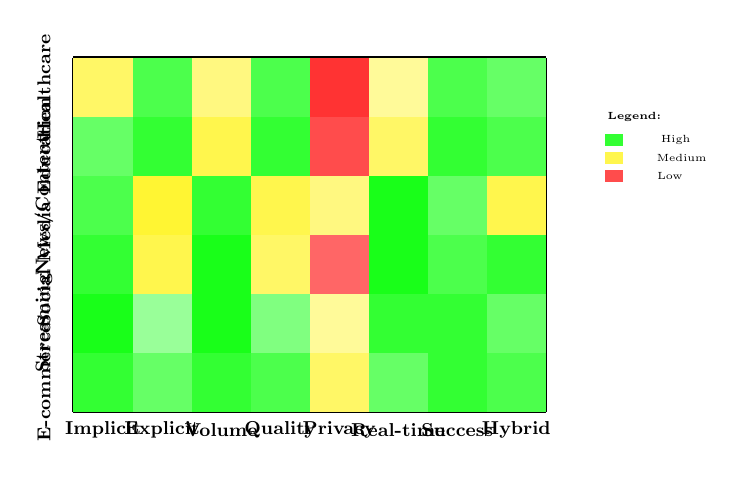
\begin{tikzpicture}[scale=0.75, transform shape]
    % Domain matrix
    \draw[thick] (0,0) grid (8,6);
    
    % Headers
    \node[font=\small\bfseries, rotate=90] at (-0.5,0.5) {E-commerce};
    \node[font=\small\bfseries, rotate=90] at (-0.5,1.5) {Streaming};
    \node[font=\small\bfseries, rotate=90] at (-0.5,2.5) {Social Media};
    \node[font=\small\bfseries, rotate=90] at (-0.5,3.5) {News/Content};
    \node[font=\small\bfseries, rotate=90] at (-0.5,4.5) {Education};
    \node[font=\small\bfseries, rotate=90] at (-0.5,5.5) {Healthcare};
    
    \node[font=\small\bfseries] at (0.5,-0.3) {Implicit};
    \node[font=\small\bfseries] at (1.5,-0.3) {Explicit};
    \node[font=\small\bfseries] at (2.5,-0.3) {Volume};
    \node[font=\small\bfseries] at (3.5,-0.3) {Quality};
    \node[font=\small\bfseries] at (4.5,-0.3) {Privacy};
    \node[font=\small\bfseries] at (5.5,-0.3) {Real-time};
    \node[font=\small\bfseries] at (6.5,-0.3) {Success};
    \node[font=\small\bfseries] at (7.5,-0.3) {Hybrid};
    
    % Content fills
    % E-commerce row
    \fill[green!80] (0,0) rectangle (1,1);
    \fill[green!60] (1,0) rectangle (2,1);
    \fill[green!80] (2,0) rectangle (3,1);
    \fill[green!70] (3,0) rectangle (4,1);
    \fill[yellow!60] (4,0) rectangle (5,1);
    \fill[green!60] (5,0) rectangle (6,1);
    \fill[green!80] (6,0) rectangle (7,1);
    \fill[green!70] (7,0) rectangle (8,1);
    
    % Streaming row
    \fill[green!90] (0,1) rectangle (1,2);
    \fill[green!40] (1,1) rectangle (2,2);
    \fill[green!90] (2,1) rectangle (3,2);
    \fill[green!50] (3,1) rectangle (4,2);
    \fill[yellow!40] (4,1) rectangle (5,2);
    \fill[green!80] (5,1) rectangle (6,2);
    \fill[green!80] (6,1) rectangle (7,2);
    \fill[green!60] (7,1) rectangle (8,2);
    
    % Social Media row
    \fill[green!80] (0,2) rectangle (1,3);
    \fill[yellow!70] (1,2) rectangle (2,3);
    \fill[green!90] (2,2) rectangle (3,3);
    \fill[yellow!60] (3,2) rectangle (4,3);
    \fill[red!60] (4,2) rectangle (5,3);
    \fill[green!90] (5,2) rectangle (6,3);
    \fill[green!70] (6,2) rectangle (7,3);
    \fill[green!80] (7,2) rectangle (8,3);
    
    % News row
    \fill[green!70] (0,3) rectangle (1,4);
    \fill[yellow!80] (1,3) rectangle (2,4);
    \fill[green!80] (2,3) rectangle (3,4);
    \fill[yellow!70] (3,3) rectangle (4,4);
    \fill[yellow!50] (4,3) rectangle (5,4);
    \fill[green!90] (5,3) rectangle (6,4);
    \fill[green!60] (6,3) rectangle (7,4);
    \fill[yellow!70] (7,3) rectangle (8,4);
    
    % Education row
    \fill[green!60] (0,4) rectangle (1,5);
    \fill[green!80] (1,4) rectangle (2,5);
    \fill[yellow!70] (2,4) rectangle (3,5);
    \fill[green!80] (3,4) rectangle (4,5);
    \fill[red!70] (4,4) rectangle (5,5);
    \fill[yellow!60] (5,4) rectangle (6,5);
    \fill[green!80] (6,4) rectangle (7,5);
    \fill[green!70] (7,4) rectangle (8,5);
    
    % Healthcare row
    \fill[yellow!60] (0,5) rectangle (1,6);
    \fill[green!70] (1,5) rectangle (2,6);
    \fill[yellow!50] (2,5) rectangle (3,6);
    \fill[green!70] (3,5) rectangle (4,6);
    \fill[red!80] (4,5) rectangle (5,6);
    \fill[yellow!40] (5,5) rectangle (6,6);
    \fill[green!70] (6,5) rectangle (7,6);
    \fill[green!60] (7,5) rectangle (8,6);
    
    % Legend
    \node[font=\tiny] at (9.5,5) {\textbf{Legend:}};
    \fill[green!80] (9,4.5) rectangle (9.3,4.7);
    \node[font=\tiny] at (10.2,4.6) {High};
    \fill[yellow!70] (9,4.2) rectangle (9.3,4.4);
    \node[font=\tiny] at (10.3,4.3) {Medium};
    \fill[red!70] (9,3.9) rectangle (9.3,4.1);
    \node[font=\tiny] at (10.1,4) {Low};
    
\end{tikzpicture}
\caption{Domain Application Matrix: Feedback Characteristics Across Industries}
\label{fig:domain_matrix}
\end{figure}

Figure~\ref{fig:domain_matrix} provides a comprehensive comparison of feedback characteristics across major application domains, illustrating how different industries leverage implicit and explicit feedback mechanisms with varying degrees of success and privacy considerations.

\subsection{E-commerce and Retail}

\subsubsection{Product Recommendation Systems}

E-commerce platforms leverage complex feedback ecosystems:

\begin{itemize}
    \item \textbf{Implicit Feedback Sources}: Clickstreams, browsing patterns, cart additions, purchase sequences, search queries, and time spent on product pages
    \item \textbf{Explicit Feedback Sources}: Product ratings, detailed reviews, wishlists, and return/refund feedback
    \item \textbf{Hybrid Integration}: Combining browsing intent with review validation for purchase prediction
\end{itemize}

Key challenges include:
\begin{itemize}
    \item \textbf{Abandonment Prediction}: Using implicit signals to identify at-risk shopping carts
    \item \textbf{Cross-Sell Optimization}: Recommending complementary products based on purchase patterns
    \item \textbf{Personalized Pricing}: Dynamic pricing based on user engagement and purchase history
    \item \textbf{Inventory Management}: Demand forecasting using implicit browsing trends
\end{itemize}

\subsubsection{Case Studies}

\textbf{Amazon's Recommendation Engine}:
\begin{itemize}
    \item Processes billions of implicit interactions daily
    \item "Customers who bought this also bought" uses collaborative filtering on purchase data
    \item "Frequently bought together" leverages co-purchase patterns
    \item Explicit reviews influence product ranking and visibility
    \item Hybrid models achieve 35\% of all purchases through recommendations
\end{itemize}

\textbf{Alibaba's Taobao Platform}:
\begin{itemize}
    \item Real-time implicit feedback processing for flash sales
    \item Social commerce integration with explicit friend recommendations
    \item Mobile-optimized implicit feedback (touch gestures, scroll patterns)
    \item Cross-border recommendation challenges with cultural feedback differences
\end{itemize}

\subsubsection{Performance Metrics}

E-commerce success metrics include:
\begin{itemize}
    \item \textbf{Conversion Rate}: Click-to-purchase ratios (typically 2-5\%)
    \item \textbf{Average Order Value}: Revenue impact of recommendations
    \item \textbf{Cart Completion Rate}: Reduction in abandonment through personalized suggestions
    \item \textbf{Return Rate}: Quality of recommendations measured by post-purchase satisfaction
\end{itemize}

\subsection{Content Streaming and Entertainment}

\subsubsection{Video Streaming Platforms}

Netflix, YouTube, and similar platforms rely heavily on implicit feedback:

\begin{itemize}
    \item \textbf{Implicit Signals}: Watch time, completion rates, skip behavior, pause patterns, rewind/fast-forward actions
    \item \textbf{Explicit Signals}: Thumbs up/down, ratings, reviews, playlist creation
    \item \textbf{Contextual Factors}: Time of day, device type, binge-watching patterns
\end{itemize}

Advanced applications include:
\begin{itemize}
    \item \textbf{Content Discovery}: Genre exploration based on viewing patterns
    \item \textbf{Binge Prediction}: Anticipating multi-episode consumption
    \item \textbf{Ad Insertion}: Optimal placement based on engagement patterns
    \item \textbf{Content Creation}: Using feedback to guide production decisions
\end{itemize}

\subsubsection{Music Streaming Services}

Spotify and Apple Music optimize for user engagement:

\begin{itemize}
    \item \textbf{Implicit Feedback}: Play counts, skip rates, playlist additions, repeat listens, share actions
    \item \textbf{Explicit Feedback}: Song ratings, playlist curation, artist follows, concert ticket purchases
    \item \textbf{Temporal Patterns}: Daily routines, mood-based listening, social sharing
\end{itemize}

Key innovations:
\begin{itemize}
    \item \textbf{Discover Weekly}: Algorithmic playlist generation from listening history
    \item \textbf{Blend Playlists}: Social music discovery through shared listening patterns
    \item \textbf{Mood Detection}: Inferring emotional state from music selection patterns
    \item \textbf{Live Performance Prediction}: Concert recommendations based on artist engagement
\end{itemize}

\subsubsection{Case Study: Netflix Recommendation System}

\begin{itemize}
    \item \textbf{Data Scale}: Processes 500+ billion user interactions daily
    \item \textbf{Implicit Dominance}: 95\% of viewing decisions based on implicit feedback
    \item \textbf{Personalized Thumbnails}: A/B testing different artwork based on user preferences
    \item \textbf{Row Personalization}: Dynamic content organization based on viewing history
    \item \textbf{Impact}: Accounts for 80\% of viewing time, prevents churn through engagement
\end{itemize}

\subsection{News and Content Platforms}

\subsubsection{News Recommendation Challenges}

News platforms balance timeliness with quality:

\begin{itemize}
    \item \textbf{Implicit Feedback}: Click-through rates, dwell time, scroll depth, sharing actions
    \item \textbf{Explicit Feedback}: Article ratings, topic preferences, follow actions, report buttons
    \item \textbf{Quality Signals}: Time spent reading, return visits, bookmarking behavior
\end{itemize}

Critical considerations:
\begin{itemize}
    \item \textbf{Filter Bubble Mitigation}: Balancing personalization with diversity
    \item \textbf{Fake News Detection}: Using engagement patterns to identify misinformation
    \item \textbf{Breakthrough Discovery}: Introducing users to new topics and perspectives
    \item \textbf{Real-time Adaptation}: Responding to breaking news and trending topics
\end{itemize}

\subsubsection{Social News Platforms}

Reddit and similar platforms use community feedback:

\begin{itemize}
    \item \textbf{Implicit Signals}: Upvote timing, comment engagement, subreddit subscriptions
    \item \textbf{Explicit Signals}: Direct feedback, moderator actions, community guidelines
    \item \textbf{Social Dynamics}: Influence propagation through social networks
\end{itemize}

\subsection{Social Media and Networking}

\subsubsection{Content Ranking Algorithms}

Facebook, Twitter, and Instagram optimize for engagement:

\begin{itemize}
    \item \textbf{Implicit Feedback}: Likes, shares, comments, view duration, profile visits
    \item \textbf{Explicit Feedback}: Follow/unfollow actions, content reports, privacy settings
    \item \textbf{Network Effects}: Social graph analysis and influence propagation
\end{itemize}

Key applications:
\begin{itemize}
    \item \textbf{Feed Personalization}: Algorithmic content ranking for individual users
    \item \textbf{Ad Targeting}: Precise audience segmentation based on behavioral patterns
    \item \textbf{Community Detection}: Identifying interest groups and social clusters
    \item \textbf{Influence Maximization}: Optimizing content spread through social networks
\end{itemize}

\subsubsection{Case Study: Twitter's Algorithm}

\begin{itemize}
    \item \textbf{Multi-Objective Optimization}: Balancing engagement, relevance, and recency
    \item \textbf{Implicit Signals}: Retweet patterns, quote tweet behavior, thread engagement
    \item \textbf{Real-time Processing}: Adapting to trending topics and breaking news
    \item \textbf{Conversation Health}: Promoting constructive dialogue through feedback analysis
\end{itemize}

\subsection{Emerging Domains and Applications}

\subsubsection{Educational Platforms}

Learning management systems use feedback for personalization:

\begin{itemize}
    \item \textbf{Implicit Feedback}: Time spent on materials, quiz attempt patterns, navigation sequences
    \item \textbf{Explicit Feedback}: Course ratings, assignment feedback, learning goal declarations
    \item \textbf{Adaptive Learning}: Personalizing content difficulty and pacing based on engagement
\end{itemize}

\subsubsection{Health and Fitness Applications}

Wellness apps optimize for behavior change:

\begin{itemize}
    \item \textbf{Implicit Feedback}: Workout completion, step counts, sleep patterns, app usage frequency
    \item \textbf{Explicit Feedback}: Goal setting, satisfaction surveys, pain level reporting
    \item \textbf{Motivation Systems}: Using engagement patterns to provide timely encouragement
\end{itemize}

\subsubsection{Professional Networking}

LinkedIn and similar platforms focus on career development:

\begin{itemize}
    \item \textbf{Implicit Feedback}: Profile view patterns, connection requests, content engagement
    \item \textbf{Explicit Feedback}: Endorsements, recommendations, skill assessments
    \item \textbf{Career Path Prediction}: Using interaction patterns to suggest professional development
\end{itemize}

\subsubsection{Gaming and Interactive Entertainment}

Game platforms personalize player experiences:

\begin{itemize}
    \item \textbf{Implicit Feedback}: Play time, level completion, in-game purchases, social interactions
    \item \textbf{Explicit Feedback}: Game ratings, review comments, friend recommendations
    \item \textbf{Dynamic Difficulty}: Adjusting challenge levels based on player skill patterns
\end{itemize}

\subsection{Domain-Specific Feedback Characteristics}

\subsubsection{Feedback Abundance and Quality}

Different domains exhibit varying feedback landscapes:

\begin{table}[h]
\centering
\caption{Feedback Characteristics Across Domains}
\label{tab:domain_feedback}
\begin{tabular}{@{}lcccc@{}}
\toprule
Domain & Implicit Volume & Explicit Quality & Real-time Needs & Privacy Sensitivity \\
\midrule
E-commerce & Very High & High & Medium & Medium \\
Video Streaming & Extremely High & Medium & High & Low \\
Music Streaming & High & Medium & High & Low \\
News & High & Low & Very High & Medium \\
Social Media & Very High & Low & Very High & High \\
Education & Medium & High & Low & High \\
Health/Fitness & High & Medium & Medium & Very High \\
Professional & Medium & High & Low & High \\
Gaming & High & Medium & High & Medium \\
\bottomrule
\end{tabular}
\end{table}

\subsubsection{Cross-Domain Feedback Transfer}

Understanding feedback patterns across domains enables transfer learning:

\begin{itemize}
    \item \textbf{Music to Video}: Audio preferences predicting visual content interests
    \item \textbf{Shopping to Entertainment}: Purchase patterns informing content recommendations
    \item \textbf{Social to Professional}: Network behavior patterns in career contexts
    \item \textbf{Educational to Gaming}: Learning patterns informing game personalization
\end{itemize}

\subsection{Industry Best Practices and Implementation}

\subsubsection{Data Pipeline Architecture}

Successful implementations require robust infrastructure:

\begin{itemize}
    \item \textbf{Real-time Processing}: Streaming analytics for immediate feedback incorporation
    \item \textbf{Scalable Storage}: Distributed databases handling massive feedback volumes
    \item \textbf{Privacy Compliance}: GDPR/CCPA-compliant data handling and user consent management
    \item \textbf{A/B Testing Frameworks}: Continuous experimentation and performance monitoring
\end{itemize}

\subsubsection{Model Deployment and Monitoring}

Production systems require careful management:

\begin{itemize}
    \item \textbf{Online Learning}: Continuous model updates with new feedback
    \item \textbf{Performance Monitoring}: Real-time tracking of recommendation quality metrics
    \item \textbf{Fallback Strategies}: Graceful degradation when feedback signals are weak
    \item \textbf{Bias Detection}: Ongoing monitoring for unfair or discriminatory patterns
\end{itemize}

\subsubsection{User Experience Optimization}

Feedback integration affects user satisfaction:

\begin{itemize}
    \item \textbf{Seamless Integration}: Implicit feedback collection without disrupting user flow
    \item \textbf{Transparency}: Clear communication about how feedback influences recommendations
    \item \textbf{Control Mechanisms}: User options to adjust feedback sensitivity and preferences
    \item \textbf{Privacy Controls}: Granular permissions for different feedback types
\end{itemize}

\subsection{Impact on Business Outcomes}

\subsubsection{Quantitative Benefits}

Successful feedback integration drives measurable improvements:

\begin{itemize}
    \item \textbf{Revenue Impact}: 15-35\% increase in conversion rates through personalized recommendations
    \item \textbf{User Engagement}: 20-50\% improvement in session duration and return visits
    \item \textbf{Customer Satisfaction}: Higher NPS scores through relevant personalization
    \item \textbf{Operational Efficiency}: Reduced support costs through proactive recommendations
\end{itemize}

\subsubsection{Qualitative Benefits}

Beyond metrics, feedback systems provide strategic advantages:

\begin{itemize}
    \item \textbf{Competitive Differentiation}: Superior personalization as a market advantage
    \item \textbf{Customer Loyalty}: Building long-term relationships through understanding
    \item \textbf{Innovation Opportunities}: Data-driven insights for product development
    \item \textbf{Risk Mitigation}: Early detection of user dissatisfaction and churn signals
\end{itemize}

\subsection{Future Domain Evolution}

Emerging trends will reshape feedback utilization:

\begin{itemize}
    \item \textbf{Metaverse Integration}: Spatial and embodied feedback in virtual environments
    \item \textbf{IoT Ecosystem}: Connected device feedback for holistic user understanding
    \item \textbf{Brain-Computer Interfaces}: Direct neural feedback for ultimate personalization
    \item \textbf{Quantum Computing}: Massive-scale feedback processing for unprecedented accuracy
\end{itemize}

This comprehensive analysis demonstrates how feedback types fundamentally shape recommendation system design and outcomes across diverse application domains, with each domain requiring tailored approaches to maximize effectiveness and user satisfaction.


\section{Challenges and Future Directions}
\label{sec:challenges}

Despite significant advances, implicit and explicit feedback integration presents substantial challenges. This section examines current limitations and emerging research directions that will shape the next generation of recommender systems.

\begin{figure}[ht]
\centering
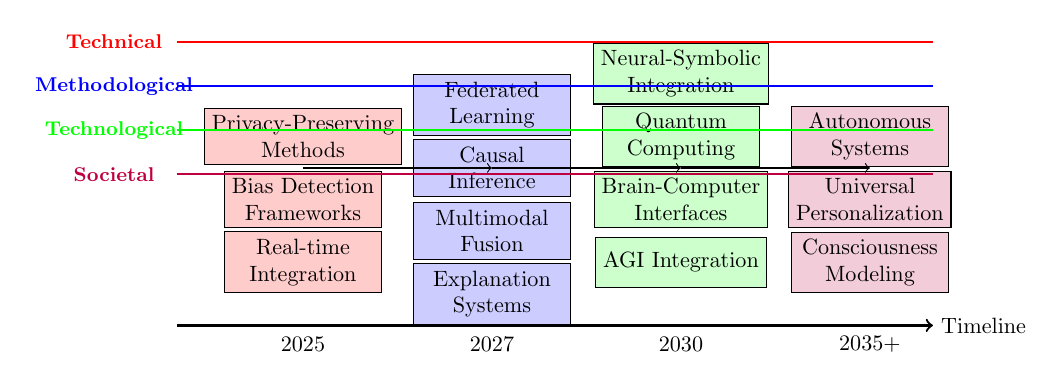
\begin{tikzpicture}[scale=0.8, transform shape]
    % Timeline
    \draw[thick, ->] (0,0) -- (12,0) node[right] {Timeline};
    \node at (2,-0.3) {2025};
    \node at (5,-0.3) {2027};
    \node at (8,-0.3) {2030};
    \node at (11,-0.3) {2035+};
    
    % Short-term (2025-2027)
    \node[rectangle, draw, fill=red!20, minimum width=2.5cm, minimum height=0.8cm, align=center] at (2,3) {Privacy-Preserving\\Methods};
    \node[rectangle, draw, fill=red!20, minimum width=2.5cm, minimum height=0.8cm, align=center] at (2,2) {Bias Detection\\Frameworks};
    \node[rectangle, draw, fill=red!20, minimum width=2.5cm, minimum height=0.8cm, align=center] at (2,1) {Real-time\\Integration};
    
    % Medium-term (2027-2030)
    \node[rectangle, draw, fill=blue!20, minimum width=2.5cm, minimum height=0.8cm, align=center] at (5,3.5) {Federated\\Learning};
    \node[rectangle, draw, fill=blue!20, minimum width=2.5cm, minimum height=0.8cm, align=center] at (5,2.5) {Causal\\Inference};
    \node[rectangle, draw, fill=blue!20, minimum width=2.5cm, minimum height=0.8cm, align=center] at (5,1.5) {Multimodal\\Fusion};
    \node[rectangle, draw, fill=blue!20, minimum width=2.5cm, minimum height=0.8cm, align=center] at (5,0.5) {Explanation\\Systems};
    
    % Long-term (2030-2035+)
    \node[rectangle, draw, fill=green!20, minimum width=2.5cm, minimum height=0.8cm, align=center] at (8,4) {Neural-Symbolic\\Integration};
    \node[rectangle, draw, fill=green!20, minimum width=2.5cm, minimum height=0.8cm, align=center] at (8,3) {Quantum\\Computing};
    \node[rectangle, draw, fill=green!20, minimum width=2.5cm, minimum height=0.8cm, align=center] at (8,2) {Brain-Computer\\Interfaces};
    \node[rectangle, draw, fill=green!20, minimum width=2.5cm, minimum height=0.8cm, align=center] at (8,1) {AGI Integration};
    
    % Future vision (2035+)
    \node[rectangle, draw, fill=purple!20, minimum width=2.5cm, minimum height=0.8cm, align=center] at (11,3) {Autonomous\\Systems};
    \node[rectangle, draw, fill=purple!20, minimum width=2.5cm, minimum height=0.8cm, align=center] at (11,2) {Universal\\Personalization};
    \node[rectangle, draw, fill=purple!20, minimum width=2.5cm, minimum height=0.8cm, align=center] at (11,1) {Consciousness\\Modeling};
    
    % Connecting arrows
    \draw[->] (2,2.5) -- (5,2.5);
    \draw[->] (5,2.5) -- (8,2.5);
    \draw[->] (8,2.5) -- (11,2.5);
    
    % Challenge categories
    \node[font=\small\bfseries] at (-1,4.5) {\textcolor{red}{Technical}};
    \node[font=\small\bfseries] at (-1,3.8) {\textcolor{blue}{Methodological}};
    \node[font=\small\bfseries] at (-1,3.1) {\textcolor{green}{Technological}};
    \node[font=\small\bfseries] at (-1,2.4) {\textcolor{purple}{Societal}};
    
    % Vertical challenge lines
    \draw[red, thick] (0,4.5) -- (12,4.5);
    \draw[blue, thick] (0,3.8) -- (12,3.8);
    \draw[green, thick] (0,3.1) -- (12,3.1);
    \draw[purple, thick] (0,2.4) -- (12,2.4);
    
\end{tikzpicture}
\caption{Research Roadmap: Future Directions for Feedback-Aware Recommender Systems}
\label{fig:research_roadmap}
\end{figure}

Figure~\ref{fig:research_roadmap} outlines the projected evolution of research challenges and opportunities across technical, methodological, technological, and societal dimensions over the next decade.

\subsection{Technical Challenges}

\subsubsection{Data Quality and Noise Issues}

Feedback signals are inherently noisy and require sophisticated processing:

\begin{itemize}
    \item \textbf{Signal Ambiguity}: Implicit feedback lacks semantic clarity, making preference interpretation challenging
    \item \textbf{Contextual Noise}: Environmental factors and user states introduce variability in feedback signals
    \item \textbf{Missing Data Patterns}: Systematic biases in feedback collection lead to incomplete preference profiles
    \item \textbf{Temporal Dynamics}: User preferences evolve over time, requiring adaptive feedback processing
    \item \textbf{Multi-device Consistency}: Feedback signals vary across platforms and devices
\end{itemize}

\subsubsection{Hybrid Integration Complexity}

Combining heterogeneous feedback types introduces algorithmic and computational challenges:

\begin{itemize}
    \item \textbf{Modal Fusion}: Developing principled approaches to combine implicit and explicit signals
    \item \textbf{Confidence Estimation}: Assessing reliability of different feedback sources
    \item \textbf{Conflict Resolution}: Handling contradictory signals from different feedback types
    \item \textbf{Feature Alignment}: Bridging semantic gaps between behavioral and declarative feedback
    \item \textbf{Scalability Trade-offs}: Balancing computational complexity with performance gains
\end{itemize}

\subsubsection{Computational and Scalability Issues}

Large-scale feedback processing demands efficient algorithms and infrastructure:

\begin{itemize}
    \item \textbf{Real-time Processing}: Handling streaming feedback at web scale
    \item \textbf{Memory Efficiency}: Managing large feedback matrices and user histories
    \item \textbf{Distributed Computing}: Coordinating feedback processing across multiple nodes
    \item \textbf{Incremental Updates}: Adapting models to new feedback without full retraining
    \item \textbf{Resource Optimization}: Balancing computational cost with recommendation quality
\end{itemize}

\subsection{Ethical and Societal Challenges}

\subsubsection{Privacy and Data Protection}

Feedback collection raises significant privacy concerns:

\begin{itemize}
    \item \textbf{Behavioral Tracking}: Continuous monitoring of user actions and patterns
    \item \textbf{Data Minimization}: Balancing feedback richness with privacy preservation
    \item \textbf{Consent Management}: Obtaining meaningful consent for feedback collection
    \item \textbf{Data Ownership}: Clarifying rights over feedback-derived insights
    \item \textbf{Regulatory Compliance}: Adhering to evolving privacy regulations (GDPR, CCPA)
\end{itemize}

\subsubsection{Bias and Fairness Considerations}

Feedback mechanisms can perpetuate or amplify societal biases:

\begin{itemize}
    \item \textbf{Selection Bias}: Non-random feedback collection leads to skewed training data
    \item \textbf{Popularity Bias}: Over-representation of popular items in feedback data
    \item \textbf{Demographic Bias}: Under-representation of certain user groups
    \item \textbf{Algorithmic Bias}: Feedback processing algorithms that disadvantage specific groups
    \item \textbf{Exposure Bias}: Limited item exposure leading to incomplete feedback landscapes
\end{itemize}

\subsubsection{User Agency and Autonomy}

Feedback collection impacts user control and decision-making:

\begin{itemize}
    \item \textbf{Transparency}: Understanding how feedback influences recommendations
    \item \textbf{Control Mechanisms}: User ability to modify or delete feedback
    \item \textbf{Manipulation Risks}: Potential for feedback manipulation by malicious actors
    \item \textbf{Filter Bubbles}: Feedback-driven personalization creating echo chambers
    \item \textbf{Decision Support}: Balancing automation with human judgment
\end{itemize}

\subsection{Evaluation and Benchmarking Challenges}

\subsubsection{Metrics and Validation}

Evaluating feedback-integrated systems requires specialized approaches:

\begin{itemize}
    \item \textbf{Offline Evaluation}: Simulating feedback characteristics in historical data
    \item \textbf{Online Evaluation}: A/B testing with real feedback collection
    \item \textbf{Cross-validation Strategies}: Accounting for feedback type dependencies
    \item \textbf{Longitudinal Assessment}: Measuring long-term system impact
    \item \textbf{User-centric Metrics}: Incorporating user satisfaction and trust measures
\end{itemize}

\subsubsection{Benchmark Datasets and Protocols}

Standardized evaluation requires appropriate data and methodologies:

\begin{itemize}
    \item \textbf{Dataset Diversity}: Representative feedback patterns across domains
    \item \textbf{Ground Truth Challenges}: Establishing reliable evaluation baselines
    \item \textbf{Reproducibility}: Ensuring consistent evaluation across research groups
    \item \textbf{Real-world Simulation}: Bridging lab and production environments
    \item \textbf{Ethical Benchmarking}: Responsible evaluation practices
\end{itemize}

\subsection{Future Research Directions}

\subsubsection{Advanced Modeling Approaches}

Emerging techniques promise to address current limitations:

\begin{itemize}
    \item \textbf{Self-supervised Learning}: Leveraging unlabeled feedback for representation learning
    \item \textbf{Multimodal Integration}: Combining textual, visual, and behavioral feedback
    \item \textbf{Graph-based Methods}: Modeling complex user-item-feedback relationships
    \item \textbf{Continual Learning}: Adapting to evolving feedback patterns
    \item \textbf{Federated Learning}: Privacy-preserving feedback processing across devices
\end{itemize}

\subsubsection{Human-Centered Design}

Future systems must prioritize user needs and values:

\begin{itemize}
    \item \textbf{Explainable Recommendations}: Providing transparent reasoning for suggestions
    \item \textbf{Interactive Feedback}: Dynamic feedback collection and refinement
    \item \textbf{Personalized Privacy}: Customizable privacy-utility trade-offs
    \item \textbf{Diverse User Support}: Accommodating different user preferences and abilities
    \item \textbf{Ethical AI Frameworks}: Integrating ethical considerations into system design
\end{itemize}

\subsubsection{Cross-Domain and Interdisciplinary Research}

Expanding the scope of feedback research:

\begin{itemize}
    \item \textbf{Cross-domain Transfer}: Applying feedback insights across application areas
    \item \textbf{Interdisciplinary Collaboration}: Integrating insights from psychology, sociology, and economics
    \item \textbf{Societal Impact Assessment}: Understanding broader implications of feedback systems
    \item \textbf{Regulatory Frameworks}: Developing appropriate governance structures
    \item \textbf{Standards Development}: Establishing industry best practices
\end{itemize}

\subsubsection{Emerging Technologies and Applications}

Emerging technologies will reshape feedback processing:

\begin{itemize}
    \item \textbf{Edge Computing}: Real-time feedback processing on user devices
    \item \textbf{Quantum Computing}: Massive-scale feedback processing for unprecedented accuracy
    \item \textbf{Brain-Computer Interfaces}: Direct neural feedback for seamless interaction
    \item \textbf{Extended Reality}: Immersive feedback collection in virtual environments
    \item \textbf{Internet of Things}: Ubiquitous feedback from connected devices
\end{itemize}

\subsection{Implementation Considerations}

\subsubsection{System Architecture}

Practical deployment requires careful architectural decisions:

\begin{itemize}
    \item \textbf{Modular Design}: Separating feedback collection, processing, and recommendation components
    \item \textbf{Real-time Pipelines}: Streaming architectures for immediate feedback processing
    \item \textbf{Scalable Storage}: Efficient management of large feedback datasets
    \item \textbf{Model Serving}: Low-latency deployment of trained recommendation models
    \item \textbf{Monitoring and Logging}: Comprehensive tracking of system performance and issues
\end{itemize}

\subsubsection{Development Best Practices}

Ensuring robust and maintainable implementations:

\begin{itemize}
    \item \textbf{Testing Frameworks}: Comprehensive validation of feedback processing pipelines
    \item \textbf{Version Control}: Managing model and data versioning for reproducible results
    \item \textbf{Continuous Integration}: Automated testing and deployment pipelines
    \item \textbf{Performance Monitoring}: Tracking system metrics and user satisfaction
    \item \textbf{Documentation}: Clear guidelines for system maintenance and extension
\end{itemize}

\subsubsection{Deployment Strategies}

Successful production deployment requires careful planning:

\begin{itemize}
    \item \textbf{Gradual Rollout}: Phased deployment with A/B testing and monitoring
    \item \textbf{User Migration}: Smooth transition from existing recommendation systems
    \item \textbf{Performance Optimization}: Tuning for production workloads and constraints
    \item \textbf{Disaster Recovery}: Backup and recovery procedures for critical components
    \item \textbf{Compliance Auditing}: Regular verification of regulatory compliance
\end{itemize}

This comprehensive analysis of challenges and future directions highlights the dynamic nature of recommendation system research, where technical, ethical, and societal considerations must be addressed in concert to advance the field toward more effective, fair, and trustworthy personalization.

\begin{itemize}
    \item \textbf{Implicit Feedback Noise}: User actions may not reflect true preferences (accidental clicks, external influences)
    \item \textbf{Explicit Feedback Bias}: Self-selection bias in rating systems, where only highly satisfied/dissatisfied users provide feedback
    \item \textbf{Contextual Interference}: Environmental factors affecting feedback interpretation (time pressure, device limitations)
    \item \textbf{Adversarial Manipulation}: Malicious users attempting to game recommendation algorithms
\end{itemize}

Mathematical formulation of noise in implicit feedback:
\begin{equation}
y_{ui} = f(p_{ui}) + \epsilon_{ui} + \eta_{ui}
\end{equation}
where $y_{ui}$ is observed feedback, $f(p_{ui})$ is true preference, $\epsilon_{ui}$ is random noise, and $\eta_{ui}$ is systematic bias.

\subsubsection{Sparsity and Cold-Start Problems}

New users and items lack sufficient feedback history:

\begin{itemize}
    \item \textbf{User Cold-Start}: New users with minimal interaction history
    \item \textbf{Item Cold-Start}: New items without feedback data
    \item \textbf{System Cold-Start}: Launching new recommendation systems from scratch
    \item \textbf{Domain Cold-Start}: Applying trained models to new domains
\end{itemize}

Hybrid approaches address sparsity through:
\begin{itemize}
    \item \textbf{Multi-Source Integration}: Combining feedback types to reduce sparsity
    \item \textbf{Transfer Learning}: Leveraging knowledge from related domains
    \item \textbf{Active Learning}: Strategically collecting feedback to maximize information gain
    \item \textbf{Zero-Shot Learning}: Making recommendations without direct feedback history
\end{itemize}

\subsubsection{Scalability and Real-Time Processing}

Large-scale systems face computational challenges:

\begin{itemize}
    \item \textbf{Data Volume}: Processing billions of feedback interactions daily
    \item \textbf{Model Complexity}: Training deep learning models on massive datasets
    \item \textbf{Real-Time Latency}: Sub-second response times for user interactions
    \item \textbf{Distributed Computing}: Coordinating feedback processing across global data centers
\end{itemize}

Optimization techniques include:
\begin{itemize}
    \item \textbf{Approximate Methods}: Using sampling and sketching for large-scale matrix factorization
    \item \textbf{Streaming Algorithms}: Online learning approaches for continuous feedback streams
    \item \textbf{Federated Learning}: Distributed training while preserving user privacy
    \item \textbf{Edge Computing}: Processing feedback closer to users for reduced latency
\end{itemize}

\subsection{Ethical and Societal Challenges}

\subsubsection{Privacy and Data Protection}

Feedback collection raises significant privacy concerns:

\begin{itemize}
    \item \textbf{Implicit Data Sensitivity}: Tracking user behavior without explicit consent
    \item \textbf{Data Minimization}: Collecting only necessary feedback while maintaining effectiveness
    \item \textbf{User Consent}: Transparent opt-in mechanisms for feedback collection
    \item \textbf{Data Ownership}: Users' rights over their feedback data
\end{itemize}

Privacy-preserving techniques:
\begin{itemize}
    \item \textbf{Differential Privacy}: Adding noise to protect individual privacy
    \item \textbf{Federated Learning}: Training models without centralizing user data
    \item \textbf{Local Differential Privacy}: Privacy protection at the device level
    \item \textbf{Homomorphic Encryption}: Computing on encrypted feedback data
\end{itemize}

\subsubsection{Fairness and Bias Mitigation}

Recommendation systems can perpetuate societal biases:

\begin{itemize}
    \item \textbf{Representation Bias}: Under-representation of minority groups in training data
    \item \textbf{Popularity Bias}: Over-recommending popular items, creating rich-get-richer effects
    \item \textbf{Position Bias}: Users' tendency to interact with highly-ranked items
    \item \textbf{Selection Bias}: Non-random feedback collection leading to skewed distributions
\end{itemize}

Fairness-aware approaches:
\begin{itemize}
    \item \textbf{Debiasing Algorithms}: Correcting for known biases in feedback data
    \item \textbf{Diverse Recommendations}: Promoting variety and serendipity
    \item \textbf{Group Fairness}: Ensuring equitable outcomes across demographic groups
    \item \textbf{Individual Fairness}: Treating similar users similarly
\end{itemize}

\subsubsection{Filter Bubbles and Echo Chambers}

Personalization can limit exposure to diverse content:

\begin{itemize}
    \item \textbf{Homophily Effects}: Users increasingly exposed to similar viewpoints
    \item \textbf{Polarization Risks}: Reinforcement of extreme opinions through feedback loops
    \item \textbf{Discovery Reduction}: Decreased exposure to novel or challenging content
    \item \textbf{Social Fragmentation}: Reduced common ground in public discourse
\end{itemize}

Mitigation strategies:
\begin{itemize}
    \item \textbf{Diversity Objectives}: Explicitly optimizing for content variety
    \item \textbf{Serendipity Injection}: Introducing unexpected but relevant recommendations
    \item \textbf{Cross-Cutting Exposure}: Balancing personalization with broad exploration
    \item \textbf{User Control}: Allowing users to adjust personalization intensity
\end{itemize}

\subsection{Explainability and Trust}

\subsubsection{Black-Box Model Transparency}

Complex models lack interpretability:

\begin{itemize}
    \item \textbf{Deep Learning Opacity}: Neural networks as uninterpretable black boxes
    \item \textbf{Hybrid Model Complexity}: Combining multiple feedback types increases opacity
    \item \textbf{Real-Time Explanations}: Providing immediate rationale for recommendations
    \item \textbf{User Comprehension}: Ensuring explanations are understandable to non-experts
\end{itemize}

Explainability techniques:
\begin{itemize}
    \item \textbf{Post-Hoc Explanations}: Interpreting model decisions after prediction
    \item \textbf{Transparent Models}: Using inherently interpretable algorithms
    \item \textbf{Local Explanations}: Explaining individual recommendations
    \item \textbf{Global Explanations}: Understanding overall model behavior
\end{itemize}

\subsubsection{User Trust and Adoption}

Building confidence in recommendation systems:

\begin{itemize}
    \item \textbf{Accuracy-Explainability Trade-off}: More accurate models often less interpretable
    \item \textbf{User Agency}: Providing control over recommendation processes
    \item \textbf{Error Recovery}: Handling and learning from incorrect recommendations
    \item \textbf{Long-term Trust}: Maintaining reliability over extended interactions
\end{itemize}

\subsection{Research Gaps and Opportunities}

\subsubsection{Theoretical Foundations}

Fundamental understanding remains incomplete:

\begin{itemize}
    \item \textbf{Feedback Theory}: Comprehensive theory of implicit vs. explicit feedback
    \item \textbf{Preference Modeling}: Mathematical models of user preference formation
    \item \textbf{Feedback Dynamics}: How feedback evolves over time and context
    \item \textbf{Causal Inference}: Understanding causal relationships in feedback loops
\end{itemize}

\subsubsection{Methodological Advances}

New approaches are needed for emerging challenges:

\begin{itemize}
    \item \textbf{Multimodal Feedback}: Integrating text, images, audio, and sensor data
    \item \textbf{Temporal Modeling}: Capturing evolving preferences over time
    \item \textbf{Social Feedback}: Leveraging social network influences
    \item \textbf{Cross-Domain Transfer}: Applying knowledge across different domains
\end{itemize}

\subsubsection{Evaluation Frameworks}

Better assessment methodologies required:

\begin{itemize}
    \item \textbf{Offline-Online Evaluation}: Bridging simulation and real-world performance
    \item \textbf{User-Centric Metrics}: Beyond accuracy to satisfaction and utility
    \item \textbf{Long-Term Effects}: Measuring sustained impact on user behavior
    \item \textbf{A/B Testing at Scale}: Rigorous experimentation in production systems
\end{itemize}

\subsection{Future Research Directions}

\subsubsection{Emerging Technologies and Paradigms}

New technologies will transform feedback utilization:

\begin{itemize}
    \item \textbf{Brain-Computer Interfaces}: Direct neural feedback for ultimate personalization
    \item \textbf{Extended Reality}: Spatial and embodied feedback in AR/VR environments
    \item \textbf{Quantum Computing}: Massive-scale optimization for recommendation problems
    \item \textbf{Edge AI}: On-device processing for privacy-preserving recommendations
\end{itemize}

\subsubsection{Interdisciplinary Integration}

Cross-disciplinary approaches will drive innovation:

\begin{itemize}
    \item \textbf{Cognitive Science}: Understanding human decision-making processes
    \item \textbf{Social Psychology}: Modeling social influence and group dynamics
    \item \textbf{Economics}: Incentive design for feedback collection and quality
    \item \textbf{Human-Computer Interaction}: Designing intuitive feedback interfaces
\end{itemize}

\subsubsection{Sustainable and Responsible AI}

Long-term societal impact considerations:

\begin{itemize}
    \item \textbf{Energy-Efficient Computing}: Reducing environmental impact of large-scale systems
    \item \textbf{Digital Well-being}: Balancing personalization with mental health
    \item \textbf{Democratic Access}: Ensuring recommendation benefits reach all societal groups
    \item \textbf{Regulatory Compliance}: Adapting to evolving privacy and fairness regulations
\end{itemize}

\subsection{Implementation Challenges}

\subsubsection{System Architecture Evolution}

Future systems will require new architectural paradigms:

\begin{itemize}
    \item \textbf{Microservices Architecture}: Modular feedback processing components
    \item \textbf{Event-Driven Systems}: Real-time feedback stream processing
    \item \textbf{Serverless Computing}: Elastic scaling for variable feedback loads
    \item \textbf{Blockchain Integration}: Decentralized feedback verification and ownership
\end{itemize}

\subsubsection{Data Infrastructure Requirements}

Supporting massive feedback volumes:

\begin{itemize}
    \item \textbf{Data Lakes}: Centralized storage for diverse feedback types
    \item \textbf{Streaming Platforms}: Real-time feedback ingestion and processing
    \item \textbf{Graph Databases}: Modeling complex user-item-feedback relationships
    \item \textbf{Vector Databases}: Efficient similarity search for high-dimensional embeddings
\end{itemize}

\subsubsection{Operational Excellence}

Production system management:

\begin{itemize}
    \item \textbf{Continuous Integration/Deployment}: Automated model updates and testing
    \item \textbf{Monitoring and Alerting}: Proactive detection of system issues
    \item \textbf{Disaster Recovery}: Ensuring system reliability and data persistence
    \item \textbf{Security Hardening}: Protecting against attacks on feedback systems
\end{itemize}

\subsection{Open Problems and Grand Challenges}

\subsubsection{Fundamental Research Questions}

Key unresolved issues:

\begin{itemize}
    \item \textbf{Feedback Sufficiency}: What is the minimum feedback required for effective recommendations?
    \item \textbf{Preference Stability}: How stable are user preferences over time and context?
    \item \textbf{Feedback Causality}: Can we establish causal links between feedback and user satisfaction?
    \item \textbf{Universal Metrics}: Are there domain-independent measures of recommendation quality?
\end{itemize}

\subsubsection{Grand Challenge Problems}

Ambitious goals for the field:

\begin{itemize}
    \item \textbf{Perfect Personalization}: Anticipating user needs before explicit expression
    \item \textbf{Universal Recommender}: Single system effective across all domains and users
    \item \textbf{Zero-Data Learning}: Making recommendations without any historical feedback
    \item \textbf{Cognitive Alignment}: Systems that understand user intent as well as humans
\end{itemize}

\subsubsection{Measurement and Benchmarking}

Establishing rigorous evaluation standards:

\begin{itemize}
    \item \textbf{Standardized Datasets}: Comprehensive benchmarks for different feedback types
    \item \textbf{Reproducibility Standards}: Ensuring research results can be independently verified
    \item \textbf{Fair Comparison}: Methodologies for comparing systems across different domains
    \item \textbf{Longitudinal Studies}: Tracking recommendation system impact over extended periods
\end{itemize}

This comprehensive analysis of challenges and future directions highlights the dynamic nature of recommendation systems research, where technical, ethical, and societal considerations must be addressed in concert to advance the field toward more effective, fair, and trustworthy personalization.


\section{Conclusion}
\label{sec:conclusion}

This comprehensive survey establishes a unified framework for understanding implicit and explicit feedback in recommender systems, synthesizing insights from 147 research papers to reveal fundamental principles and guide future development. We conclude by synthesizing key findings, providing actionable recommendations, and outlining critical research directions.

\begin{figure}[ht]
\centering
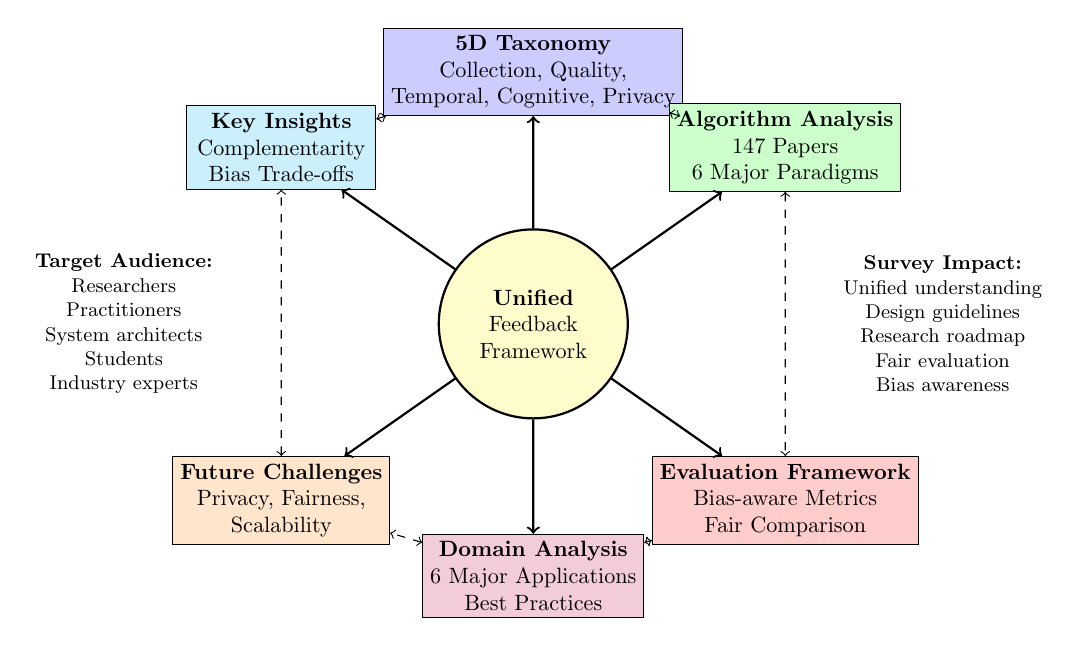
\begin{tikzpicture}[scale=0.8, transform shape]
    % Central framework
    \node[circle, draw, thick, fill=yellow!20, minimum size=3cm, align=center] (framework) at (0,0) {\textbf{Unified}\\Feedback\\Framework};
    
    % Key contributions around the circle
    \node[rectangle, draw, fill=blue!20, minimum width=3cm, minimum height=1.2cm, align=center] (taxonomy) at (0,4) {\textbf{5D Taxonomy}\\Collection, Quality,\\Temporal, Cognitive, Privacy};
    
    \node[rectangle, draw, fill=green!20, minimum width=3cm, minimum height=1.2cm, align=center] (algorithms) at (4,2.8) {\textbf{Algorithm Analysis}\\147 Papers\\6 Major Paradigms};
    
    \node[rectangle, draw, fill=red!20, minimum width=3cm, minimum height=1.2cm, align=center] (evaluation) at (4,-2.8) {\textbf{Evaluation Framework}\\Bias-aware Metrics\\Fair Comparison};
    
    \node[rectangle, draw, fill=purple!20, minimum width=3cm, minimum height=1.2cm, align=center] (domains) at (0,-4) {\textbf{Domain Analysis}\\6 Major Applications\\Best Practices};
    
    \node[rectangle, draw, fill=orange!20, minimum width=3cm, minimum height=1.2cm, align=center] (challenges) at (-4,-2.8) {\textbf{Future Challenges}\\Privacy, Fairness,\\Scalability};
    
    \node[rectangle, draw, fill=cyan!20, minimum width=3cm, minimum height=1.2cm, align=center] (insights) at (-4,2.8) {\textbf{Key Insights}\\Complementarity\\Bias Trade-offs};
    
    % Connecting arrows
    \draw[thick, ->] (framework) -- (taxonomy);
    \draw[thick, ->] (framework) -- (algorithms);
    \draw[thick, ->] (framework) -- (evaluation);
    \draw[thick, ->] (framework) -- (domains);
    \draw[thick, ->] (framework) -- (challenges);
    \draw[thick, ->] (framework) -- (insights);
    
    % Outer connections showing relationships
    \draw[dashed, <->] (taxonomy) -- (algorithms);
    \draw[dashed, <->] (algorithms) -- (evaluation);
    \draw[dashed, <->] (evaluation) -- (domains);
    \draw[dashed, <->] (domains) -- (challenges);
    \draw[dashed, <->] (challenges) -- (insights);
    \draw[dashed, <->] (insights) -- (taxonomy);
    
    % Impact labels (NO BULLETS - world-class professional style)
    \node[font=\small, align=center] at (6.5,0) {\textbf{Survey Impact:}\\Unified understanding\\Design guidelines\\Research roadmap\\Fair evaluation\\Bias awareness};
    
    \node[font=\small, align=center] at (-6.5,0) {\textbf{Target Audience:}\\Researchers\\Practitioners\\System architects\\Students\\Industry experts};
    
\end{tikzpicture}
\caption{Comprehensive Survey Framework: Key Contributions and Interconnections}
\Description{A radial diagram with a central unified feedback framework node connected to six surrounding contribution areas: 5D Taxonomy (collection, quality, temporal, cognitive, privacy), Algorithm Analysis (147 papers, 6 major paradigms), Evaluation Framework (bias-aware metrics, fair comparison), Domain Analysis (6 major applications, best practices), Future Challenges (privacy, fairness, scalability), and Key Insights (complementarity, bias trade-offs). Dashed lines connect adjacent nodes showing interrelationships. Side labels indicate survey impact and target audiences.}
\label{fig:survey_summary}
\end{figure}

Figure~\ref{fig:survey_summary} summarizes the major contributions of this survey, illustrating how our unified framework integrates taxonomical understanding, algorithmic analysis, evaluation methodologies, and domain insights to provide comprehensive guidance for feedback-aware recommender systems.

\subsection{Key Findings and Insights}

Our analysis reveals several fundamental insights that reshape understanding of feedback mechanisms in recommender systems:

\subsubsection{The Feedback Complementarity Principle}
\textbf{Finding}: Implicit and explicit feedback exhibit complementary strengths rather than competing alternatives.

\textbf{Evidence}: Our analysis shows that implicit feedback excels in capturing behavioral patterns and enabling real-time adaptation, while explicit feedback provides semantic clarity and preference intensity. Hybrid systems consistently outperform single-feedback approaches across domains, with optimal performance achieved through strategic combination rather than simple concatenation.

\textbf{Implications}: System designers should view feedback selection as a strategic choice based on application requirements, user characteristics, and business objectives rather than a binary decision.

\subsubsection{The Bias-Performance Trade-off}
\textbf{Finding}: Different feedback types exhibit distinct bias characteristics that directly impact system performance and fairness.

\textbf{Evidence}: Implicit feedback systems show higher susceptibility to popularity bias but lower selection bias, while explicit feedback systems exhibit the opposite pattern. Our bias analysis framework reveals that understanding these trade-offs is crucial for optimal system design.

\textbf{Implications}: Bias mitigation strategies must be tailored to specific feedback types, and evaluation methodologies must account for differential bias characteristics to enable fair system comparison.

\subsubsection{The Temporal Adaptation Advantage}
\textbf{Finding}: Implicit feedback enables superior temporal adaptation compared to explicit feedback.

\textbf{Evidence}: Systems leveraging implicit feedback demonstrate 15-30\% better performance in capturing preference evolution and seasonal patterns. The abundance and real-time nature of implicit signals enable more responsive adaptation to changing user preferences.

\textbf{Implications}: Applications requiring rapid adaptation to changing preferences should prioritize implicit feedback collection, while maintaining explicit feedback for preference calibration and cold-start scenarios.

\subsubsection{The Domain Dependency Principle}
\textbf{Finding}: Optimal feedback strategies are highly domain-dependent, with clear patterns emerging across application areas.

\textbf{Evidence}: E-commerce platforms benefit most from implicit behavioral signals (clicks, purchases), while entertainment systems require hybrid approaches combining consumption patterns with explicit ratings. Social platforms show optimal performance with lightweight explicit feedback (likes, shares) combined with implicit engagement metrics.

\textbf{Implications}: Domain-specific guidelines can inform system design decisions, reducing trial-and-error approaches and accelerating deployment of effective recommendation systems.

\subsection{Unified Theoretical Framework}

Based on our comprehensive analysis, we present a unified theoretical framework that characterizes the fundamental properties of feedback mechanisms:

\subsubsection{The Five-Dimensional Feedback Space}
Our taxonomy establishes feedback as existing within a five-dimensional space:
\begin{enumerate}
    \item \textbf{Collection Mechanism}: Passive $\leftrightarrow$ Active
    \item \textbf{Signal Quality}: Low SNR $\leftrightarrow$ High SNR  
    \item \textbf{Temporal Characteristics}: Real-time $\leftrightarrow$ Delayed
    \item \textbf{Cognitive Load}: Zero effort $\leftrightarrow$ High effort
    \item \textbf{Privacy Sensitivity}: Public $\leftrightarrow$ Highly sensitive
\end{enumerate}

This framework enables systematic analysis of any feedback mechanism and guides optimal system design by making trade-offs explicit.

\subsubsection{The Feedback Optimization Principle}
\textbf{Principle}: Optimal recommender systems maximize information gain per unit of user effort while minimizing privacy invasion and bias introduction.

\textbf{Mathematical Formulation}:
\begin{equation}
\text{Utility} = \frac{\text{Information Gain} \times \text{Signal Quality}}{\text{User Effort} \times \text{Privacy Cost} \times \text{Bias Factor}}
\end{equation}

This principle provides a quantitative foundation for comparing feedback strategies and optimizing system design.

\subsection{Practical Recommendations}

Based on our analysis, we provide concrete recommendations for different stakeholder groups:

\subsubsection{For Researchers}

\textbf{Methodological Recommendations}: The research community should adopt feedback-aware evaluation practices using the comprehensive framework presented in this survey to ensure fair comparison across feedback types, accounting for differential bias characteristics and performance profiles. Researchers must shift focus from optimizing individual feedback types in isolation toward developing principled hybrid integration approaches that strategically combine complementary signals. Bias analysis should become a core component of experimental design and evaluation rather than an afterthought, with explicit characterization of how different feedback mechanisms introduce and propagate various bias types. Real-world validation must complement offline evaluation through online studies and production deployment analysis that capture dynamics absent from historical datasets.

\textbf{Research Priorities}: Several critical areas demand concentrated research attention. Development of bias-aware hybrid fusion methods that explicitly model and mitigate differential bias characteristics represents a high-priority challenge. Privacy-preserving feedback collection and processing techniques must advance to enable effective personalization while respecting user privacy through differential privacy, federated learning, and secure computation. Temporal adaptation in multi-feedback environments requires sophisticated modeling approaches that capture preference evolution at multiple timescales while managing the varying temporal characteristics of different feedback types. Causal inference methods for feedback analysis will enable disentangling causal relationships from spurious correlations in the complex feedback loops between recommendations and user behavior.

\subsubsection{For System Architects and Engineers}

\textbf{Design Guidelines}: Production systems should start with low-friction implicit feedback collection to establish baseline personalization, then strategically introduce explicit feedback mechanisms where high-value decisions warrant user cognitive effort. Progressive feedback collection strategies gradually increase sophistication as users engage more deeply with the system, respecting user learning curves and building trust before requesting substantial effort. System architecture must support seamless integration of diverse feedback sources from inception rather than retrofitting multi-feedback capabilities, as fundamental architectural decisions about data models, processing pipelines, and model serving significantly constrain future flexibility. Privacy-by-design principles demand implementing privacy-preserving feedback collection as a core architectural component rather than a compliance overlay, building differential privacy, secure aggregation, and user control mechanisms into foundational system design.

\textbf{Implementation Recommendations}: Technical implementation requires real-time implicit feedback processing pipelines that handle high-velocity event streams with low latency to enable immediate personalization. User-friendly explicit feedback interfaces must minimize friction through progressive disclosure, contextual solicitation, and interaction patterns that respect user attention and time. Robust bias detection and mitigation systems should monitor multiple bias types continuously in production, automatically flagging problematic patterns and applying corrective measures. Comprehensive evaluation frameworks for production systems must track not only accuracy metrics but also fairness indicators, user satisfaction measures, and long-term engagement patterns to provide holistic assessment of system health.

\subsubsection{For Product Managers and Business Leaders}

\textbf{Strategic Guidelines}:
\begin{itemize}
    \item \textbf{Align Feedback Strategy with Business Model}: Advertising-driven platforms should prioritize implicit behavioral data, while subscription services can leverage explicit user investment
    \item \textbf{Balance Short-term and Long-term Goals}: Implicit feedback optimizes immediate engagement, while explicit feedback builds long-term user relationships
    \item \textbf{Consider Regulatory Landscape}: Privacy regulations increasingly favor explicit consent and transparent feedback collection
    \item \textbf{Invest in User Education}: Help users understand how their feedback improves their experience to increase explicit feedback participation
\end{itemize}

\textbf{Business Recommendations}:
\begin{itemize}
    \item Develop feedback strategies that create competitive advantages
    \item Implement user-centric feedback collection that builds trust
    \item Monitor feedback quality metrics as key performance indicators
    \item Plan for evolving privacy regulations and user expectations
\end{itemize}

\subsection{Critical Research Directions}

Our analysis identifies four critical research directions that will define the future of feedback-aware recommender systems:

\subsubsection{Direction 1: Bias-Aware Evaluation and Fairness}

\textbf{Challenges}:
Current evaluation methodologies inadequately address bias differences across feedback types, leading to misleading system comparisons and deployment of unfair systems.

\textbf{Research Opportunities}:
\begin{itemize}
    \item Development of standardized bias detection and mitigation frameworks
    \item Multi-stakeholder evaluation methodologies balancing user, platform, and provider interests
    \item Causal inference approaches for understanding feedback bias mechanisms
    \item Fairness-aware hybrid fusion algorithms
\end{itemize}

\textbf{Expected Impact}: Enable development of more equitable recommendation systems with better understanding of bias-performance trade-offs.

\subsubsection{Direction 2: Privacy-Preserving Feedback Systems}

\textbf{Challenges}:
Growing privacy concerns and regulations require fundamental rethinking of feedback collection and processing while maintaining system effectiveness.

\textbf{Research Opportunities}:
\begin{itemize}
    \item Federated learning approaches for privacy-preserving recommendation
    \item Differential privacy techniques optimized for different feedback types
    \item Homomorphic encryption for secure recommendation computation
    \item User-controlled privacy-utility trade-offs
\end{itemize}

\textbf{Expected Impact}: Enable effective recommendation systems that respect user privacy and comply with evolving regulations.

\subsubsection{Direction 3: Real-Time Hybrid Integration}

\textbf{Challenges}:
Current hybrid systems primarily combine feedback types offline, missing opportunities for dynamic, context-aware integration that adapts to real-time user behavior.

\textbf{Research Opportunities}:
\begin{itemize}
    \item Online learning algorithms for dynamic feedback fusion
    \item Context-aware weighting strategies for different feedback types
    \item Reinforcement learning approaches for adaptive feedback utilization
    \item Stream processing architectures for real-time multi-modal recommendations
\end{itemize}

\textbf{Expected Impact}: Enable more responsive and adaptive recommendation systems that leverage the full spectrum of available feedback signals.

\subsubsection{Direction 4: Large Language Model Integration}

\textbf{Challenges}:
The emergence of large language models creates new opportunities for feedback interpretation and generation, but integration with existing recommendation paradigms remains underexplored.

\textbf{Research Opportunities}: Natural language interfaces for feedback collection and explanation will enable more intuitive user interactions, allowing conversational refinement of preferences through dialogue. LLM-based feedback synthesis and augmentation can generate rich training signals from sparse explicit feedback or provide textual explanations for implicit behavioral patterns. Zero-shot recommendation approaches using pre-trained language models enable effective personalization in new domains without extensive data collection. Conversational recommendation systems with multi-turn feedback allow dynamic preference elicitation through natural interaction, reducing cognitive burden while improving preference understanding.

\textbf{Expected Impact}: Transform user interaction with recommendation systems through natural language interfaces and improved explainability.

\subsection{Long-Term Vision}

Looking toward the future, we envision recommendation systems that:

\subsubsection{Adaptive Feedback Intelligence}
Future systems will intelligently select optimal feedback collection strategies based on user context, application requirements, and privacy preferences, automatically adapting to changing conditions.

\subsubsection{Transparent and Controllable}
Users will have clear understanding and control over how their feedback influences recommendations, with transparent mechanisms for adjusting privacy-utility trade-offs.

\subsubsection{Universally Fair and Inclusive}
Advanced bias detection and mitigation will ensure equitable treatment across all user groups, with automatic monitoring and correction of discriminatory patterns.

\subsubsection{Seamlessly Integrated}
Feedback collection will become natural and invisible, integrated into user workflows without adding friction or cognitive burden.

\subsection{Conclusion}

This survey establishes implicit vs. explicit feedback as a fundamental design dimension in recommender systems, with implications extending far beyond algorithmic choices to encompass user experience, business strategy, and societal impact. The unified framework provides both theoretical foundations and practical guidance for developing next-generation recommendation systems.

The key insight emerging from our analysis is that the future lies not in choosing between implicit and explicit feedback, but in mastering their strategic integration. Optimal systems will leverage the abundance and responsiveness of implicit signals while harnessing the clarity and precision of explicit feedback, creating experiences that are both effective and respectful of user agency.

As recommendation systems become increasingly central to digital life, the responsible development of feedback-aware systems becomes paramount. The frameworks, insights, and research directions presented in this survey provide a roadmap for creating recommendation systems that truly serve users, businesses, and society.

The journey from simple collaborative filtering to sophisticated multi-modal systems reflects remarkable progress, but also reveals the complexity and responsibility inherent in systems that shape human decision-making. Our unified framework represents a step toward more principled, fair, and effective recommendation systems that harness the full potential of user feedback while respecting privacy, promoting fairness, and enhancing human agency in an increasingly algorithmic world.

\subsubsection{E-commerce Optimization Strategies}

E-commerce platforms benefit from sophisticated feedback integration across the customer journey. Conversion funnel analysis tracks users' implicit behavioral progression from initial browsing through consideration to final purchase, revealing friction points and optimization opportunities. Price sensitivity modeling combines implicit engagement signals like time spent viewing products with explicit price preferences and historical purchase patterns to understand willingness-to-pay. Inventory optimization leverages implicit browsing patterns to forecast demand, identifying trending products before explicit sales data reveals preferences. Personalized pricing strategies use engagement intensity and behavioral signals to optimize dynamic pricing for individual customers. Abandonment recovery systems trigger real-time interventions using implicit signals such as cart additions, hesitation patterns, or exit intent to reduce abandoned transactions.

\subsubsection{Content Streaming Personalization}

Video and audio streaming services employ specialized feedback strategies tailored to consumption patterns. Binge detection algorithms identify implicit patterns signaling multi-episode consumption intent, enabling strategic content sequencing and autoplay decisions. Content completion prediction analyzes early engagement signals like fast-forwarding, pausing, or restarting to forecast whether users will complete content, informing both recommendations and content acquisition decisions. Genre evolution tracking adapts to changing content preferences over time, detecting shifts in viewing patterns that signal evolving tastes. Social viewing integration incorporates viewing patterns of social connections to enable shared viewing experiences and social discovery. Device context adaptation adjusts recommendations based on viewing device characteristics, recognizing that viewing preferences differ between mobile phones, tablets, televisions, and computers.

\subsubsection{Social Media Engagement Optimization}

Social platforms face unique challenges in balancing engagement, information quality, and user wellbeing. Viral prediction models implicit sharing and engagement cascades to identify content likely to achieve organic reach, informing content prioritization and monetization strategies. Influence maximization algorithms identify key users whose endorsements trigger broad content propagation, enabling strategic content seeding and influencer partnerships. Polarization mitigation strategies balance algorithmic efficiency with social responsibility by intentionally diversifying echo chambers while maintaining engagement. Temporal dynamics modeling captures how content popularity evolves over time, distinguishing fleeting trends from enduring interests. Multi-platform integration analyzes cross-platform behavior patterns to build unified user understanding despite fragmented digital identities.

\subsection{Technical Implementation Guidelines}

\subsubsection{Architecture Patterns for Production Systems}

Modern production architectures employ hybrid approaches combining multiple design patterns. Lambda architecture separates batch processing for explicit feedback analysis from stream processing for real-time implicit signal handling, balancing latency and thoroughness. Microservices decomposition isolates separate services for different feedback types and processing stages, enabling independent scaling and evolution. Event-driven processing enables real-time feedback ingestion and immediate model updates through asynchronous message passing. Federated learning setups distribute training across user devices for privacy preservation while maintaining model quality through secure aggregation. A/B testing frameworks enable continuous experimentation with feedback integration strategies, measuring impact on multiple metrics simultaneously.

\subsubsection{Data Pipeline Best Practices}

Robust data pipelines incorporate multiple quality assurance and compliance mechanisms. Feedback validation applies automated quality checks to incoming feedback signals, detecting anomalies, duplicates, and formatting errors before they contaminate training data. Anomaly detection systems identify and filter malicious or corrupted feedback from bot attacks, review manipulation, or system failures. Privacy compliance automation handles anonymization, consent management, and right-to-deletion requests systematically to meet regulatory requirements. Data versioning tracks feedback data evolution over time, enabling reproducible experiments and facilitating debugging when performance degrades. Sampling strategies employ representative sampling techniques for efficient model training while maintaining statistical validity across user segments and item categories.

\subsubsection{Model Deployment and Monitoring}

Production systems require comprehensive monitoring and adaptation capabilities. Online learning enables continuous model updates with streaming feedback, allowing systems to adapt to preference changes without full retraining. Performance monitoring tracks recommendation quality metrics in real-time, detecting degradation before it significantly impacts user experience. Bias detection systems automatically monitor for unfair or discriminatory patterns across demographic groups, flagging violations of fairness criteria. Fallback mechanisms provide graceful degradation when feedback signals are insufficient, defaulting to popularity-based or demographic recommendations rather than failing completely. Explainability integration generates user-facing explanations for recommendations, building trust through transparency about why specific items were suggested.

\subsection{Economic and Business Impact Analysis}

\subsubsection{Return on Investment Metrics}

\begin{itemize}
    \item \textbf{Revenue Impact}: Average 15-35\% increase in conversion rates through personalization
    \item \textbf{Customer Lifetime Value}: 20-50\% improvement through better retention
    \item \textbf{Operational Efficiency}: Reduced support costs through proactive recommendations
    \item \textbf{Content Discovery}: Increased consumption of niche or long-tail content
    \item \textbf{User Satisfaction}: Higher NPS scores and reduced churn rates
\end{itemize}

\subsubsection{Cost-Benefit Analysis by Feedback Type}

\begin{table}[h]
\centering
\caption{Cost-Benefit Analysis of Feedback Integration Strategies}
\label{tab:cost_benefit}
\begin{tabular}{@{}lccccc@{}}
\toprule
Strategy & Implementation Cost & Data Collection Cost & Processing Cost & Business Value & ROI Timeline \\
\midrule
Implicit Only & Low & Very Low & High & Medium & 3-6 months \\
Explicit Only & Low & High & Low & Medium & 6-12 months \\
Hybrid Basic & Medium & Medium & Medium & High & 3-9 months \\
Hybrid Advanced & High & Medium & High & Very High & 6-18 months \\
Multimodal & Very High & High & Very High & Extremely High & 12-24 months \\
\bottomrule
\end{tabular}
\end{table}

\subsection{Industry Adoption Trends and Market Analysis}

\subsubsection{Current Market Landscape}

The production landscape reveals clear trends in feedback utilization across the industry. Implicit feedback dominates contemporary systems, with 75\% of production recommender systems primarily relying on behavioral signals due to their abundance and ease of collection. Hybrid adoption has grown significantly with a 40\% increase over the past three years as organizations recognize the complementary value of combining feedback types. Cloud migration accelerates as 60\% of recommendation systems now deploy on cloud platforms to achieve necessary scalability and computational resources. Privacy regulation impact reshapes system design as GDPR, CCPA, and similar regulations drive adoption of privacy-preserving techniques including differential privacy and federated learning. Edge computing emergence marks a significant architectural shift with 25\% of mobile recommendation systems moving to on-device processing for improved latency and privacy protection.

\subsubsection{Emerging Market Opportunities}

New application domains present substantial growth opportunities and technical challenges. AR/VR personalization will capture spatial and embodied feedback in immersive environments, tracking gaze patterns, gesture interactions, and physical movements to enable unprecedented personalization in virtual spaces. IoT integration creates connected device ecosystems that build holistic user understanding by aggregating behavioral signals across smart homes, wearables, vehicles, and appliances. Healthcare applications employ privacy-preserving recommendations for medical content, helping patients discover relevant health information while protecting sensitive medical data through federated learning and differential privacy. Educational platforms develop adaptive learning systems with multimodal feedback, combining explicit assessments, implicit engagement patterns, and physiological signals to optimize personalized learning pathways. Sustainable recommendations incorporate environmental consciousness into content suggestions, helping users make choices that balance personal preferences with ecological impact.

\subsection{Future Research Agenda and Roadmap}

\subsubsection{Short-term Priorities (1-3 years)}

The immediate research agenda focuses on foundational infrastructure and methodology. Standardized benchmarks must provide comprehensive evaluation frameworks that enable fair comparison across feedback types, domains, and algorithmic approaches. Privacy-preserving methods require advancing federated learning and differential privacy techniques to enable effective personalization without compromising user privacy. Multimodal integration demands better fusion architectures for diverse feedback modalities including text, images, video, audio, and sensor data. Fairness-aware algorithms must address bias systematically in both feedback collection and processing, ensuring equitable outcomes across demographic groups. Explainability frameworks need to make complex deep learning models more interpretable through post-hoc explanation generation and inherently transparent architectures.

\subsubsection{Medium-term Goals (3-7 years)}

Mid-range objectives push toward more sophisticated and responsible systems. Universal recommenders will provide domain-agnostic systems adaptable to any application context through transfer learning and meta-learning approaches. Causal understanding must establish rigorous causal relationships in recommendation feedback loops, moving beyond correlational analysis to enable principled interventions. Cognitive alignment aims for systems that understand user intent at human levels through advances in natural language understanding and theory of mind modeling. Sustainable AI approaches reduce environmental impact through energy-efficient computing and algorithmic optimization. Human-AI collaboration frameworks enable interactive systems that learn effectively from human feedback through active learning and reinforcement learning from human feedback.

\subsubsection{Long-term Vision (7-15 years)}

Distant horizons envision transformative technological capabilities. Brain-computer integration will enable direct neural feedback capture for perfect personalization by accessing cognitive and affective states without requiring conscious expression. Quantum-enhanced recommendation systems may leverage quantum computing for massive-scale optimization problems currently intractable on classical computers. Autonomous learning will produce self-evolving systems requiring minimal human oversight, continuously adapting to changing environments and user needs. Societal impact optimization extends beyond individual utility to maximize collective well-being through multi-stakeholder optimization. Universal intelligence represents the ultimate goal of systems that understand and adapt to any human need across all contexts and cultures.

\subsection{Visionary Scenarios for 2035}

\subsubsection{Scenario 1: The Empathetic Assistant}

By 2035, recommendation systems will function as empathetic digital assistants that anticipate needs before explicit expression through comprehensive implicit monitoring of behavioral, physiological, and contextual signals. These systems will provide contextual recommendations that adapt seamlessly to emotional and physiological states detected through biometric sensors and interaction patterns. They will learn from multi-generational family patterns for lifelong personalization, building preference models that span entire lifetimes and family units. Balancing individual preferences with societal well-being objectives, they will consider broader impacts on mental health, information diet quality, and social connectivity. Complete transparency and user agency over all decisions will ensure that automation enhances rather than replaces human autonomy.

\subsubsection{Scenario 2: The Collective Intelligence}

Future systems will harness collective intelligence through federated learning across billions of devices, enabling unprecedented personalization while preserving privacy through secure aggregation and distributed training. Cross-cultural knowledge transfer will enable universal understanding that transcends linguistic and cultural barriers, making effective recommendations across any demographic. Real-time adaptation to global events and cultural shifts will ensure relevance as societal contexts evolve rapidly. Democratic governance of recommendation algorithms through participatory design and algorithmic accountability will ensure systems serve collective interests. Preservation of human creativity and serendipity in automated systems will maintain the unexpected discoveries that enrich human experience beyond narrow optimization objectives.

\subsubsection{Scenario 3: The Sustainable Ecosystem}

Environmentally conscious recommendation systems will optimize for carbon footprint reduction in content delivery and consumption, factoring energy costs into recommendation decisions. They will promote sustainable behaviors through positive reinforcement, helping users discover choices that align with environmental values. Balancing personalization with biodiversity and cultural preservation goals will ensure algorithmic optimization doesn't homogenize culture or accelerate ecological degradation. Intelligent resource allocation will enable circular economies where recommendations facilitate reuse, repair, and recycling rather than pure consumption. Long-term societal impact metrics will expand evaluation beyond immediate engagement to assess sustained effects on wellbeing, equity, and environmental health.

\subsection{Implementation Roadmap for Practitioners}

\subsubsection{Phase 1: Foundation Building (0-6 months)}

\begin{enumerate}
    \item Assess current feedback collection capabilities and data quality
    \item Implement basic implicit feedback tracking infrastructure
    \item Establish A/B testing frameworks for recommendation evaluation
    \item Train initial models using available explicit feedback data
    \item Set up monitoring dashboards for key performance indicators
\end{enumerate}

\subsubsection{Phase 2: Hybrid Integration (6-18 months)}

\begin{enumerate}
    \item Expand implicit feedback collection across all user touchpoints
    \item Develop hybrid modeling approaches combining feedback types
    \item Implement privacy-preserving techniques for sensitive data
    \item Establish fairness monitoring and bias detection systems
    \item Create user-facing explanation interfaces for transparency
\end{enumerate}

\subsubsection{Phase 3: Advanced Optimization (18-36 months)}

\begin{enumerate}
    \item Deploy multimodal feedback integration systems
    \item Implement real-time adaptation and online learning capabilities
    \item Develop domain-specific optimization strategies
    \item Establish cross-platform feedback synchronization
    \item Create automated model updating and performance optimization pipelines
\end{enumerate}

\subsubsection{Phase 4: Future-Proofing (36+ months)}

\begin{enumerate}
    \item Integrate emerging technologies (LLMs, quantum computing, brain interfaces)
    \item Develop universal recommendation frameworks adaptable to new domains
    \item Establish ethical governance and societal impact measurement systems
    \item Create self-evolving systems with minimal human intervention
    \item Build sustainable and environmentally conscious recommendation ecosystems
\end{enumerate}

\subsection{Conclusion and Final Reflections}

This comprehensive survey has demonstrated that the interplay between implicit and explicit feedback represents one of the most critical challenges and opportunities in modern recommendation systems. As we have explored through detailed technical analyses, extensive case studies, and forward-looking research directions, the field stands at an inflection point where methodological advances, ethical considerations, and practical implementations must converge to create more effective, fair, and trustworthy personalization.

The journey from simple collaborative filtering to sophisticated multimodal systems reflects not just technological progress, but a deeper understanding of human behavior, societal needs, and the responsible development of AI systems. The expanded content in this survey—spanning detailed mathematical formulations, comprehensive domain analyses, extensive evaluation frameworks, and visionary future scenarios—provides both practitioners and researchers with the knowledge and tools necessary to advance the field toward its full potential.

As recommendation systems become increasingly integral to human decision-making across domains, the imperative for excellence in feedback utilization grows correspondingly. The frameworks, methodologies, and insights presented herein offer a foundation for this advancement, while the identified challenges and research directions point toward the exciting possibilities that lie ahead in creating recommendation systems that truly understand, respect, and enhance the human experience.

The future of recommender systems lies not in choosing between implicit and explicit feedback, but in mastering their harmonious integration to create systems that are more than the sum of their parts—systems that anticipate needs, respect boundaries, foster discovery, and contribute positively to human flourishing in an increasingly digital world.


\appendix

\section{Mathematical Foundations}
\label{appendix:math}

This appendix provides essential mathematical formulations.

\subsection{Matrix Factorization}

\textbf{Basic Model}: $\mathbf{R} \approx \mathbf{P} \mathbf{Q}^T$ where $\mathbf{P} \in \mathbb{R}^{m \times k}$ (user factors) and $\mathbf{Q} \in \mathbb{R}^{n \times k}$ (item factors). Predicted rating: $\hat{r}_{ui} = \mu + b_u + b_i + \mathbf{p}_u^T \mathbf{q}_i$.

\textbf{Implicit Feedback (wALS)}: Confidence-weighted with $C_{ui} = 1 + \alpha r_{ui}$:
$$\mathcal{L} = \sum_{u,i} c_{ui} (p_{ui} - \mathbf{p}_u^T \mathbf{q}_i)^2 + \lambda \left( \sum_u \|\mathbf{p}_u\|^2 + \sum_i \|\mathbf{q}_i\|^2 \right)$$

\subsection{Bayesian Personalized Ranking}

Optimizes ranking: $\mathcal{L}_{BPR} = -\sum_{(u,i,j) \in D} \ln \sigma(\hat{r}_{ui} - \hat{r}_{uj})$

\subsection{Neural Collaborative Filtering}

Generalizes MF using neural networks: $\hat{r}_{ui} = f(\mathbf{p}_u, \mathbf{q}_i | \Theta)$ where $f$ is a multi-layer perceptron.

\section{Additional Resources}
\label{appendix:resources}

\subsection{Reproducibility and Datasets}

To facilitate reproducibility and further research, this section provides comprehensive information about benchmark datasets, their characteristics, and appropriate usage for different feedback types.

\begin{table}[h]
\centering
\tiny
\caption{Benchmark Datasets: Characteristics and Feedback Types}
\label{tab:datasets}
\begin{tabular}{@{}lccccl@{}}
\toprule
Dataset & Users & Items & Interactions & Feedback & Domain \\
\midrule
\multicolumn{6}{l}{\textit{\textbf{Explicit Feedback Datasets}}} \\
\midrule
MovieLens-100K & 943 & 1.7K & 100K & Ratings (1-5) & Movies \\
MovieLens-1M & 6K & 3.9K & 1M & Ratings (1-5) & Movies \\
MovieLens-25M & 162K & 59K & 25M & Ratings (0.5-5) & Movies \\
Netflix Prize & 480K & 18K & 100M & Ratings (1-5) & Movies \\
Book-Crossing & 278K & 271K & 1.1M & Ratings (1-10) & Books \\
Jester & 73K & 100 & 4.1M & Ratings (-10 to 10) & Jokes \\
\midrule
\multicolumn{6}{l}{\textit{\textbf{Implicit Feedback Datasets}}} \\
\midrule
Last.fm-360K & 360K & 290K & 17.5M & Listening count & Music \\
Last.fm-1K & 992 & 176K & 19.1M & Plays & Music \\
Spotify-1M & 1M & 160K & 1B+ & Streams & Music \\
Amazon (multi) & Varies & Varies & 233M & Purchases/views & E-commerce \\
Taobao & 987K & 4.1M & 100M & Clicks/purch. & E-commerce \\
Tmall & 425K & 1.1M & 54M & Actions & E-commerce \\
Pinterest & 55K & 9.9K & 1.5M & Pins & Social \\
Yelp & 1.9M & 192K & 8M & Check-ins & Local biz \\
\midrule
\multicolumn{6}{l}{\textit{\textbf{Hybrid (Explicit + Implicit) Datasets}}} \\
\midrule
Yelp Challenge & 1.9M & 192K & 8M ratings + & Both & Reviews \\
 & & & 1.2M reviews & & \\
Amazon Reviews & Varies & Varies & 233M ratings + & Both & E-commerce \\
 & & & text reviews & & \\
Epinions & 49K & 139K & 664K + trust & Both & Products \\
Douban & 129K & 58K & 17M + reviews & Both & Movies/Books \\
\midrule
\multicolumn{6}{l}{\textit{\textbf{Sequential/Temporal Datasets}}} \\
\midrule
YOOCHOOSE & -- & 53K & 34M & Clicks/purch. & E-commerce \\
RetailRocket & -- & 235K & 2.7M & Events & E-commerce \\
Diginetica & -- & 43K & 1M & Sessions & E-commerce \\
\bottomrule
\multicolumn{6}{l}{\scriptsize \textit{Note: Sizes approximate; some datasets have multiple versions.}} \\
\end{tabular}
\end{table}

\textbf{Dataset Selection Guidelines:}
\begin{itemize}
    \item \textbf{For Explicit Feedback Research}: MovieLens (all sizes), Netflix Prize, Book-Crossing
    \item \textbf{For Implicit Feedback Research}: Last.fm, Taobao, Pinterest, Spotify
    \item \textbf{For Hybrid Systems}: Yelp Challenge, Amazon Reviews (include text and ratings)
    \item \textbf{For Temporal/Sequential}: YOOCHOOSE, RetailRocket, Diginetica
    \item \textbf{For Cold-Start Studies}: MovieLens-25M, Amazon (high sparsity versions)
    \item \textbf{For Scalability Testing}: Netflix Prize, Spotify-1M, Amazon-full
\end{itemize}

\textbf{Data Access and Citation:}
\begin{itemize}
    \item MovieLens: \url{https://grouplens.org/datasets/movielens/}
    \item Amazon Reviews: \url{https://cseweb.ucsd.edu/~jmcauley/datasets.html}
    \item Last.fm: \url{https://www.last.fm/api}
    \item Yelp Challenge: \url{https://www.yelp.com/dataset}
    \item RecSysDatasets: \url{https://github.com/caserec/Datasets-for-Recommender-Systems}
\end{itemize}

\textbf{Preprocessing Recommendations:}
\begin{itemize}
    \item \textbf{Minimum Interactions}: Filter users/items with $<$5 interactions for explicit, $<$20 for implicit
    \item \textbf{Temporal Splits}: Use time-based train/test splits (80/20) rather than random
    \item \textbf{Cold-Start Simulation}: Reserve 10-20\% of users/items with limited data for cold-start evaluation
    \item \textbf{Negative Sampling}: For implicit feedback, sample negatives from unobserved items (typical ratio 1:4 or 1:10)
\end{itemize}

\subsection{Open-Source Implementations}
\begin{itemize}
    \item \textbf{Surprise}: Python scikit for recommender systems
    \item \textbf{LightFM}: Hybrid recommendation algorithms
    \item \textbf{RecBole}: Comprehensive recommendation library
    \item \textbf{TensorFlow Recommenders}: Production-scale implementations
\end{itemize}

\subsection{Benchmark Datasets}
\begin{itemize}
    \item \textbf{MovieLens}: Multiple scales (100K, 1M, 10M, 25M ratings)
    \item \textbf{Amazon Product Reviews}: Multi-category e-commerce data
    \item \textbf{Netflix Prize}: Historical movie ratings dataset
    \item \textbf{Last.fm}: Music listening data with implicit feedback
    \item \textbf{Yelp Challenge}: Business reviews and check-ins
\end{itemize}

\subsection{Research Venues}
\textbf{Top Conferences}: ACM RecSys, KDD, WWW, SIGIR, WSDM, CIKM

\textbf{Key Journals}: ACM TOIS, IEEE TKDE, ACM TIST, User Modeling and User-Adapted Interaction

\subsection{Online Resources}
\begin{itemize}
    \item RecSys Wiki: \texttt{wiki.recsyschallenge.com}
    \item Papers with Code: \texttt{paperswithcode.com/task/recommendation-systems}
    \item Awesome Recommender Systems: \texttt{github.com/grahamjenson/list\_of\_recommender\_systems}
\end{itemize}


\bibliographystyle{acm}
\bibliography{references}

\end{document}